\documentclass[twoside]{book}

% Packages required by doxygen
\usepackage{fixltx2e}
\usepackage{calc}
\usepackage{doxygen}
\usepackage{graphicx}
\usepackage[utf8]{inputenc}
\usepackage{makeidx}
\usepackage{multicol}
\usepackage{multirow}
\PassOptionsToPackage{warn}{textcomp}
\usepackage{textcomp}
\usepackage[nointegrals]{wasysym}
\usepackage[table]{xcolor}

% Font selection
\usepackage[T1]{fontenc}
\usepackage{mathptmx}
\usepackage[scaled=.90]{helvet}
\usepackage{courier}
\usepackage{amssymb}
\usepackage{sectsty}
\renewcommand{\familydefault}{\sfdefault}
\allsectionsfont{%
  \fontseries{bc}\selectfont%
  \color{darkgray}%
}
\renewcommand{\DoxyLabelFont}{%
  \fontseries{bc}\selectfont%
  \color{darkgray}%
}
\newcommand{\+}{\discretionary{\mbox{\scriptsize$\hookleftarrow$}}{}{}}

% Page & text layout
\usepackage{geometry}
\geometry{%
  a4paper,%
  top=2.5cm,%
  bottom=2.5cm,%
  left=2.5cm,%
  right=2.5cm%
}
\tolerance=750
\hfuzz=15pt
\hbadness=750
\setlength{\emergencystretch}{15pt}
\setlength{\parindent}{0cm}
\setlength{\parskip}{0.2cm}
\makeatletter
\renewcommand{\paragraph}{%
  \@startsection{paragraph}{4}{0ex}{-1.0ex}{1.0ex}{%
    \normalfont\normalsize\bfseries\SS@parafont%
  }%
}
\renewcommand{\subparagraph}{%
  \@startsection{subparagraph}{5}{0ex}{-1.0ex}{1.0ex}{%
    \normalfont\normalsize\bfseries\SS@subparafont%
  }%
}
\makeatother

% Headers & footers
\usepackage{fancyhdr}
\pagestyle{fancyplain}
\fancyhead[LE]{\fancyplain{}{\bfseries\thepage}}
\fancyhead[CE]{\fancyplain{}{}}
\fancyhead[RE]{\fancyplain{}{\bfseries\leftmark}}
\fancyhead[LO]{\fancyplain{}{\bfseries\rightmark}}
\fancyhead[CO]{\fancyplain{}{}}
\fancyhead[RO]{\fancyplain{}{\bfseries\thepage}}
\fancyfoot[LE]{\fancyplain{}{}}
\fancyfoot[CE]{\fancyplain{}{}}
\fancyfoot[RE]{\fancyplain{}{\bfseries\scriptsize Generated on Sat Dec 3 2016 11\+:33\+:15 for Fnm by Doxygen }}
\fancyfoot[LO]{\fancyplain{}{\bfseries\scriptsize Generated on Sat Dec 3 2016 11\+:33\+:15 for Fnm by Doxygen }}
\fancyfoot[CO]{\fancyplain{}{}}
\fancyfoot[RO]{\fancyplain{}{}}
\renewcommand{\footrulewidth}{0.4pt}
\renewcommand{\chaptermark}[1]{%
  \markboth{#1}{}%
}
\renewcommand{\sectionmark}[1]{%
  \markright{\thesection\ #1}%
}

% Indices & bibliography
\usepackage{natbib}
\usepackage[titles]{tocloft}
\setcounter{tocdepth}{3}
\setcounter{secnumdepth}{5}
\makeindex

% Packages requested by user
\usepackage{xr}

% Hyperlinks (required, but should be loaded last)
\usepackage{ifpdf}
\ifpdf
  \usepackage[pdftex,pagebackref=true]{hyperref}
\else
  \usepackage[ps2pdf,pagebackref=true]{hyperref}
\fi
\hypersetup{%
  colorlinks=true,%
  linkcolor=blue,%
  citecolor=blue,%
  unicode%
}

% Custom commands
\newcommand{\clearemptydoublepage}{%
  \newpage{\pagestyle{empty}\cleardoublepage}%
}


%===== C O N T E N T S =====

\begin{document}

% Titlepage & ToC
\hypersetup{pageanchor=false,
             bookmarks=true,
             bookmarksnumbered=true,
             pdfencoding=unicode
            }
\pagenumbering{roman}
\begin{titlepage}
\vspace*{7cm}
\begin{center}%
{\Large Fnm \\[1ex]\large .. }\\
\vspace*{1cm}
{\large Generated by Doxygen 1.8.8}\\
\vspace*{0.5cm}
{\small Sat Dec 3 2016 11:33:15}\\
\end{center}
\end{titlepage}
\clearemptydoublepage
\tableofcontents
\clearemptydoublepage
\pagenumbering{arabic}
\hypersetup{pageanchor=true}

%--- Begin generated contents ---
\chapter{Module Index}
\section{Modules}
Here is a list of all modules\+:\begin{DoxyCompactList}
\item \contentsline{section}{Gauss-\/\+Legendre library}{\pageref{group__GL}}{}
\item \contentsline{section}{Fast Near-\/field Method}{\pageref{group__FNM}}{}
\item \contentsline{section}{S\+P\+S}{\pageref{group__SPS}}{}
\end{DoxyCompactList}

\chapter{Namespace Index}
\section{Namespace List}
Here is a list of all namespaces with brief descriptions\+:\begin{DoxyCompactList}
\item\contentsline{section}{\hyperlink{namespacefnm}{fnm} \\*Fast Nearfield Method interfaces and implementations }{\pageref{namespacefnm}}{}
\item\contentsline{section}{\hyperlink{namespacegl}{gl} \\*Gauss-\/\+Legendre interfaces and implementations }{\pageref{namespacegl}}{}
\item\contentsline{section}{\hyperlink{namespacesps}{sps} }{\pageref{namespacesps}}{}
\end{DoxyCompactList}

\chapter{Hierarchical Index}
\section{Class Hierarchy}
This inheritance list is sorted roughly, but not completely, alphabetically\+:\begin{DoxyCompactList}
\item \contentsline{section}{Aperture$<$ T $>$}{\pageref{classfnm_1_1Aperture}}{}
\item \contentsline{section}{Aperture\+Data$<$ T $>$}{\pageref{singletonfnm_1_1ApertureData}}{}
\item Director\begin{DoxyCompactList}
\item \contentsline{section}{Swig\+Director\+\_\+\+Progress\+Bar\+Interface}{\pageref{classSwigDirector__ProgressBarInterface}}{}
\end{DoxyCompactList}
\item \contentsline{section}{element\+\_\+t$<$ T $>$}{\pageref{structfnm_1_1element__t}}{}
\item \contentsline{section}{Focusing\+Type\+N\+S}{\pageref{structfnm_1_1FocusingTypeNS}}{}
\item \contentsline{section}{G\+L\+Node}{\pageref{structgl_1_1GLNode}}{}
\item Progress\+Bar\+Interface\begin{DoxyCompactList}
\item \contentsline{section}{Swig\+Director\+\_\+\+Progress\+Bar\+Interface}{\pageref{classSwigDirector__ProgressBarInterface}}{}
\end{DoxyCompactList}
\item \contentsline{section}{sysparm\+\_\+t$<$ T $>$}{\pageref{structfnm_1_1sysparm__t}}{}
\end{DoxyCompactList}

\chapter{Class Index}
\section{Class List}
Here are the classes, structs, unions and interfaces with brief descriptions\+:\begin{DoxyCompactList}
\item\contentsline{section}{\hyperlink{classfnm_1_1Aperture}{Aperture$<$ T $>$} \\*\hyperlink{classfnm_1_1Aperture}{Aperture} class }{\pageref{classfnm_1_1Aperture}}{}
\item\contentsline{section}{\hyperlink{singletonfnm_1_1ApertureData}{Aperture\+Data$<$ T $>$} \\*Forward-\/declare \hyperlink{singletonfnm_1_1ApertureData}{Aperture\+Data} }{\pageref{singletonfnm_1_1ApertureData}}{}
\item\contentsline{section}{\hyperlink{structfnm_1_1element__t}{element\+\_\+t$<$ T $>$} \\*Element representation }{\pageref{structfnm_1_1element__t}}{}
\item\contentsline{section}{\hyperlink{structfnm_1_1FocusingTypeNS}{Focusing\+Type\+N\+S} }{\pageref{structfnm_1_1FocusingTypeNS}}{}
\item\contentsline{section}{\hyperlink{structgl_1_1GLNode}{G\+L\+Node} \\*Container for weight and nodes }{\pageref{structgl_1_1GLNode}}{}
\item\contentsline{section}{\hyperlink{classSwigDirector__ProgressBarInterface}{Swig\+Director\+\_\+\+Progress\+Bar\+Interface} }{\pageref{classSwigDirector__ProgressBarInterface}}{}
\item\contentsline{section}{\hyperlink{structfnm_1_1sysparm__t}{sysparm\+\_\+t$<$ T $>$} \\*Sysparm structure }{\pageref{structfnm_1_1sysparm__t}}{}
\end{DoxyCompactList}

\chapter{File Index}
\section{File List}
Here is a list of all files with brief descriptions\+:\begin{DoxyCompactList}
\item\contentsline{section}{\hyperlink{config_8h}{config.\+h} \\*Auto-\/generated configuration file }{\pageref{config_8h}}{}
\item\contentsline{section}{\hyperlink{fnm__export_8h}{fnm\+\_\+export.\+h} }{\pageref{fnm__export_8h}}{}
\item\contentsline{section}{\hyperlink{swig__fnmPYTHON__wrap_8h}{swig\+\_\+fnm\+P\+Y\+T\+H\+O\+N\+\_\+wrap.\+h} }{\pageref{swig__fnmPYTHON__wrap_8h}}{}
\item\contentsline{section}{\hyperlink{VersionInfo__Fnm_8h}{Version\+Info\+\_\+\+Fnm.\+h} }{\pageref{VersionInfo__Fnm_8h}}{}
\item\contentsline{section}{fnm/\hyperlink{fnm_8hpp}{fnm.\+hpp} \\*Contains Aperture class with methods using the fast nearfield method (F\+N\+M) }{\pageref{fnm_8hpp}}{}
\item\contentsline{section}{fnm/\hyperlink{fnm__calc_8hpp}{fnm\+\_\+calc.\+hpp} \\*Function used for Fast-\/\+Nearfield-\/\+Method }{\pageref{fnm__calc_8hpp}}{}
\item\contentsline{section}{fnm/\hyperlink{fnm__data_8hpp}{fnm\+\_\+data.\+hpp} }{\pageref{fnm__data_8hpp}}{}
\item\contentsline{section}{fnm/\hyperlink{fnm__types_8hpp}{fnm\+\_\+types.\+hpp} }{\pageref{fnm__types_8hpp}}{}
\item\contentsline{section}{fnm/\hyperlink{FnmMath_8hpp}{Fnm\+Math.\+hpp} }{\pageref{FnmMath_8hpp}}{}
\item\contentsline{section}{fnm/\hyperlink{FnmSIMD_8hpp}{Fnm\+S\+I\+M\+D.\+hpp} }{\pageref{FnmSIMD_8hpp}}{}
\item\contentsline{section}{fnm/\hyperlink{swig__system_8h}{swig\+\_\+system.\+h} }{\pageref{swig__system_8h}}{}
\item\contentsline{section}{gl/\hyperlink{bessel__lut_8hpp}{bessel\+\_\+lut.\+hpp} \\*Look up tables L\+U\+Ts for Bessel functions }{\pageref{bessel__lut_8hpp}}{}
\item\contentsline{section}{gl/\hyperlink{gl_8hpp}{gl.\+hpp} \\*Gauss-\/\+Legendre integration library }{\pageref{gl_8hpp}}{}
\item\contentsline{section}{gl/\hyperlink{gl__lut_8hpp}{gl\+\_\+lut.\+hpp} \\*Look up tables L\+U\+Ts with weight and values for Gauss-\/\+Legendre knots }{\pageref{gl__lut_8hpp}}{}
\item\contentsline{section}{sps/\hyperlink{smath_8hpp}{smath.\+hpp} \\*Simple math }{\pageref{smath_8hpp}}{}
\end{DoxyCompactList}

\chapter{Module Documentation}
\hypertarget{group__GL}{\section{Gauss-\/\+Legendre library}
\label{group__GL}\index{Gauss-\/\+Legendre library@{Gauss-\/\+Legendre library}}
}


Nodes and weight for quadrature.  


\subsection*{Namespaces}
\begin{DoxyCompactItemize}
\item 
 \hyperlink{namespacegl}{gl}
\begin{DoxyCompactList}\small\item\em Gauss-\/\+Legendre interfaces and implementations. \end{DoxyCompactList}\end{DoxyCompactItemize}
\subsection*{Classes}
\begin{DoxyCompactItemize}
\item 
struct \hyperlink{structgl_1_1GLNode}{G\+L\+Node}
\begin{DoxyCompactList}\small\item\em Container for weight and nodes. \end{DoxyCompactList}\end{DoxyCompactItemize}


\subsection{Detailed Description}
Nodes and weight for quadrature. 

\hypertarget{group__GL_gl_abstract}{}\subsection{Abstract}\label{group__GL_gl_abstract}
This module is used for performing integration using Gauss-\/\+Legendre quadrature. Nodes and weights are computed using an iteration-\/free concept adapted from the paper.

I. Bogaert, \char`\"{}\+Iteration-\/\+Free Computation of Gauss-\/\+Legendre Quadrature Nodes and Weights\char`\"{}, S\+I\+A\+M Journal of Scientific Computing.

The first number of nodes and weights are precomputed using a iterative approach and tabulated. The remaining nodes and weights are computed using the above mentioned iteration-\/free concept.\hypertarget{group__GL_gl_introduction}{}\subsection{Introduction}\label{group__GL_gl_introduction}
A very brief introduction to quadrature rules is given here together with instruction of how to apply the library for numerical integration.

In numerical analysis, a quadrature rule is an approximation of the definite integral of a function, usually stated as a weighted sum of function values at specified points within the domain of integration. An n-\/point Gaussian quadrature rule, named after Carl Friedrich Gauss, is a quadrature rule constructed to yield an exact result for polynomials of degree 2n − 1 or less by a suitable choice of the points xi and weights wi for i = 1, ..., n. The domain of integration for such a rule is conventionally taken as \mbox{[}−1, 1\mbox{]}, so the rule is stated as

\[ \int_{-1}^{1} f(x) dx = \sum_{i=1}^{n} \omega_i f(x_i) \]

Gaussian quadrature as above will only produce good results if the function $f(x)$ is well approximated by a polynomial function within the range $[−1, 1]$. The method is not, for example, suitable for functions with singularities. However, if the integrated function can be written as $ f(x)=\omega (x)g(x)\,$, where $g(x)$ is approximately polynomial and $\omega(x)$ is known, then alternative weights $\omega_{i}'$ and points $ x_{i}'$ that depend on the weighting function $\omega(x)$ may give better results, where

\[ \int_{-1}^{1}f(x)\,dx=\int_{-1}^{1}\omega (x)g(x)\,dx\approx \sum_{i=1}^{n}\omega_{i}'g(x_{i}'). \]

Common weighting functions include $ \omega (x)=1/{\sqrt {1-x^{2}}}\,$ (Chebyshev–\+Gauss) and $\omega (x)=e^{-x^{2}}$ (Gauss–\+Hermite). It can be shown (see Press, et al., or Stoer and Bulirsch) that the evaluation points xi are just the roots of a polynomial belonging to a class of orthogonal polynomials.\hypertarget{group__GL_gl_gl_quadrature}{}\subsubsection{Gauss-\/\+Legendre quadrature}\label{group__GL_gl_gl_quadrature}
For the simplest integration problem stated above, i.\+e. with $\omega (x)=1$, the associated polynomials are Legendre polynomials, $P_n(x)$, and the method is usually known as Gauss–\+Legendre quadrature. With the n-\/th polynomial normalized to give $P_n(1) = 1$, the i-\/th Gauss node, $x_i$, is the i-\/th root of $P_n$; its weight is given by (Abramowitz \& Stegun 1972, p. 887)

\[ \omega_{i}={\frac {2}{\left(1-x_{i}^{2}\right)[P'_{n}(x_{i})]^{2}}}. \]\hypertarget{group__GL_gl_change_of_interval}{}\subsubsection{Change of interval}\label{group__GL_gl_change_of_interval}
An integral over \mbox{[}a, b\mbox{]} must be changed into an integral over $[−1, 1]$ before applying the Gaussian quadrature rule. This change of interval can be done in the following way\+:

\[ \int_{a}^{b}f(x)\,dx={\frac {b-a}{2}}\int_{-1}^{1}f\left({\frac {b-a}{2}}x+{\frac {a+b}{2}}\right)\,dx. \]

Applying the Gaussian quadrature rule then results in the following approximation\+:

\[ \int_{a}^{b}f(x)\,dx={\frac {b-a}{2}}\sum _{i=1}^{n}\omega_{i}f\left({\frac {b-a}{2}}x_{i}+{\frac {a+b}{2}}\right). \]\hypertarget{group__GL_gl_usage}{}\subsection{Using the library}\label{group__GL_gl_usage}

\hypertarget{group__FNM}{\section{Fast Near-\/field Method}
\label{group__FNM}\index{Fast Near-\/field Method@{Fast Near-\/field Method}}
}


This module is used for computing responses using the fast nearfield method (F\+N\+M)  


\subsection*{Namespaces}
\begin{DoxyCompactItemize}
\item 
 \hyperlink{namespacefnm}{fnm}
\begin{DoxyCompactList}\small\item\em Fast Nearfield Method interfaces and implementations. \end{DoxyCompactList}\end{DoxyCompactItemize}
\subsection*{Classes}
\begin{DoxyCompactItemize}
\item 
class \hyperlink{classfnm_1_1Aperture}{Aperture$<$ T $>$}
\begin{DoxyCompactList}\small\item\em \hyperlink{classfnm_1_1Aperture}{Aperture} class. \end{DoxyCompactList}\end{DoxyCompactItemize}


\subsection{Detailed Description}
This module is used for computing responses using the fast nearfield method (F\+N\+M) 


\hypertarget{group__SPS}{\section{S\+P\+S}
\label{group__SPS}\index{S\+P\+S@{S\+P\+S}}
}

\chapter{Namespace Documentation}
\hypertarget{namespacefnm}{\section{fnm Namespace Reference}
\label{namespacefnm}\index{fnm@{fnm}}
}


Fast Nearfield Method interfaces and implementations.  


\subsection*{Classes}
\begin{DoxyCompactItemize}
\item 
class \hyperlink{classfnm_1_1Aperture}{Aperture}
\begin{DoxyCompactList}\small\item\em \hyperlink{classfnm_1_1Aperture}{Aperture} class. \end{DoxyCompactList}\item 
struct \hyperlink{singletonfnm_1_1ApertureData}{Aperture\+Data}
\begin{DoxyCompactList}\small\item\em Forward-\/declare \hyperlink{singletonfnm_1_1ApertureData}{Aperture\+Data}. \end{DoxyCompactList}\item 
struct \hyperlink{structfnm_1_1element__t}{element\+\_\+t}
\begin{DoxyCompactList}\small\item\em Element representation. \end{DoxyCompactList}\item 
struct \hyperlink{structfnm_1_1FocusingTypeNS}{Focusing\+Type\+N\+S}
\item 
struct \hyperlink{structfnm_1_1sysparm__t}{sysparm\+\_\+t}
\begin{DoxyCompactList}\small\item\em Sysparm structure. \end{DoxyCompactList}\end{DoxyCompactItemize}
\subsection*{Typedefs}
\begin{DoxyCompactItemize}
\item 
typedef \hyperlink{structfnm_1_1FocusingTypeNS_a896c037a32087c5c20d97e64a1786880}{Focusing\+Type\+N\+S\+::\+Value} \hyperlink{namespacefnm_ac5c8ed1b3501db991ccb6065c89c3b54}{Focusing\+Type}
\end{DoxyCompactItemize}
\subsection*{Functions}
\begin{DoxyCompactItemize}
\item 
{\footnotesize template$<$class T $>$ }\\std\+::complex$<$ T $>$ \hyperlink{namespacefnm_a1486ec1da93598ab2d37b17cf9f62252}{Calc\+Hz} (const T \&s, const T \&l, const T \&z, const T \&k, const T $\ast$uxs, const T $\ast$uweights, const size\+\_\+t n\+Us, const T $\ast$vxs, const T $\ast$vweights, const size\+\_\+t n\+Vs)
\item 
{\footnotesize template$<$class T $>$ }\\int \hyperlink{namespacefnm_a563d8aee788257300131ed9a7af75f64}{Calc\+Cw\+Field\+Ref} (const \hyperlink{singletonfnm_1_1ApertureData}{Aperture\+Data}$<$ T $>$ \&data, const T $\ast$pos, const size\+\_\+t n\+Positions, std\+::complex$<$ T $>$ $\ast$$\ast$odata)
\item 
{\footnotesize template$<$class T $>$ }\\void \hyperlink{namespacefnm_a262768119606bb7e361e68564ba88829}{Calc\+Cw\+Field} (const \hyperlink{singletonfnm_1_1ApertureData}{Aperture\+Data}$<$ T $>$ \&data, const T $\ast$pos, const size\+\_\+t n\+Positions, std\+::complex$<$ T $>$ $\ast$$\ast$odata)
\end{DoxyCompactItemize}


\subsection{Detailed Description}
Fast Nearfield Method interfaces and implementations. 

\subsection{Typedef Documentation}
\hypertarget{namespacefnm_ac5c8ed1b3501db991ccb6065c89c3b54}{\index{fnm@{fnm}!Focusing\+Type@{Focusing\+Type}}
\index{Focusing\+Type@{Focusing\+Type}!fnm@{fnm}}
\subsubsection[{Focusing\+Type}]{\setlength{\rightskip}{0pt plus 5cm}typedef {\bf Focusing\+Type\+N\+S\+::\+Value} {\bf Focusing\+Type}}}\label{namespacefnm_ac5c8ed1b3501db991ccb6065c89c3b54}


\subsection{Function Documentation}
\hypertarget{namespacefnm_a262768119606bb7e361e68564ba88829}{\index{fnm@{fnm}!Calc\+Cw\+Field@{Calc\+Cw\+Field}}
\index{Calc\+Cw\+Field@{Calc\+Cw\+Field}!fnm@{fnm}}
\subsubsection[{Calc\+Cw\+Field}]{\setlength{\rightskip}{0pt plus 5cm}void fnm\+::\+Calc\+Cw\+Field (
\begin{DoxyParamCaption}
\item[{const Aperture\+Data$<$ T $>$ \&}]{data, }
\item[{const T $\ast$}]{pos, }
\item[{const size\+\_\+t}]{n\+Positions, }
\item[{std\+::complex$<$ T $>$ $\ast$$\ast$}]{odata}
\end{DoxyParamCaption}
)}}\label{namespacefnm_a262768119606bb7e361e68564ba88829}
Naive integral, no re-\/use of parts and many abcissa are needed when projection is far away from rectangle


\begin{DoxyParams}{Parameters}
{\em data} & \\
\hline
{\em pos} & \\
\hline
{\em n\+Positions} & \\
\hline
{\em odata} & \\
\hline
\end{DoxyParams}
\hypertarget{namespacefnm_a563d8aee788257300131ed9a7af75f64}{\index{fnm@{fnm}!Calc\+Cw\+Field\+Ref@{Calc\+Cw\+Field\+Ref}}
\index{Calc\+Cw\+Field\+Ref@{Calc\+Cw\+Field\+Ref}!fnm@{fnm}}
\subsubsection[{Calc\+Cw\+Field\+Ref}]{\setlength{\rightskip}{0pt plus 5cm}int fnm\+::\+Calc\+Cw\+Field\+Ref (
\begin{DoxyParamCaption}
\item[{const Aperture\+Data$<$ T $>$ \&}]{data, }
\item[{const T $\ast$}]{pos, }
\item[{const size\+\_\+t}]{n\+Positions, }
\item[{std\+::complex$<$ T $>$ $\ast$$\ast$}]{odata}
\end{DoxyParamCaption}
)}}\label{namespacefnm_a563d8aee788257300131ed9a7af75f64}
Spatial impulse response computed at the positions pos for a frequency f0. The frequency f0 as well as the positional information for the aperture is contained in the data structure. \begin{DoxyVerb}            ^
            |
      +-----+-----+-----------+ (x,y)
      |     |     |           |
      +-----+-----+-----------+
      |     |     |           |
      |     |     |           |
      |     |     |           |
      +     o-----+-----------+---->
      |           |           |
  hh  |           |           |
      |           |           |
      +-----+-----+-----------+
              hw\end{DoxyVerb}


(Scalar reference implementation)


\begin{DoxyParams}{Parameters}
{\em data} & Structure holding element positions and f0 \\
\hline
{\em pos} & Positions \\
\hline
{\em n\+Positions} & \# of positions \\
\hline
{\em odata} & complex output \\
\hline
\end{DoxyParams}
\hypertarget{namespacefnm_a1486ec1da93598ab2d37b17cf9f62252}{\index{fnm@{fnm}!Calc\+Hz@{Calc\+Hz}}
\index{Calc\+Hz@{Calc\+Hz}!fnm@{fnm}}
\subsubsection[{Calc\+Hz}]{\setlength{\rightskip}{0pt plus 5cm}std\+::complex$<$T$>$ fnm\+::\+Calc\+Hz (
\begin{DoxyParamCaption}
\item[{const T \&}]{s, }
\item[{const T \&}]{l, }
\item[{const T \&}]{z, }
\item[{const T \&}]{k, }
\item[{const T $\ast$}]{uxs, }
\item[{const T $\ast$}]{uweights, }
\item[{const size\+\_\+t}]{n\+Us, }
\item[{const T $\ast$}]{vxs, }
\item[{const T $\ast$}]{vweights, }
\item[{const size\+\_\+t}]{n\+Vs}
\end{DoxyParamCaption}
)}}\label{namespacefnm_a1486ec1da93598ab2d37b17cf9f62252}
Field above a corner of an element with dimensions $s$ and $l$ computed using Gauss-\/\+Legendre integration

\begin{eqnarray*}H_{s,l}(z;k) = - i/(2\pi k) ( &s \int_0^l (exp(-ik\sqrt{\sigma^2+z^2+s^2}) - exp(-ikz)) / (\sigma^2+s^2) d\sigma + \\ &l \int_0^s (exp(-ik\sqrt{\sigma^2+z^2+l^2}) - exp(-ikz)) / (\sigma^2+l^2) d\sigma) \end{eqnarray*}

Reference implementation, see \href{http://www.ncbi.nlm.nih.gov/pmc/articles/pmid/15139602/}{\tt Rapid calculations of time-\/harmonic nearfield pressures produced by rectangular pistons, J. Mc\+Gough, 2004}


\begin{DoxyParams}{Parameters}
{\em s} & width (x-\/dimension) \\
\hline
{\em l} & height (y-\/dimension) \\
\hline
{\em z} & distance to element \\
\hline
{\em k} & wave-\/number \\
\hline
{\em uxs} & abcissa coordinates for x-\/coordinate \\
\hline
{\em uweights} & weights for x-\/coordinate \\
\hline
{\em n\+Us} & number of x-\/coordinates \\
\hline
{\em vxs} & abcissa coordinates for y-\/coordinate \\
\hline
{\em vweights} & weights for y-\/coordinate \\
\hline
{\em n\+Vs} & number of y-\/coordinates\\
\hline
\end{DoxyParams}
\begin{DoxyReturn}{Returns}
Complex field value 
\end{DoxyReturn}

\hypertarget{namespacegl}{\section{gl Namespace Reference}
\label{namespacegl}\index{gl@{gl}}
}


Gauss-\/\+Legendre interfaces and implementations.  


\subsection*{Classes}
\begin{DoxyCompactItemize}
\item 
struct \hyperlink{structgl_1_1GLNode}{G\+L\+Node}
\begin{DoxyCompactList}\small\item\em Container for weight and nodes. \end{DoxyCompactList}\end{DoxyCompactItemize}
\subsection*{Functions}
\begin{DoxyCompactItemize}
\item 
double G\+L\+\_\+\+E\+X\+P\+O\+R\+T \hyperlink{namespacegl_a8dfc38fe28db34846c60086d6ecf508c}{G\+L\+Quad} (size\+\_\+t n, double($\ast$f)(double, void $\ast$), void $\ast$data, double a, double b)
\item 
\hyperlink{structgl_1_1GLNode}{gl\+::\+G\+L\+Node} G\+L\+\_\+\+E\+X\+P\+O\+R\+T \hyperlink{namespacegl_aa2fa29b0a69c2eeb23b4e0b9613e7fc5}{G\+L} (size\+\_\+t l, size\+\_\+t k)
\item 
\hyperlink{structgl_1_1GLNode}{gl\+::\+G\+L\+Node} G\+L\+\_\+\+E\+X\+P\+O\+R\+T \hyperlink{namespacegl_a7f251958ee6d2c65e37b0f9e61a9fe30}{G\+L\+S} (size\+\_\+t n, size\+\_\+t k)
\item 
double G\+L\+\_\+\+E\+X\+P\+O\+R\+T \hyperlink{namespacegl_a516dc08710fc7a9d7f455203bcd9a358}{besseljzero} (int k)
\item 
double G\+L\+\_\+\+E\+X\+P\+O\+R\+T \hyperlink{namespacegl_a8a87a797409c579a3658648f68de3d8a}{besselj1squared} (int k)
\end{DoxyCompactItemize}
\subsection*{Variables}
\begin{DoxyCompactItemize}
\item 
double \hyperlink{namespacegl_af3f8ce6ef90f2939af71d4dcd7f7300b}{J\+Z} \mbox{[}\+\_\+\+B\+E\+S\+S\+E\+L\+J\+Z\+E\+R\+O\+\_\+\+L\+U\+T\+\_\+\+T\+A\+B\+L\+E\+\_\+\+S\+I\+Z\+E\mbox{]}
\item 
double \hyperlink{namespacegl_a3f45d860f72d97fe1d1fb1e5fa4749ff}{J1} \mbox{[}\+\_\+\+B\+E\+S\+S\+E\+L\+J\+\_\+1\+\_\+\+S\+Q\+U\+A\+R\+E\+D\+\_\+\+L\+U\+T\+\_\+\+T\+A\+B\+L\+E\+\_\+\+S\+I\+Z\+E\mbox{]}
\item 
const double $\ast$ \hyperlink{namespacegl_af4c9c0a0468b7e8a4a075d536afd6f65}{weights} \mbox{[}\+\_\+\+G\+L\+\_\+\+L\+U\+T\+\_\+\+T\+A\+B\+L\+E\+\_\+\+S\+I\+Z\+E\mbox{]}
\item 
const double $\ast$ \hyperlink{namespacegl_a8fd2242d1215dfb011d971d994f6aea5}{abcissas} \mbox{[}\+\_\+\+G\+L\+\_\+\+L\+U\+T\+\_\+\+T\+A\+B\+L\+E\+\_\+\+S\+I\+Z\+E\mbox{]}
\end{DoxyCompactItemize}


\subsection{Detailed Description}
Gauss-\/\+Legendre interfaces and implementations. 

\subsection{Function Documentation}
\hypertarget{namespacegl_a8a87a797409c579a3658648f68de3d8a}{\index{gl@{gl}!besselj1squared@{besselj1squared}}
\index{besselj1squared@{besselj1squared}!gl@{gl}}
\subsubsection[{besselj1squared}]{\setlength{\rightskip}{0pt plus 5cm}double G\+L\+\_\+\+E\+X\+P\+O\+R\+T gl\+::besselj1squared (
\begin{DoxyParamCaption}
\item[{int}]{k}
\end{DoxyParamCaption}
)}}\label{namespacegl_a8a87a797409c579a3658648f68de3d8a}
This function computes the square of Bessel\+J(1, Bessel\+Zero(0,k))


\begin{DoxyParams}{Parameters}
{\em k} & \\
\hline
\end{DoxyParams}
\begin{DoxyReturn}{Returns}

\end{DoxyReturn}
\hypertarget{namespacegl_a516dc08710fc7a9d7f455203bcd9a358}{\index{gl@{gl}!besseljzero@{besseljzero}}
\index{besseljzero@{besseljzero}!gl@{gl}}
\subsubsection[{besseljzero}]{\setlength{\rightskip}{0pt plus 5cm}double G\+L\+\_\+\+E\+X\+P\+O\+R\+T gl\+::besseljzero (
\begin{DoxyParamCaption}
\item[{int}]{k}
\end{DoxyParamCaption}
)}}\label{namespacegl_a516dc08710fc7a9d7f455203bcd9a358}
This function computes the k'th zero of the Bessel\+J(0,x)


\begin{DoxyParams}{Parameters}
{\em k} & \\
\hline
\end{DoxyParams}
\begin{DoxyReturn}{Returns}

\end{DoxyReturn}
\hypertarget{namespacegl_aa2fa29b0a69c2eeb23b4e0b9613e7fc5}{\index{gl@{gl}!G\+L@{G\+L}}
\index{G\+L@{G\+L}!gl@{gl}}
\subsubsection[{G\+L}]{\setlength{\rightskip}{0pt plus 5cm}{\bf gl\+::\+G\+L\+Node} G\+L\+\_\+\+E\+X\+P\+O\+R\+T gl\+::\+G\+L (
\begin{DoxyParamCaption}
\item[{size\+\_\+t}]{l, }
\item[{size\+\_\+t}]{k}
\end{DoxyParamCaption}
)}}\label{namespacegl_aa2fa29b0a69c2eeb23b4e0b9613e7fc5}
Purpose\+:

G\+L computes the kth G\+L pair of an n-\/point rule. It uses look-\/up tables for the n $<$ 101.

Licensing\+:

This code is distributed under the B\+S\+D license.

Modified\+:

22 December 2015

Author\+:

Ignace Bogaert

Reference\+:

Ignace Bogaert, Iteration-\/free computation of Gauss-\/\+Legendre quadrature nodes and weights, S\+I\+A\+M Journal on Scientific Computing, Volume 36, Number 3, 2014, pages A1008-\/1026.

The only function that needs to be public


\begin{DoxyParams}{Parameters}
{\em l} & The number of points in the given rule \\
\hline
{\em k} & The index of the point to be returned\\
\hline
\end{DoxyParams}
\begin{DoxyReturn}{Returns}
The location and weight of the point 
\end{DoxyReturn}
\hypertarget{namespacegl_a8dfc38fe28db34846c60086d6ecf508c}{\index{gl@{gl}!G\+L\+Quad@{G\+L\+Quad}}
\index{G\+L\+Quad@{G\+L\+Quad}!gl@{gl}}
\subsubsection[{G\+L\+Quad}]{\setlength{\rightskip}{0pt plus 5cm}double G\+L\+\_\+\+E\+X\+P\+O\+R\+T gl\+::\+G\+L\+Quad (
\begin{DoxyParamCaption}
\item[{size\+\_\+t}]{n, }
\item[{double($\ast$)(double, void $\ast$)}]{f, }
\item[{void $\ast$}]{data, }
\item[{double}]{a, }
\item[{double}]{b}
\end{DoxyParamCaption}
)}}\label{namespacegl_a8dfc38fe28db34846c60086d6ecf508c}
Gauss-\/\+Legendre quadrature using an n-\/point rule.


\begin{DoxyParams}{Parameters}
{\em n} & Quadrature order \\
\hline
{\em f} & Integrand \\
\hline
{\em data} & Pointer to user-\/defined data which will be passed to {\ttfamily f} every time it is called (as second parameter). \\
\hline
{\em a} & Lower integration limit \\
\hline
{\em b} & Upper integration limit\\
\hline
\end{DoxyParams}
\begin{DoxyReturn}{Returns}

\end{DoxyReturn}
\hypertarget{namespacegl_a7f251958ee6d2c65e37b0f9e61a9fe30}{\index{gl@{gl}!G\+L\+S@{G\+L\+S}}
\index{G\+L\+S@{G\+L\+S}!gl@{gl}}
\subsubsection[{G\+L\+S}]{\setlength{\rightskip}{0pt plus 5cm}{\bf gl\+::\+G\+L\+Node} G\+L\+\_\+\+E\+X\+P\+O\+R\+T gl\+::\+G\+L\+S (
\begin{DoxyParamCaption}
\item[{size\+\_\+t}]{n, }
\item[{size\+\_\+t}]{k}
\end{DoxyParamCaption}
)}}\label{namespacegl_a7f251958ee6d2c65e37b0f9e61a9fe30}
G\+L\+S computes the kth G\+L pair of an n-\/point rule using the formula rather than look-\/up tables.

Reference\+:

Ignace Bogaert, Iteration-\/free computation of Gauss-\/\+Legendre quadrature nodes and weights, S\+I\+A\+M Journal on Scientific Computing, Volume 36, Number 3, 2014, pages A1008-\/1026.


\begin{DoxyParams}{Parameters}
{\em n} & The number of points in the given rule \\
\hline
{\em k} & The index of the point to be returned\\
\hline
\end{DoxyParams}
\begin{DoxyReturn}{Returns}

\end{DoxyReturn}


\subsection{Variable Documentation}
\hypertarget{namespacegl_a8fd2242d1215dfb011d971d994f6aea5}{\index{gl@{gl}!abcissas@{abcissas}}
\index{abcissas@{abcissas}!gl@{gl}}
\subsubsection[{abcissas}]{\setlength{\rightskip}{0pt plus 5cm}const double$\ast$ abcissas\mbox{[}\+\_\+\+G\+L\+\_\+\+L\+U\+T\+\_\+\+T\+A\+B\+L\+E\+\_\+\+S\+I\+Z\+E\mbox{]}}}\label{namespacegl_a8fd2242d1215dfb011d971d994f6aea5}
\hypertarget{namespacegl_a3f45d860f72d97fe1d1fb1e5fa4749ff}{\index{gl@{gl}!J1@{J1}}
\index{J1@{J1}!gl@{gl}}
\subsubsection[{J1}]{\setlength{\rightskip}{0pt plus 5cm}double J1\mbox{[}\+\_\+\+B\+E\+S\+S\+E\+L\+J\+\_\+1\+\_\+\+S\+Q\+U\+A\+R\+E\+D\+\_\+\+L\+U\+T\+\_\+\+T\+A\+B\+L\+E\+\_\+\+S\+I\+Z\+E\mbox{]}}}\label{namespacegl_a3f45d860f72d97fe1d1fb1e5fa4749ff}
\hypertarget{namespacegl_af3f8ce6ef90f2939af71d4dcd7f7300b}{\index{gl@{gl}!J\+Z@{J\+Z}}
\index{J\+Z@{J\+Z}!gl@{gl}}
\subsubsection[{J\+Z}]{\setlength{\rightskip}{0pt plus 5cm}double J\+Z\mbox{[}\+\_\+\+B\+E\+S\+S\+E\+L\+J\+Z\+E\+R\+O\+\_\+\+L\+U\+T\+\_\+\+T\+A\+B\+L\+E\+\_\+\+S\+I\+Z\+E\mbox{]}}}\label{namespacegl_af3f8ce6ef90f2939af71d4dcd7f7300b}
\hypertarget{namespacegl_af4c9c0a0468b7e8a4a075d536afd6f65}{\index{gl@{gl}!weights@{weights}}
\index{weights@{weights}!gl@{gl}}
\subsubsection[{weights}]{\setlength{\rightskip}{0pt plus 5cm}const double$\ast$ weights\mbox{[}\+\_\+\+G\+L\+\_\+\+L\+U\+T\+\_\+\+T\+A\+B\+L\+E\+\_\+\+S\+I\+Z\+E\mbox{]}}}\label{namespacegl_af4c9c0a0468b7e8a4a075d536afd6f65}

\hypertarget{namespacesps}{\section{sps Namespace Reference}
\label{namespacesps}\index{sps@{sps}}
}
\subsection*{Functions}
\begin{DoxyCompactItemize}
\item 
{\footnotesize template$<$class T $>$ }\\T \hyperlink{namespacesps_a5ec8f80252d9d984138f014c822d27d0}{dist\+\_\+point\+\_\+to\+\_\+point} (const point\+\_\+t$<$ T $>$ \&a, const point\+\_\+t$<$ T $>$ \&b)
\item 
{\footnotesize template$<$typename T $>$ }\\T \hyperlink{namespacesps_a49b7bc999932466978a16485e1c6a98b}{dot} (const point\+\_\+t$<$ T $>$ \&a, const point\+\_\+t$<$ T $>$ \&b)
\item 
{\footnotesize template$<$typename T $>$ }\\point\+\_\+t$<$ T $>$ \hyperlink{namespacesps_a634cb0a93cc6f57c45c79f7df04c8752}{operator-\/} (const point\+\_\+t$<$ T $>$ \&a, const point\+\_\+t$<$ T $>$ \&b)
\item 
{\footnotesize template$<$typename T $>$ }\\point\+\_\+t$<$ T $>$ \hyperlink{namespacesps_abcd3fabeb60a10d9ad05fc027c789e9e}{operator+} (const point\+\_\+t$<$ T $>$ \&a, const point\+\_\+t$<$ T $>$ \&b)
\item 
{\footnotesize template$<$typename T $>$ }\\point\+\_\+t$<$ T $>$ \hyperlink{namespacesps_a04c7b1f1585fda60325b43c35937ee96}{cross} (const point\+\_\+t$<$ T $>$ \&a, const point\+\_\+t$<$ T $>$ \&b)
\item 
{\footnotesize template$<$typename T $>$ }\\point\+\_\+t$<$ T $>$ \hyperlink{namespacesps_a22175b6c56edce28e060aaddb0443215}{operator$\ast$} (const T \&a, const point\+\_\+t$<$ T $>$ \&b)
\item 
{\footnotesize template$<$typename T $>$ }\\T \hyperlink{namespacesps_ac8e58e03b1ed250e4dd83774401fb670}{norm} (const point\+\_\+t$<$ T $>$ \&a)
\item 
{\footnotesize template$<$typename T $>$ }\\T \hyperlink{namespacesps_a55c6fe1c1fdf3c5a3e7b354dae205840}{dist\+\_\+to\+\_\+line} (const point\+\_\+t$<$ T $>$ \&point, const point\+\_\+t$<$ T $>$ \&point\+On\+Line, const point\+\_\+t$<$ T $>$ \&direction)
\item 
{\footnotesize template$<$typename T $>$ }\\T \hyperlink{namespacesps_a6d00662f3287276d877ae3e1e10b9c6e}{sgn\+\_\+dist\+\_\+to\+\_\+plane} (const point\+\_\+t$<$ T $>$ \&point, const point\+\_\+t$<$ T $>$ \&point\+On\+Plane, const point\+\_\+t$<$ T $>$ \&unit\+Normal)
\item 
{\footnotesize template$<$typename T $>$ }\\sps\+::point\+\_\+t$<$ T $>$ \hyperlink{namespacesps_a4cbe6332a0c07b3bb2e80bb8048d6f9e}{clamp\+\_\+vector} (const sps\+::point\+\_\+t$<$ T $>$ \&point, const sps\+::bbox\+\_\+t$<$ T $>$ \&box)
\item 
{\footnotesize template$<$typename T $>$ }\\sps\+::point\+\_\+t$<$ T $>$ \hyperlink{namespacesps_a49f2545f74f9a6cf30e04d428badaf27}{nearest\+\_\+point\+\_\+on\+\_\+bbox} (const sps\+::point\+\_\+t$<$ T $>$ \&point, const sps\+::bbox\+\_\+t$<$ T $>$ \&box)
\item 
{\footnotesize template$<$typename T $>$ }\\sps\+::point\+\_\+t$<$ T $>$ \hyperlink{namespacesps_a5ba962916e1ba5c3114e45f153d80081}{farthest\+\_\+point\+\_\+on\+\_\+bbox} (const sps\+::point\+\_\+t$<$ T $>$ \&point, const sps\+::bbox\+\_\+t$<$ T $>$ \&box)
\item 
{\footnotesize template$<$typename T $>$ }\\void \hyperlink{namespacesps_a00bcbe34e177c2a5ac0ec59f89998db2}{dists\+\_\+most\+\_\+distant\+\_\+and\+\_\+closest} (const sps\+::bbox\+\_\+t$<$ T $>$ \&box0, const sps\+::bbox\+\_\+t$<$ T $>$ \&box1, T $\ast$dist\+Near, T $\ast$dist\+Far)
\item 
{\footnotesize template$<$typename T $>$ }\\void S\+P\+S\+\_\+\+E\+X\+P\+O\+R\+T \hyperlink{namespacesps_af6fa4d5ae05cae25226c8f79d864a722}{basis\+\_\+vectors} (sps\+::point\+\_\+t$<$ T $>$ \&output, const sps\+::euler\+\_\+t$<$ T $>$ \&euler, size\+\_\+t index)
\item 
{\footnotesize template$<$typename T $>$ }\\void S\+P\+S\+\_\+\+E\+X\+P\+O\+R\+T \hyperlink{namespacesps_a1f2f198c4ef4cd43756c6d07dfcbd790}{basis\+\_\+vectors} (T $\ast$vec0, T $\ast$vec1, T $\ast$vec2, const sps\+::euler\+\_\+t$<$ T $>$ \&euler)
\item 
{\footnotesize template$<$typename T $>$ }\\std\+::ostream \& \hyperlink{namespacesps_a1f6bfb41fd1c17ffbe559cb6c9838487}{operator$<$$<$} (std\+::ostream \&out, const point\+\_\+t$<$ T $>$ \&point)
\end{DoxyCompactItemize}


\subsection{Function Documentation}
\hypertarget{namespacesps_af6fa4d5ae05cae25226c8f79d864a722}{\index{sps@{sps}!basis\+\_\+vectors@{basis\+\_\+vectors}}
\index{basis\+\_\+vectors@{basis\+\_\+vectors}!sps@{sps}}
\subsubsection[{basis\+\_\+vectors}]{\setlength{\rightskip}{0pt plus 5cm}void S\+P\+S\+\_\+\+E\+X\+P\+O\+R\+T sps\+::basis\+\_\+vectors (
\begin{DoxyParamCaption}
\item[{sps\+::point\+\_\+t$<$ T $>$ \&}]{output, }
\item[{const sps\+::euler\+\_\+t$<$ T $>$ \&}]{euler, }
\item[{size\+\_\+t}]{index}
\end{DoxyParamCaption}
)}}\label{namespacesps_af6fa4d5ae05cae25226c8f79d864a722}
Function for returning the basis vector for a given coordinate system defined using 3 Euler angles according to the the z-\/x-\/z' convention.


\begin{DoxyParams}{Parameters}
{\em output} & \\
\hline
{\em euler} & \\
\hline
{\em index} & \\
\hline
\end{DoxyParams}
\hypertarget{namespacesps_a1f2f198c4ef4cd43756c6d07dfcbd790}{\index{sps@{sps}!basis\+\_\+vectors@{basis\+\_\+vectors}}
\index{basis\+\_\+vectors@{basis\+\_\+vectors}!sps@{sps}}
\subsubsection[{basis\+\_\+vectors}]{\setlength{\rightskip}{0pt plus 5cm}void S\+P\+S\+\_\+\+E\+X\+P\+O\+R\+T sps\+::basis\+\_\+vectors (
\begin{DoxyParamCaption}
\item[{T $\ast$}]{vec0, }
\item[{T $\ast$}]{vec1, }
\item[{T $\ast$}]{vec2, }
\item[{const sps\+::euler\+\_\+t$<$ T $>$ \&}]{euler}
\end{DoxyParamCaption}
)}}\label{namespacesps_a1f2f198c4ef4cd43756c6d07dfcbd790}
Function for returning the basis vector for a given coordinate system defined using 3 Euler angles according to the the z-\/x-\/z' convention. Using S\+I\+M\+D for packed singles


\begin{DoxyParams}{Parameters}
{\em vec0} & \\
\hline
{\em vec1} & \\
\hline
{\em vec2} & \\
\hline
{\em euler} & \\
\hline
\end{DoxyParams}
\hypertarget{namespacesps_a4cbe6332a0c07b3bb2e80bb8048d6f9e}{\index{sps@{sps}!clamp\+\_\+vector@{clamp\+\_\+vector}}
\index{clamp\+\_\+vector@{clamp\+\_\+vector}!sps@{sps}}
\subsubsection[{clamp\+\_\+vector}]{\setlength{\rightskip}{0pt plus 5cm}sps\+::point\+\_\+t$<$T$>$ sps\+::clamp\+\_\+vector (
\begin{DoxyParamCaption}
\item[{const sps\+::point\+\_\+t$<$ T $>$ \&}]{point, }
\item[{const sps\+::bbox\+\_\+t$<$ T $>$ \&}]{box}
\end{DoxyParamCaption}
)\hspace{0.3cm}{\ttfamily [inline]}}}\label{namespacesps_a4cbe6332a0c07b3bb2e80bb8048d6f9e}
Clamp a vector inside a box


\begin{DoxyParams}{Parameters}
{\em point} & \\
\hline
{\em box} & \\
\hline
\end{DoxyParams}
\begin{DoxyReturn}{Returns}

\end{DoxyReturn}
\hypertarget{namespacesps_a04c7b1f1585fda60325b43c35937ee96}{\index{sps@{sps}!cross@{cross}}
\index{cross@{cross}!sps@{sps}}
\subsubsection[{cross}]{\setlength{\rightskip}{0pt plus 5cm}point\+\_\+t$<$T$>$ sps\+::cross (
\begin{DoxyParamCaption}
\item[{const point\+\_\+t$<$ T $>$ \&}]{a, }
\item[{const point\+\_\+t$<$ T $>$ \&}]{b}
\end{DoxyParamCaption}
)\hspace{0.3cm}{\ttfamily [inline]}}}\label{namespacesps_a04c7b1f1585fda60325b43c35937ee96}
Cross product of two points or vectors


\begin{DoxyParams}{Parameters}
{\em a} & \\
\hline
{\em b} & \\
\hline
\end{DoxyParams}
\begin{DoxyReturn}{Returns}
a x b 
\end{DoxyReturn}
\hypertarget{namespacesps_a5ec8f80252d9d984138f014c822d27d0}{\index{sps@{sps}!dist\+\_\+point\+\_\+to\+\_\+point@{dist\+\_\+point\+\_\+to\+\_\+point}}
\index{dist\+\_\+point\+\_\+to\+\_\+point@{dist\+\_\+point\+\_\+to\+\_\+point}!sps@{sps}}
\subsubsection[{dist\+\_\+point\+\_\+to\+\_\+point}]{\setlength{\rightskip}{0pt plus 5cm}T sps\+::dist\+\_\+point\+\_\+to\+\_\+point (
\begin{DoxyParamCaption}
\item[{const point\+\_\+t$<$ T $>$ \&}]{a, }
\item[{const point\+\_\+t$<$ T $>$ \&}]{b}
\end{DoxyParamCaption}
)\hspace{0.3cm}{\ttfamily [inline]}}}\label{namespacesps_a5ec8f80252d9d984138f014c822d27d0}
Distance from point to point


\begin{DoxyParams}{Parameters}
{\em a} & \\
\hline
{\em b} & \\
\hline
\end{DoxyParams}
\begin{DoxyReturn}{Returns}

\end{DoxyReturn}
\hypertarget{namespacesps_a55c6fe1c1fdf3c5a3e7b354dae205840}{\index{sps@{sps}!dist\+\_\+to\+\_\+line@{dist\+\_\+to\+\_\+line}}
\index{dist\+\_\+to\+\_\+line@{dist\+\_\+to\+\_\+line}!sps@{sps}}
\subsubsection[{dist\+\_\+to\+\_\+line}]{\setlength{\rightskip}{0pt plus 5cm}T sps\+::dist\+\_\+to\+\_\+line (
\begin{DoxyParamCaption}
\item[{const point\+\_\+t$<$ T $>$ \&}]{point, }
\item[{const point\+\_\+t$<$ T $>$ \&}]{point\+On\+Line, }
\item[{const point\+\_\+t$<$ T $>$ \&}]{direction}
\end{DoxyParamCaption}
)\hspace{0.3cm}{\ttfamily [inline]}}}\label{namespacesps_a55c6fe1c1fdf3c5a3e7b354dae205840}
Distance from point to line


\begin{DoxyParams}{Parameters}
{\em point} & \\
\hline
{\em point\+On\+Line} & \\
\hline
{\em direction} & \\
\hline
\end{DoxyParams}
\begin{DoxyReturn}{Returns}

\end{DoxyReturn}


Here is the call graph for this function\+:\nopagebreak
\begin{figure}[H]
\begin{center}
\leavevmode
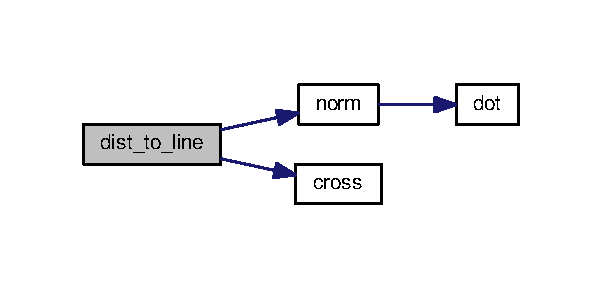
\includegraphics[width=289pt]{namespacesps_a55c6fe1c1fdf3c5a3e7b354dae205840_cgraph}
\end{center}
\end{figure}


\hypertarget{namespacesps_a00bcbe34e177c2a5ac0ec59f89998db2}{\index{sps@{sps}!dists\+\_\+most\+\_\+distant\+\_\+and\+\_\+closest@{dists\+\_\+most\+\_\+distant\+\_\+and\+\_\+closest}}
\index{dists\+\_\+most\+\_\+distant\+\_\+and\+\_\+closest@{dists\+\_\+most\+\_\+distant\+\_\+and\+\_\+closest}!sps@{sps}}
\subsubsection[{dists\+\_\+most\+\_\+distant\+\_\+and\+\_\+closest}]{\setlength{\rightskip}{0pt plus 5cm}void sps\+::dists\+\_\+most\+\_\+distant\+\_\+and\+\_\+closest (
\begin{DoxyParamCaption}
\item[{const sps\+::bbox\+\_\+t$<$ T $>$ \&}]{box0, }
\item[{const sps\+::bbox\+\_\+t$<$ T $>$ \&}]{box1, }
\item[{T $\ast$}]{dist\+Near, }
\item[{T $\ast$}]{dist\+Far}
\end{DoxyParamCaption}
)\hspace{0.3cm}{\ttfamily [inline]}}}\label{namespacesps_a00bcbe34e177c2a5ac0ec59f89998db2}


Here is the call graph for this function\+:\nopagebreak
\begin{figure}[H]
\begin{center}
\leavevmode
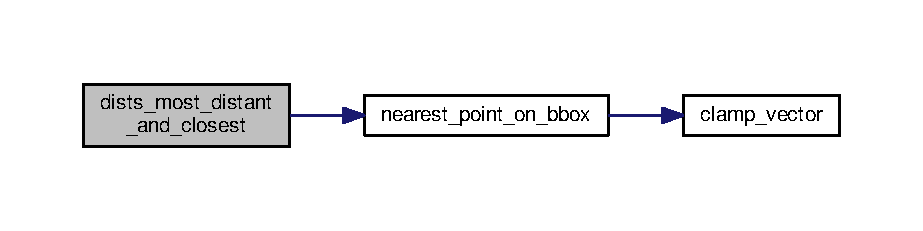
\includegraphics[width=350pt]{namespacesps_a00bcbe34e177c2a5ac0ec59f89998db2_cgraph}
\end{center}
\end{figure}


\hypertarget{namespacesps_a49b7bc999932466978a16485e1c6a98b}{\index{sps@{sps}!dot@{dot}}
\index{dot@{dot}!sps@{sps}}
\subsubsection[{dot}]{\setlength{\rightskip}{0pt plus 5cm}T sps\+::dot (
\begin{DoxyParamCaption}
\item[{const point\+\_\+t$<$ T $>$ \&}]{a, }
\item[{const point\+\_\+t$<$ T $>$ \&}]{b}
\end{DoxyParamCaption}
)\hspace{0.3cm}{\ttfamily [inline]}}}\label{namespacesps_a49b7bc999932466978a16485e1c6a98b}
Dot product of vectors or points


\begin{DoxyParams}{Parameters}
{\em a} & \\
\hline
{\em b} & \\
\hline
\end{DoxyParams}
\begin{DoxyReturn}{Returns}

\end{DoxyReturn}
\hypertarget{namespacesps_a5ba962916e1ba5c3114e45f153d80081}{\index{sps@{sps}!farthest\+\_\+point\+\_\+on\+\_\+bbox@{farthest\+\_\+point\+\_\+on\+\_\+bbox}}
\index{farthest\+\_\+point\+\_\+on\+\_\+bbox@{farthest\+\_\+point\+\_\+on\+\_\+bbox}!sps@{sps}}
\subsubsection[{farthest\+\_\+point\+\_\+on\+\_\+bbox}]{\setlength{\rightskip}{0pt plus 5cm}sps\+::point\+\_\+t$<$T$>$ sps\+::farthest\+\_\+point\+\_\+on\+\_\+bbox (
\begin{DoxyParamCaption}
\item[{const sps\+::point\+\_\+t$<$ T $>$ \&}]{point, }
\item[{const sps\+::bbox\+\_\+t$<$ T $>$ \&}]{box}
\end{DoxyParamCaption}
)\hspace{0.3cm}{\ttfamily [inline]}}}\label{namespacesps_a5ba962916e1ba5c3114e45f153d80081}
Farthest point on a box (from a point)


\begin{DoxyParams}{Parameters}
{\em point} & \\
\hline
{\em box} & \\
\hline
\end{DoxyParams}
\begin{DoxyReturn}{Returns}

\end{DoxyReturn}
\hypertarget{namespacesps_a49f2545f74f9a6cf30e04d428badaf27}{\index{sps@{sps}!nearest\+\_\+point\+\_\+on\+\_\+bbox@{nearest\+\_\+point\+\_\+on\+\_\+bbox}}
\index{nearest\+\_\+point\+\_\+on\+\_\+bbox@{nearest\+\_\+point\+\_\+on\+\_\+bbox}!sps@{sps}}
\subsubsection[{nearest\+\_\+point\+\_\+on\+\_\+bbox}]{\setlength{\rightskip}{0pt plus 5cm}sps\+::point\+\_\+t$<$T$>$ sps\+::nearest\+\_\+point\+\_\+on\+\_\+bbox (
\begin{DoxyParamCaption}
\item[{const sps\+::point\+\_\+t$<$ T $>$ \&}]{point, }
\item[{const sps\+::bbox\+\_\+t$<$ T $>$ \&}]{box}
\end{DoxyParamCaption}
)\hspace{0.3cm}{\ttfamily [inline]}}}\label{namespacesps_a49f2545f74f9a6cf30e04d428badaf27}
Nearest point on a box (from a point)


\begin{DoxyParams}{Parameters}
{\em point} & \\
\hline
{\em box} & \\
\hline
\end{DoxyParams}
\begin{DoxyReturn}{Returns}

\end{DoxyReturn}


Here is the call graph for this function\+:\nopagebreak
\begin{figure}[H]
\begin{center}
\leavevmode
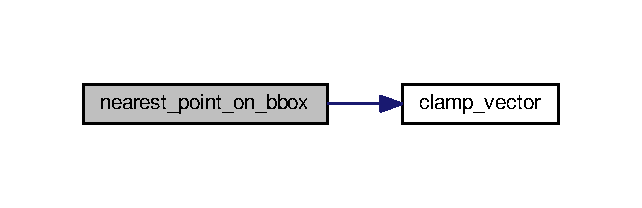
\includegraphics[width=308pt]{namespacesps_a49f2545f74f9a6cf30e04d428badaf27_cgraph}
\end{center}
\end{figure}


\hypertarget{namespacesps_ac8e58e03b1ed250e4dd83774401fb670}{\index{sps@{sps}!norm@{norm}}
\index{norm@{norm}!sps@{sps}}
\subsubsection[{norm}]{\setlength{\rightskip}{0pt plus 5cm}T sps\+::norm (
\begin{DoxyParamCaption}
\item[{const point\+\_\+t$<$ T $>$ \&}]{a}
\end{DoxyParamCaption}
)\hspace{0.3cm}{\ttfamily [inline]}}}\label{namespacesps_ac8e58e03b1ed250e4dd83774401fb670}
Norm of a vector or point


\begin{DoxyParams}{Parameters}
{\em a} & \\
\hline
\end{DoxyParams}
\begin{DoxyReturn}{Returns}
$\vert$a$\vert$ 
\end{DoxyReturn}


Here is the call graph for this function\+:\nopagebreak
\begin{figure}[H]
\begin{center}
\leavevmode
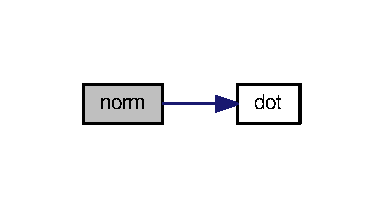
\includegraphics[width=184pt]{namespacesps_ac8e58e03b1ed250e4dd83774401fb670_cgraph}
\end{center}
\end{figure}


\hypertarget{namespacesps_a22175b6c56edce28e060aaddb0443215}{\index{sps@{sps}!operator$\ast$@{operator$\ast$}}
\index{operator$\ast$@{operator$\ast$}!sps@{sps}}
\subsubsection[{operator$\ast$}]{\setlength{\rightskip}{0pt plus 5cm}point\+\_\+t$<$T$>$ sps\+::operator$\ast$ (
\begin{DoxyParamCaption}
\item[{const T \&}]{a, }
\item[{const point\+\_\+t$<$ T $>$ \&}]{b}
\end{DoxyParamCaption}
)\hspace{0.3cm}{\ttfamily [inline]}}}\label{namespacesps_a22175b6c56edce28e060aaddb0443215}
Scalar multiplication of a vector or point


\begin{DoxyParams}{Parameters}
{\em a} & scalar \\
\hline
{\em b} & point\\
\hline
\end{DoxyParams}
\begin{DoxyReturn}{Returns}

\end{DoxyReturn}
\hypertarget{namespacesps_abcd3fabeb60a10d9ad05fc027c789e9e}{\index{sps@{sps}!operator+@{operator+}}
\index{operator+@{operator+}!sps@{sps}}
\subsubsection[{operator+}]{\setlength{\rightskip}{0pt plus 5cm}point\+\_\+t$<$T$>$ sps\+::operator+ (
\begin{DoxyParamCaption}
\item[{const point\+\_\+t$<$ T $>$ \&}]{a, }
\item[{const point\+\_\+t$<$ T $>$ \&}]{b}
\end{DoxyParamCaption}
)\hspace{0.3cm}{\ttfamily [inline]}}}\label{namespacesps_abcd3fabeb60a10d9ad05fc027c789e9e}
Add two points


\begin{DoxyParams}{Parameters}
{\em a} & \\
\hline
{\em b} & \\
\hline
\end{DoxyParams}
\begin{DoxyReturn}{Returns}
a + b 
\end{DoxyReturn}
\hypertarget{namespacesps_a634cb0a93cc6f57c45c79f7df04c8752}{\index{sps@{sps}!operator-\/@{operator-\/}}
\index{operator-\/@{operator-\/}!sps@{sps}}
\subsubsection[{operator-\/}]{\setlength{\rightskip}{0pt plus 5cm}point\+\_\+t$<$T$>$ sps\+::operator-\/ (
\begin{DoxyParamCaption}
\item[{const point\+\_\+t$<$ T $>$ \&}]{a, }
\item[{const point\+\_\+t$<$ T $>$ \&}]{b}
\end{DoxyParamCaption}
)\hspace{0.3cm}{\ttfamily [inline]}}}\label{namespacesps_a634cb0a93cc6f57c45c79f7df04c8752}
Subtract two points


\begin{DoxyParams}{Parameters}
{\em a} & \\
\hline
{\em b} & \\
\hline
\end{DoxyParams}
\begin{DoxyReturn}{Returns}
a -\/ b 
\end{DoxyReturn}
\hypertarget{namespacesps_a1f6bfb41fd1c17ffbe559cb6c9838487}{\index{sps@{sps}!operator$<$$<$@{operator$<$$<$}}
\index{operator$<$$<$@{operator$<$$<$}!sps@{sps}}
\subsubsection[{operator$<$$<$}]{\setlength{\rightskip}{0pt plus 5cm}std\+::ostream\& sps\+::operator$<$$<$ (
\begin{DoxyParamCaption}
\item[{std\+::ostream \&}]{out, }
\item[{const point\+\_\+t$<$ T $>$ \&}]{point}
\end{DoxyParamCaption}
)\hspace{0.3cm}{\ttfamily [inline]}}}\label{namespacesps_a1f6bfb41fd1c17ffbe559cb6c9838487}
Operator for printing points to a stream


\begin{DoxyParams}{Parameters}
{\em out} & \\
\hline
{\em point} & \\
\hline
\end{DoxyParams}
\begin{DoxyReturn}{Returns}

\end{DoxyReturn}
\hypertarget{namespacesps_a6d00662f3287276d877ae3e1e10b9c6e}{\index{sps@{sps}!sgn\+\_\+dist\+\_\+to\+\_\+plane@{sgn\+\_\+dist\+\_\+to\+\_\+plane}}
\index{sgn\+\_\+dist\+\_\+to\+\_\+plane@{sgn\+\_\+dist\+\_\+to\+\_\+plane}!sps@{sps}}
\subsubsection[{sgn\+\_\+dist\+\_\+to\+\_\+plane}]{\setlength{\rightskip}{0pt plus 5cm}T sps\+::sgn\+\_\+dist\+\_\+to\+\_\+plane (
\begin{DoxyParamCaption}
\item[{const point\+\_\+t$<$ T $>$ \&}]{point, }
\item[{const point\+\_\+t$<$ T $>$ \&}]{point\+On\+Plane, }
\item[{const point\+\_\+t$<$ T $>$ \&}]{unit\+Normal}
\end{DoxyParamCaption}
)\hspace{0.3cm}{\ttfamily [inline]}}}\label{namespacesps_a6d00662f3287276d877ae3e1e10b9c6e}
Signed distance from point to plane


\begin{DoxyParams}{Parameters}
{\em point} & \\
\hline
{\em point\+On\+Plane} & \\
\hline
{\em unit\+Normal} & \\
\hline
\end{DoxyParams}
\begin{DoxyReturn}{Returns}

\end{DoxyReturn}


Here is the call graph for this function\+:\nopagebreak
\begin{figure}[H]
\begin{center}
\leavevmode
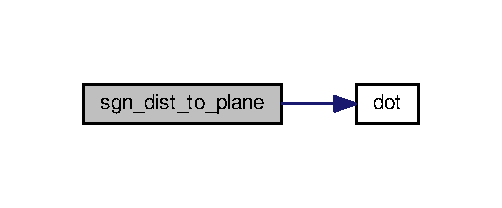
\includegraphics[width=241pt]{namespacesps_a6d00662f3287276d877ae3e1e10b9c6e_cgraph}
\end{center}
\end{figure}



\chapter{Class Documentation}
\hypertarget{classfnm_1_1Aperture}{\section{Aperture$<$ T $>$ Class Template Reference}
\label{classfnm_1_1Aperture}\index{Aperture$<$ T $>$@{Aperture$<$ T $>$}}
}


\hyperlink{classfnm_1_1Aperture}{Aperture} class.  




{\ttfamily \#include $<$fnm.\+hpp$>$}

\subsection*{Public Member Functions}
\begin{DoxyCompactItemize}
\item 
\hyperlink{classfnm_1_1Aperture_a3990298bb3b2d0cd9275a039d6bd8319}{Aperture} ()
\item 
\hyperlink{classfnm_1_1Aperture_a48761e9fd3f7270c9de20abce9a8bad5}{Aperture} (const size\+\_\+t n\+Elements, const T width, const T kerf, const T height)
\item 
\hyperlink{classfnm_1_1Aperture_acf8f763505318fa40717d41620560d3b}{$\sim$\+Aperture} ()
\item 
const size\+\_\+t \& \hyperlink{classfnm_1_1Aperture_ab0d91160f41e515aa56b4a961c528e32}{N\+Elements\+Get} () const 
\item 
const size\+\_\+t \& \hyperlink{classfnm_1_1Aperture_a5c28c71c5172cfe9ecce41f112297073}{N\+Sub\+Elements\+Get} () const 
\item 
void \hyperlink{classfnm_1_1Aperture_a63d391bb8c52d45c1ba48f765ce1943c}{Extent\+Get} (T $\ast$$\ast$coordinates, size\+\_\+t $\ast$n\+Dim, size\+\_\+t $\ast$n\+Limits) const 
\item 
T \hyperlink{classfnm_1_1Aperture_a5a2beeb4beb4cdac3ee643598eb43421}{Area\+Get} () const 
\item 
void \hyperlink{classfnm_1_1Aperture_a7f1c68283a50419ef55a3af3a2da7a18}{Phases\+Get} (T $\ast$$\ast$data, size\+\_\+t $\ast$n\+Data)
\item 
void \hyperlink{classfnm_1_1Aperture_a4af91355130ec0fe184a9ccd380b8ba1}{Delays\+Get} (T $\ast$$\ast$data, size\+\_\+t $\ast$n\+Data)
\item 
void \hyperlink{classfnm_1_1Aperture_a109e4080fa678b8ae57cfc4da2c9e364}{Rectangles\+Get} (T $\ast$$\ast$out, size\+\_\+t $\ast$n\+Elements, size\+\_\+t $\ast$n\+Sub\+Elements, size\+\_\+t $\ast$n\+Params) const 
\item 
void \hyperlink{classfnm_1_1Aperture_ad5917a3f2f62df8cf44a9a8db7fd6fde}{Positions\+Get} (T $\ast$$\ast$out, size\+\_\+t $\ast$n\+Elements, size\+\_\+t $\ast$n\+Params) const 
\item 
void \hyperlink{classfnm_1_1Aperture_ab10c2efc99c80b25caa3abab50b14856}{Positions\+Set} (const T $\ast$pos, const size\+\_\+t n\+Positions, const size\+\_\+t n\+Dim)
\item 
void \hyperlink{classfnm_1_1Aperture_aed74195d0a3d7bb7bf42a9d97691ebbf}{Focus\+Get} (T o\+Focus\mbox{[}3\mbox{]}) const 
\item 
void \hyperlink{classfnm_1_1Aperture_aa2a0b49036000182665d4218489bf2e4}{Focus\+Set} (const T i\+Focus\mbox{[}3\mbox{]})
\item 
int \hyperlink{classfnm_1_1Aperture_a77d8cd829340ff37dfdd502b1b47f5fe}{Focusing\+Type\+Get} () const 
\item 
void \hyperlink{classfnm_1_1Aperture_a7ec287084c79fb733e2ff5a471387f5f}{Focusing\+Type\+Set} (const int i\+Focusing\+Type)
\item 
const size\+\_\+t \& \hyperlink{classfnm_1_1Aperture_a6697d507490040a87dbd4a3d67a13fc7}{N\+Threads\+Get} () const 
\item 
void \hyperlink{classfnm_1_1Aperture_a4cfa8bc49387e8ab7d2ac23ed1b1ccf6}{N\+Threads\+Set} (const size\+\_\+t \&n\+Threads)
\item 
const T \& \hyperlink{classfnm_1_1Aperture_afd19e2ba296df82e56e58ebd151c7a71}{F0\+Get} () const 
\item 
void \hyperlink{classfnm_1_1Aperture_a67f51a08d98cc368cc4c4a6414edb3fa}{F0\+Set} (const T f0)
\item 
void \hyperlink{classfnm_1_1Aperture_adffaa1f7cab073f40c532fc58cf6e55c}{Sys\+Parm\+Set} (const \hyperlink{structfnm_1_1sysparm__t}{sysparm\+\_\+t}$<$ T $>$ $\ast$arg)
\item 
const T \& \hyperlink{classfnm_1_1Aperture_a315ccdf731ff56729bfa8f5a1305a345}{C\+Get} () const 
\item 
void \hyperlink{classfnm_1_1Aperture_a49d9268feca025de3dc648abf6a8b3e1}{C\+Set} (const T c)
\item 
void \hyperlink{classfnm_1_1Aperture_a8bab384e28c3bb00f9e0a521c30ef64c}{Elements\+Get} (T $\ast$$\ast$out, size\+\_\+t $\ast$n\+Elements, size\+\_\+t $\ast$n\+Params) const 
\item 
bool \hyperlink{classfnm_1_1Aperture_a907987dd1686d882fdd35fd677d9c56d}{Elements\+Set} (const T $\ast$pos, const size\+\_\+t n\+Positions, const size\+\_\+t n\+Dim)  throw (std\+::runtime\+\_\+error)
\begin{DoxyCompactList}\small\item\em Set element positions. \end{DoxyCompactList}\item 
void \hyperlink{classfnm_1_1Aperture_abaa41240b00a74b090b718872a44fac8}{Sub\+Elements\+Get} (T $\ast$$\ast$out, size\+\_\+t $\ast$n\+Elements, size\+\_\+t $\ast$n\+Sub\+Elements, size\+\_\+t $\ast$n\+Params) const 
\item 
bool \hyperlink{classfnm_1_1Aperture_abeee1842f9d811720380ee3ba3f059f5}{Sub\+Elements\+Set} (const T $\ast$pos, const size\+\_\+t n\+Elements, const size\+\_\+t n\+Sub\+Elements\+Per\+Element, const size\+\_\+t n\+Dim)
\item 
const size\+\_\+t \& \hyperlink{classfnm_1_1Aperture_a67496fa5642e3becc2531aa0bee54041}{N\+Div\+W\+Get} () const 
\item 
void \hyperlink{classfnm_1_1Aperture_a85ddb5a2c36e41d4b2b4714372abe931}{N\+Div\+W\+Set} (const size\+\_\+t n\+Div\+W)
\item 
const size\+\_\+t \& \hyperlink{classfnm_1_1Aperture_a60d4b397ce55604848f2b8b92ce23f51}{N\+Div\+H\+Get} () const 
\item 
void \hyperlink{classfnm_1_1Aperture_aa01cd8acfe2f084f20172afb68c2983a}{N\+Div\+H\+Set} (const size\+\_\+t n\+Div\+H)
\item 
void \hyperlink{classfnm_1_1Aperture_a289829b660a5ef3e4cdf4bbbae5d9dbf}{Apodization\+Get} (T $\ast$$\ast$data, size\+\_\+t $\ast$n\+Data) const 
\item 
void \hyperlink{classfnm_1_1Aperture_a6ec932bbf0a8cc4d51df50f54f9dced0}{Apodization\+Set} (const T $\ast$data, const size\+\_\+t n\+Data)
\item 
void \hyperlink{classfnm_1_1Aperture_af409f86faed17c9b7f2cf098ec4ba9e8}{Progress\+Bar\+Set} (sps\+::\+Progress\+Bar\+Interface $\ast$pbar)
\item 
void \hyperlink{classfnm_1_1Aperture_a9508a8d8cebc92f46019929e14f288b3}{Focus\+Update} ()
\item 
int \hyperlink{classfnm_1_1Aperture_a10975da23ed3050191c892cd54b7e3f3}{Calc\+Asa} (const T $\ast$y0, const size\+\_\+t nx, const size\+\_\+t ny, const T dx, const T dy, const size\+\_\+t Nx, const size\+\_\+t Ny, std\+::complex$<$ T $>$ $\ast$$\ast$p1, size\+\_\+t $\ast$onx, size\+\_\+t $\ast$ony, size\+\_\+t $\ast$onz)
\end{DoxyCompactItemize}
{\bf }\par
\begin{DoxyCompactItemize}
\item 
int \hyperlink{classfnm_1_1Aperture_aa12e26aae03e1310de3b419d6eda061c}{Calc\+Cw\+Field\+Ref} (const T $\ast$pos, const size\+\_\+t n\+Positions, const size\+\_\+t n\+Dim, std\+::complex$<$ T $>$ $\ast$$\ast$odata, size\+\_\+t $\ast$n\+Out\+Positions)
\item 
int \hyperlink{classfnm_1_1Aperture_affc58ecd7f649cbeab23b676f308f185}{Calc\+Cw\+Fast} (const T $\ast$pos, const size\+\_\+t n\+Positions, const size\+\_\+t n\+Dim, std\+::complex$<$ T $>$ $\ast$$\ast$odata, size\+\_\+t $\ast$n\+Out\+Positions)
\item 
int \hyperlink{classfnm_1_1Aperture_ac02ec8b45ead743c15fd64127a9cff67}{Calc\+Cw\+Field} (const T $\ast$pos, const size\+\_\+t n\+Positions, const size\+\_\+t n\+Dim, std\+::complex$<$ T $>$ $\ast$$\ast$odata, size\+\_\+t $\ast$n\+Out\+Positions)
\item 
int \hyperlink{classfnm_1_1Aperture_a00d23fa1c2a6c6547606702a72d71aa1}{Calc\+Cw\+Field2} (const T $\ast$pos, const size\+\_\+t n\+Positions, const size\+\_\+t n\+Dim, std\+::complex$<$ T $>$ $\ast$$\ast$odata, size\+\_\+t $\ast$n\+Out\+Positions)
\end{DoxyCompactItemize}

\subsection*{Static Public Attributes}
\begin{DoxyCompactItemize}
\item 
static const size\+\_\+t \hyperlink{classfnm_1_1Aperture_ac08006cf2e1c77856e2332b6d98ca861}{n\+Vertices\+Per\+Element} = 4
\item 
static const size\+\_\+t \hyperlink{classfnm_1_1Aperture_adaffd7c31c339cecbb613daa7eae4f64}{n\+Element\+Pos\+Parameters} = 8
\item 
static \hyperlink{structfnm_1_1sysparm__t}{sysparm\+\_\+t}$<$ T $>$ \hyperlink{classfnm_1_1Aperture_a7f24436369eec62f8d62cd18fc1eda03}{\+\_\+sysparm}
\begin{DoxyCompactList}\small\item\em System parameters (We could make a long list of functions friends of \hyperlink{classfnm_1_1Aperture}{Aperture}) \end{DoxyCompactList}\item 
static T \hyperlink{classfnm_1_1Aperture_aeba68ad214d4eb5ef51b3f3763d099dd}{fs}
\end{DoxyCompactItemize}


\subsection{Detailed Description}
\subsubsection*{template$<$class T$>$class fnm\+::\+Aperture$<$ T $>$}

\hyperlink{classfnm_1_1Aperture}{Aperture} class. 

A class representing an aperture 

\subsection{Constructor \& Destructor Documentation}
\hypertarget{classfnm_1_1Aperture_a3990298bb3b2d0cd9275a039d6bd8319}{\index{fnm\+::\+Aperture@{fnm\+::\+Aperture}!Aperture@{Aperture}}
\index{Aperture@{Aperture}!fnm\+::\+Aperture@{fnm\+::\+Aperture}}
\subsubsection[{Aperture}]{\setlength{\rightskip}{0pt plus 5cm}{\bf Aperture} (
\begin{DoxyParamCaption}
{}
\end{DoxyParamCaption}
)}}\label{classfnm_1_1Aperture_a3990298bb3b2d0cd9275a039d6bd8319}
Constructor \hypertarget{classfnm_1_1Aperture_a48761e9fd3f7270c9de20abce9a8bad5}{\index{fnm\+::\+Aperture@{fnm\+::\+Aperture}!Aperture@{Aperture}}
\index{Aperture@{Aperture}!fnm\+::\+Aperture@{fnm\+::\+Aperture}}
\subsubsection[{Aperture}]{\setlength{\rightskip}{0pt plus 5cm}{\bf Aperture} (
\begin{DoxyParamCaption}
\item[{const size\+\_\+t}]{n\+Elements, }
\item[{const T}]{width, }
\item[{const T}]{kerf, }
\item[{const T}]{height}
\end{DoxyParamCaption}
)}}\label{classfnm_1_1Aperture_a48761e9fd3f7270c9de20abce9a8bad5}
Constructor for linear array


\begin{DoxyParams}{Parameters}
{\em n\+Elements} & \\
\hline
{\em width} & \\
\hline
{\em kerf} & \\
\hline
{\em height} & \\
\hline
\end{DoxyParams}
\begin{DoxyReturn}{Returns}

\end{DoxyReturn}
\hypertarget{classfnm_1_1Aperture_acf8f763505318fa40717d41620560d3b}{\index{fnm\+::\+Aperture@{fnm\+::\+Aperture}!````~Aperture@{$\sim$\+Aperture}}
\index{````~Aperture@{$\sim$\+Aperture}!fnm\+::\+Aperture@{fnm\+::\+Aperture}}
\subsubsection[{$\sim$\+Aperture}]{\setlength{\rightskip}{0pt plus 5cm}$\sim${\bf Aperture} (
\begin{DoxyParamCaption}
{}
\end{DoxyParamCaption}
)}}\label{classfnm_1_1Aperture_acf8f763505318fa40717d41620560d3b}
Destructor

\begin{DoxyReturn}{Returns}

\end{DoxyReturn}


\subsection{Member Function Documentation}
\hypertarget{classfnm_1_1Aperture_a289829b660a5ef3e4cdf4bbbae5d9dbf}{\index{fnm\+::\+Aperture@{fnm\+::\+Aperture}!Apodization\+Get@{Apodization\+Get}}
\index{Apodization\+Get@{Apodization\+Get}!fnm\+::\+Aperture@{fnm\+::\+Aperture}}
\subsubsection[{Apodization\+Get}]{\setlength{\rightskip}{0pt plus 5cm}void Apodization\+Get (
\begin{DoxyParamCaption}
\item[{T $\ast$$\ast$}]{data, }
\item[{size\+\_\+t $\ast$}]{n\+Data}
\end{DoxyParamCaption}
) const}}\label{classfnm_1_1Aperture_a289829b660a5ef3e4cdf4bbbae5d9dbf}
Get apodization


\begin{DoxyParams}{Parameters}
{\em data} & \\
\hline
{\em n\+Data} & \\
\hline
\end{DoxyParams}
\hypertarget{classfnm_1_1Aperture_a6ec932bbf0a8cc4d51df50f54f9dced0}{\index{fnm\+::\+Aperture@{fnm\+::\+Aperture}!Apodization\+Set@{Apodization\+Set}}
\index{Apodization\+Set@{Apodization\+Set}!fnm\+::\+Aperture@{fnm\+::\+Aperture}}
\subsubsection[{Apodization\+Set}]{\setlength{\rightskip}{0pt plus 5cm}void Apodization\+Set (
\begin{DoxyParamCaption}
\item[{const T $\ast$}]{data, }
\item[{const size\+\_\+t}]{n\+Data}
\end{DoxyParamCaption}
)}}\label{classfnm_1_1Aperture_a6ec932bbf0a8cc4d51df50f54f9dced0}
Set apodization


\begin{DoxyParams}{Parameters}
{\em data} & \\
\hline
{\em n\+Data} & \\
\hline
\end{DoxyParams}
\hypertarget{classfnm_1_1Aperture_a5a2beeb4beb4cdac3ee643598eb43421}{\index{fnm\+::\+Aperture@{fnm\+::\+Aperture}!Area\+Get@{Area\+Get}}
\index{Area\+Get@{Area\+Get}!fnm\+::\+Aperture@{fnm\+::\+Aperture}}
\subsubsection[{Area\+Get}]{\setlength{\rightskip}{0pt plus 5cm}T Area\+Get (
\begin{DoxyParamCaption}
{}
\end{DoxyParamCaption}
) const}}\label{classfnm_1_1Aperture_a5a2beeb4beb4cdac3ee643598eb43421}
\hypertarget{classfnm_1_1Aperture_a10975da23ed3050191c892cd54b7e3f3}{\index{fnm\+::\+Aperture@{fnm\+::\+Aperture}!Calc\+Asa@{Calc\+Asa}}
\index{Calc\+Asa@{Calc\+Asa}!fnm\+::\+Aperture@{fnm\+::\+Aperture}}
\subsubsection[{Calc\+Asa}]{\setlength{\rightskip}{0pt plus 5cm}int Calc\+Asa (
\begin{DoxyParamCaption}
\item[{const T $\ast$}]{y0, }
\item[{const size\+\_\+t}]{nx, }
\item[{const size\+\_\+t}]{ny, }
\item[{const T}]{dx, }
\item[{const T}]{dy, }
\item[{const size\+\_\+t}]{Nx, }
\item[{const size\+\_\+t}]{Ny, }
\item[{std\+::complex$<$ T $>$ $\ast$$\ast$}]{p1, }
\item[{size\+\_\+t $\ast$}]{onx, }
\item[{size\+\_\+t $\ast$}]{ony, }
\item[{size\+\_\+t $\ast$}]{onz}
\end{DoxyParamCaption}
)}}\label{classfnm_1_1Aperture_a10975da23ed3050191c892cd54b7e3f3}
Experimental functions \hypertarget{classfnm_1_1Aperture_affc58ecd7f649cbeab23b676f308f185}{\index{fnm\+::\+Aperture@{fnm\+::\+Aperture}!Calc\+Cw\+Fast@{Calc\+Cw\+Fast}}
\index{Calc\+Cw\+Fast@{Calc\+Cw\+Fast}!fnm\+::\+Aperture@{fnm\+::\+Aperture}}
\subsubsection[{Calc\+Cw\+Fast}]{\setlength{\rightskip}{0pt plus 5cm}int Calc\+Cw\+Fast (
\begin{DoxyParamCaption}
\item[{const T $\ast$}]{pos, }
\item[{const size\+\_\+t}]{n\+Positions, }
\item[{const size\+\_\+t}]{n\+Dim, }
\item[{std\+::complex$<$ T $>$ $\ast$$\ast$}]{odata, }
\item[{size\+\_\+t $\ast$}]{n\+Out\+Positions}
\end{DoxyParamCaption}
)}}\label{classfnm_1_1Aperture_affc58ecd7f649cbeab23b676f308f185}
Compute C\+W response at multiple positions (uses S\+I\+M\+D). The ranges of integration are reduced to give the most accurate result with less abcissas.


\begin{DoxyParams}{Parameters}
{\em pos} & \\
\hline
{\em n\+Positions} & \\
\hline
{\em n\+Dim} & \\
\hline
{\em odata} & \\
\hline
{\em n\+Out\+Positions} & \\
\hline
\end{DoxyParams}
\hypertarget{classfnm_1_1Aperture_ac02ec8b45ead743c15fd64127a9cff67}{\index{fnm\+::\+Aperture@{fnm\+::\+Aperture}!Calc\+Cw\+Field@{Calc\+Cw\+Field}}
\index{Calc\+Cw\+Field@{Calc\+Cw\+Field}!fnm\+::\+Aperture@{fnm\+::\+Aperture}}
\subsubsection[{Calc\+Cw\+Field}]{\setlength{\rightskip}{0pt plus 5cm}int Calc\+Cw\+Field (
\begin{DoxyParamCaption}
\item[{const T $\ast$}]{pos, }
\item[{const size\+\_\+t}]{n\+Positions, }
\item[{const size\+\_\+t}]{n\+Dim, }
\item[{std\+::complex$<$ T $>$ $\ast$$\ast$}]{odata, }
\item[{size\+\_\+t $\ast$}]{n\+Out\+Positions}
\end{DoxyParamCaption}
)}}\label{classfnm_1_1Aperture_ac02ec8b45ead743c15fd64127a9cff67}
Compute C\+W response at multiple positions. The range of integration is naive so it is accurate when projections lie inside an element, but requires a huge amount of abcissas to get a usuable result, when projections lie outside an element.

T\+O\+D\+O\+: Remove when Calc\+Cw\+Field\+Ref is fixed


\begin{DoxyParams}{Parameters}
{\em pos} & \\
\hline
{\em n\+Positions} & \\
\hline
{\em n\+Dim} & \\
\hline
{\em odata} & \\
\hline
{\em n\+Out\+Positions} & \\
\hline
\end{DoxyParams}
\hypertarget{classfnm_1_1Aperture_a00d23fa1c2a6c6547606702a72d71aa1}{\index{fnm\+::\+Aperture@{fnm\+::\+Aperture}!Calc\+Cw\+Field2@{Calc\+Cw\+Field2}}
\index{Calc\+Cw\+Field2@{Calc\+Cw\+Field2}!fnm\+::\+Aperture@{fnm\+::\+Aperture}}
\subsubsection[{Calc\+Cw\+Field2}]{\setlength{\rightskip}{0pt plus 5cm}int Calc\+Cw\+Field2 (
\begin{DoxyParamCaption}
\item[{const T $\ast$}]{pos, }
\item[{const size\+\_\+t}]{n\+Positions, }
\item[{const size\+\_\+t}]{n\+Dim, }
\item[{std\+::complex$<$ T $>$ $\ast$$\ast$}]{odata, }
\item[{size\+\_\+t $\ast$}]{n\+Out\+Positions}
\end{DoxyParamCaption}
)}}\label{classfnm_1_1Aperture_a00d23fa1c2a6c6547606702a72d71aa1}
Same as Calc\+Cw\+Field, but uses S\+I\+M\+D.

T\+O\+D\+O\+: Remove when Calc\+Cw\+Field\+Ref is fixed


\begin{DoxyParams}{Parameters}
{\em pos} & \\
\hline
{\em n\+Positions} & \\
\hline
{\em n\+Dim} & \\
\hline
{\em odata} & \\
\hline
{\em n\+Out\+Positions} & \\
\hline
\end{DoxyParams}
\begin{DoxyReturn}{Returns}

\end{DoxyReturn}
\hypertarget{classfnm_1_1Aperture_aa12e26aae03e1310de3b419d6eda061c}{\index{fnm\+::\+Aperture@{fnm\+::\+Aperture}!Calc\+Cw\+Field\+Ref@{Calc\+Cw\+Field\+Ref}}
\index{Calc\+Cw\+Field\+Ref@{Calc\+Cw\+Field\+Ref}!fnm\+::\+Aperture@{fnm\+::\+Aperture}}
\subsubsection[{Calc\+Cw\+Field\+Ref}]{\setlength{\rightskip}{0pt plus 5cm}int Calc\+Cw\+Field\+Ref (
\begin{DoxyParamCaption}
\item[{const T $\ast$}]{pos, }
\item[{const size\+\_\+t}]{n\+Positions, }
\item[{const size\+\_\+t}]{n\+Dim, }
\item[{std\+::complex$<$ T $>$ $\ast$$\ast$}]{odata, }
\item[{size\+\_\+t $\ast$}]{n\+Out\+Positions}
\end{DoxyParamCaption}
)}}\label{classfnm_1_1Aperture_aa12e26aae03e1310de3b419d6eda061c}
Compute C\+W response at multiple positions. Reference implementation. The ranges of integration are reduced to give the most accurate result with less abcissas.


\begin{DoxyParams}{Parameters}
{\em pos} & \\
\hline
{\em n\+Positions} & \\
\hline
{\em n\+Dim} & \\
\hline
{\em odata} & \\
\hline
{\em n\+Out\+Positions} & \\
\hline
\end{DoxyParams}
\hypertarget{classfnm_1_1Aperture_a315ccdf731ff56729bfa8f5a1305a345}{\index{fnm\+::\+Aperture@{fnm\+::\+Aperture}!C\+Get@{C\+Get}}
\index{C\+Get@{C\+Get}!fnm\+::\+Aperture@{fnm\+::\+Aperture}}
\subsubsection[{C\+Get}]{\setlength{\rightskip}{0pt plus 5cm}const T\& C\+Get (
\begin{DoxyParamCaption}
{}
\end{DoxyParamCaption}
) const}}\label{classfnm_1_1Aperture_a315ccdf731ff56729bfa8f5a1305a345}
Get speed of sound

\begin{DoxyReturn}{Returns}

\end{DoxyReturn}
\hypertarget{classfnm_1_1Aperture_a49d9268feca025de3dc648abf6a8b3e1}{\index{fnm\+::\+Aperture@{fnm\+::\+Aperture}!C\+Set@{C\+Set}}
\index{C\+Set@{C\+Set}!fnm\+::\+Aperture@{fnm\+::\+Aperture}}
\subsubsection[{C\+Set}]{\setlength{\rightskip}{0pt plus 5cm}void C\+Set (
\begin{DoxyParamCaption}
\item[{const T}]{c}
\end{DoxyParamCaption}
)}}\label{classfnm_1_1Aperture_a49d9268feca025de3dc648abf6a8b3e1}
Set speed of sound


\begin{DoxyParams}{Parameters}
{\em c} & \\
\hline
\end{DoxyParams}
\hypertarget{classfnm_1_1Aperture_a4af91355130ec0fe184a9ccd380b8ba1}{\index{fnm\+::\+Aperture@{fnm\+::\+Aperture}!Delays\+Get@{Delays\+Get}}
\index{Delays\+Get@{Delays\+Get}!fnm\+::\+Aperture@{fnm\+::\+Aperture}}
\subsubsection[{Delays\+Get}]{\setlength{\rightskip}{0pt plus 5cm}void Delays\+Get (
\begin{DoxyParamCaption}
\item[{T $\ast$$\ast$}]{data, }
\item[{size\+\_\+t $\ast$}]{n\+Data}
\end{DoxyParamCaption}
)}}\label{classfnm_1_1Aperture_a4af91355130ec0fe184a9ccd380b8ba1}
Get delays of elements


\begin{DoxyParams}{Parameters}
{\em data} & \\
\hline
{\em n\+Data} & \\
\hline
\end{DoxyParams}
\hypertarget{classfnm_1_1Aperture_a8bab384e28c3bb00f9e0a521c30ef64c}{\index{fnm\+::\+Aperture@{fnm\+::\+Aperture}!Elements\+Get@{Elements\+Get}}
\index{Elements\+Get@{Elements\+Get}!fnm\+::\+Aperture@{fnm\+::\+Aperture}}
\subsubsection[{Elements\+Get}]{\setlength{\rightskip}{0pt plus 5cm}void Elements\+Get (
\begin{DoxyParamCaption}
\item[{T $\ast$$\ast$}]{out, }
\item[{size\+\_\+t $\ast$}]{n\+Elements, }
\item[{size\+\_\+t $\ast$}]{n\+Params}
\end{DoxyParamCaption}
) const}}\label{classfnm_1_1Aperture_a8bab384e28c3bb00f9e0a521c30ef64c}
Get element definitions


\begin{DoxyParams}{Parameters}
{\em out} & \\
\hline
{\em n\+Elements} & \\
\hline
{\em n\+Params} & \\
\hline
\end{DoxyParams}
\hypertarget{classfnm_1_1Aperture_a907987dd1686d882fdd35fd677d9c56d}{\index{fnm\+::\+Aperture@{fnm\+::\+Aperture}!Elements\+Set@{Elements\+Set}}
\index{Elements\+Set@{Elements\+Set}!fnm\+::\+Aperture@{fnm\+::\+Aperture}}
\subsubsection[{Elements\+Set}]{\setlength{\rightskip}{0pt plus 5cm}bool Elements\+Set (
\begin{DoxyParamCaption}
\item[{const T $\ast$}]{pos, }
\item[{const size\+\_\+t}]{n\+Positions, }
\item[{const size\+\_\+t}]{n\+Dim}
\end{DoxyParamCaption}
) throw  std\+::runtime\+\_\+error) }}\label{classfnm_1_1Aperture_a907987dd1686d882fdd35fd677d9c56d}


Set element positions. 


\begin{DoxyParams}{Parameters}
{\em pos} & Input data T\mbox{[}n\+Elements\mbox{]}\mbox{[}8\mbox{]} \\
\hline
{\em n\+Positions} & \\
\hline
{\em n\+Dim} & Must equal 8 \\
\hline
\end{DoxyParams}

\begin{DoxyExceptions}{Exceptions}
{\em std\+::runtime\+\_\+error} & n\+Dim != 8 \\
\hline
\end{DoxyExceptions}
\begin{DoxyReturn}{Returns}
true on success 
\end{DoxyReturn}
\hypertarget{classfnm_1_1Aperture_a63d391bb8c52d45c1ba48f765ce1943c}{\index{fnm\+::\+Aperture@{fnm\+::\+Aperture}!Extent\+Get@{Extent\+Get}}
\index{Extent\+Get@{Extent\+Get}!fnm\+::\+Aperture@{fnm\+::\+Aperture}}
\subsubsection[{Extent\+Get}]{\setlength{\rightskip}{0pt plus 5cm}void Extent\+Get (
\begin{DoxyParamCaption}
\item[{T $\ast$$\ast$}]{coordinates, }
\item[{size\+\_\+t $\ast$}]{n\+Dim, }
\item[{size\+\_\+t $\ast$}]{n\+Limits}
\end{DoxyParamCaption}
) const}}\label{classfnm_1_1Aperture_a63d391bb8c52d45c1ba48f765ce1943c}
\hypertarget{classfnm_1_1Aperture_afd19e2ba296df82e56e58ebd151c7a71}{\index{fnm\+::\+Aperture@{fnm\+::\+Aperture}!F0\+Get@{F0\+Get}}
\index{F0\+Get@{F0\+Get}!fnm\+::\+Aperture@{fnm\+::\+Aperture}}
\subsubsection[{F0\+Get}]{\setlength{\rightskip}{0pt plus 5cm}const T\& F0\+Get (
\begin{DoxyParamCaption}
{}
\end{DoxyParamCaption}
) const}}\label{classfnm_1_1Aperture_afd19e2ba296df82e56e58ebd151c7a71}
Get center frequency

\begin{DoxyReturn}{Returns}

\end{DoxyReturn}
\hypertarget{classfnm_1_1Aperture_a67f51a08d98cc368cc4c4a6414edb3fa}{\index{fnm\+::\+Aperture@{fnm\+::\+Aperture}!F0\+Set@{F0\+Set}}
\index{F0\+Set@{F0\+Set}!fnm\+::\+Aperture@{fnm\+::\+Aperture}}
\subsubsection[{F0\+Set}]{\setlength{\rightskip}{0pt plus 5cm}void F0\+Set (
\begin{DoxyParamCaption}
\item[{const T}]{f0}
\end{DoxyParamCaption}
)}}\label{classfnm_1_1Aperture_a67f51a08d98cc368cc4c4a6414edb3fa}
Set center frequency


\begin{DoxyParams}{Parameters}
{\em f0} & \\
\hline
\end{DoxyParams}
\hypertarget{classfnm_1_1Aperture_aed74195d0a3d7bb7bf42a9d97691ebbf}{\index{fnm\+::\+Aperture@{fnm\+::\+Aperture}!Focus\+Get@{Focus\+Get}}
\index{Focus\+Get@{Focus\+Get}!fnm\+::\+Aperture@{fnm\+::\+Aperture}}
\subsubsection[{Focus\+Get}]{\setlength{\rightskip}{0pt plus 5cm}void Focus\+Get (
\begin{DoxyParamCaption}
\item[{T}]{o\+Focus\mbox{[}3\mbox{]}}
\end{DoxyParamCaption}
) const}}\label{classfnm_1_1Aperture_aed74195d0a3d7bb7bf42a9d97691ebbf}
Get focus point or virtual source


\begin{DoxyParams}{Parameters}
{\em o\+Focus} & \\
\hline
\end{DoxyParams}
\hypertarget{classfnm_1_1Aperture_a77d8cd829340ff37dfdd502b1b47f5fe}{\index{fnm\+::\+Aperture@{fnm\+::\+Aperture}!Focusing\+Type\+Get@{Focusing\+Type\+Get}}
\index{Focusing\+Type\+Get@{Focusing\+Type\+Get}!fnm\+::\+Aperture@{fnm\+::\+Aperture}}
\subsubsection[{Focusing\+Type\+Get}]{\setlength{\rightskip}{0pt plus 5cm}int Focusing\+Type\+Get (
\begin{DoxyParamCaption}
{}
\end{DoxyParamCaption}
) const}}\label{classfnm_1_1Aperture_a77d8cd829340ff37dfdd502b1b47f5fe}
Get focus type used


\begin{DoxyParams}{Parameters}
{\em o\+Focus} & \\
\hline
\end{DoxyParams}
\hypertarget{classfnm_1_1Aperture_a7ec287084c79fb733e2ff5a471387f5f}{\index{fnm\+::\+Aperture@{fnm\+::\+Aperture}!Focusing\+Type\+Set@{Focusing\+Type\+Set}}
\index{Focusing\+Type\+Set@{Focusing\+Type\+Set}!fnm\+::\+Aperture@{fnm\+::\+Aperture}}
\subsubsection[{Focusing\+Type\+Set}]{\setlength{\rightskip}{0pt plus 5cm}void Focusing\+Type\+Set (
\begin{DoxyParamCaption}
\item[{const int}]{i\+Focusing\+Type}
\end{DoxyParamCaption}
)}}\label{classfnm_1_1Aperture_a7ec287084c79fb733e2ff5a471387f5f}
Set focus type used


\begin{DoxyParams}{Parameters}
{\em i\+Focus} & \\
\hline
\end{DoxyParams}
\hypertarget{classfnm_1_1Aperture_aa2a0b49036000182665d4218489bf2e4}{\index{fnm\+::\+Aperture@{fnm\+::\+Aperture}!Focus\+Set@{Focus\+Set}}
\index{Focus\+Set@{Focus\+Set}!fnm\+::\+Aperture@{fnm\+::\+Aperture}}
\subsubsection[{Focus\+Set}]{\setlength{\rightskip}{0pt plus 5cm}void Focus\+Set (
\begin{DoxyParamCaption}
\item[{const T}]{i\+Focus\mbox{[}3\mbox{]}}
\end{DoxyParamCaption}
)}}\label{classfnm_1_1Aperture_aa2a0b49036000182665d4218489bf2e4}
Set focus point or virtual source


\begin{DoxyParams}{Parameters}
{\em i\+Focus} & \\
\hline
\end{DoxyParams}
\hypertarget{classfnm_1_1Aperture_a9508a8d8cebc92f46019929e14f288b3}{\index{fnm\+::\+Aperture@{fnm\+::\+Aperture}!Focus\+Update@{Focus\+Update}}
\index{Focus\+Update@{Focus\+Update}!fnm\+::\+Aperture@{fnm\+::\+Aperture}}
\subsubsection[{Focus\+Update}]{\setlength{\rightskip}{0pt plus 5cm}void Focus\+Update (
\begin{DoxyParamCaption}
{}
\end{DoxyParamCaption}
)}}\label{classfnm_1_1Aperture_a9508a8d8cebc92f46019929e14f288b3}
Update phases after setting focus. This function is used by all methods for adjusting phases for focusing. \hypertarget{classfnm_1_1Aperture_a60d4b397ce55604848f2b8b92ce23f51}{\index{fnm\+::\+Aperture@{fnm\+::\+Aperture}!N\+Div\+H\+Get@{N\+Div\+H\+Get}}
\index{N\+Div\+H\+Get@{N\+Div\+H\+Get}!fnm\+::\+Aperture@{fnm\+::\+Aperture}}
\subsubsection[{N\+Div\+H\+Get}]{\setlength{\rightskip}{0pt plus 5cm}const size\+\_\+t\& N\+Div\+H\+Get (
\begin{DoxyParamCaption}
{}
\end{DoxyParamCaption}
) const}}\label{classfnm_1_1Aperture_a60d4b397ce55604848f2b8b92ce23f51}
Get number of height abcissas

\begin{DoxyReturn}{Returns}

\end{DoxyReturn}
\hypertarget{classfnm_1_1Aperture_aa01cd8acfe2f084f20172afb68c2983a}{\index{fnm\+::\+Aperture@{fnm\+::\+Aperture}!N\+Div\+H\+Set@{N\+Div\+H\+Set}}
\index{N\+Div\+H\+Set@{N\+Div\+H\+Set}!fnm\+::\+Aperture@{fnm\+::\+Aperture}}
\subsubsection[{N\+Div\+H\+Set}]{\setlength{\rightskip}{0pt plus 5cm}void N\+Div\+H\+Set (
\begin{DoxyParamCaption}
\item[{const size\+\_\+t}]{n\+Div\+H}
\end{DoxyParamCaption}
)}}\label{classfnm_1_1Aperture_aa01cd8acfe2f084f20172afb68c2983a}
Set number of height abicissas


\begin{DoxyParams}{Parameters}
{\em n\+Div\+H} & \\
\hline
\end{DoxyParams}
\hypertarget{classfnm_1_1Aperture_a67496fa5642e3becc2531aa0bee54041}{\index{fnm\+::\+Aperture@{fnm\+::\+Aperture}!N\+Div\+W\+Get@{N\+Div\+W\+Get}}
\index{N\+Div\+W\+Get@{N\+Div\+W\+Get}!fnm\+::\+Aperture@{fnm\+::\+Aperture}}
\subsubsection[{N\+Div\+W\+Get}]{\setlength{\rightskip}{0pt plus 5cm}const size\+\_\+t\& N\+Div\+W\+Get (
\begin{DoxyParamCaption}
{}
\end{DoxyParamCaption}
) const}}\label{classfnm_1_1Aperture_a67496fa5642e3becc2531aa0bee54041}
Get number of width abcissas

\begin{DoxyReturn}{Returns}
\# of abcissa in the width dimension 
\end{DoxyReturn}
\hypertarget{classfnm_1_1Aperture_a85ddb5a2c36e41d4b2b4714372abe931}{\index{fnm\+::\+Aperture@{fnm\+::\+Aperture}!N\+Div\+W\+Set@{N\+Div\+W\+Set}}
\index{N\+Div\+W\+Set@{N\+Div\+W\+Set}!fnm\+::\+Aperture@{fnm\+::\+Aperture}}
\subsubsection[{N\+Div\+W\+Set}]{\setlength{\rightskip}{0pt plus 5cm}void N\+Div\+W\+Set (
\begin{DoxyParamCaption}
\item[{const size\+\_\+t}]{n\+Div\+W}
\end{DoxyParamCaption}
)}}\label{classfnm_1_1Aperture_a85ddb5a2c36e41d4b2b4714372abe931}
Set number of width abcissas


\begin{DoxyParams}{Parameters}
{\em n\+Div\+W} & \\
\hline
\end{DoxyParams}
\hypertarget{classfnm_1_1Aperture_ab0d91160f41e515aa56b4a961c528e32}{\index{fnm\+::\+Aperture@{fnm\+::\+Aperture}!N\+Elements\+Get@{N\+Elements\+Get}}
\index{N\+Elements\+Get@{N\+Elements\+Get}!fnm\+::\+Aperture@{fnm\+::\+Aperture}}
\subsubsection[{N\+Elements\+Get}]{\setlength{\rightskip}{0pt plus 5cm}const size\+\_\+t\& N\+Elements\+Get (
\begin{DoxyParamCaption}
{}
\end{DoxyParamCaption}
) const}}\label{classfnm_1_1Aperture_ab0d91160f41e515aa56b4a961c528e32}
Read-\/only attributes Get element count

\begin{DoxyReturn}{Returns}

\end{DoxyReturn}
\hypertarget{classfnm_1_1Aperture_a5c28c71c5172cfe9ecce41f112297073}{\index{fnm\+::\+Aperture@{fnm\+::\+Aperture}!N\+Sub\+Elements\+Get@{N\+Sub\+Elements\+Get}}
\index{N\+Sub\+Elements\+Get@{N\+Sub\+Elements\+Get}!fnm\+::\+Aperture@{fnm\+::\+Aperture}}
\subsubsection[{N\+Sub\+Elements\+Get}]{\setlength{\rightskip}{0pt plus 5cm}const size\+\_\+t\& N\+Sub\+Elements\+Get (
\begin{DoxyParamCaption}
{}
\end{DoxyParamCaption}
) const}}\label{classfnm_1_1Aperture_a5c28c71c5172cfe9ecce41f112297073}
Get sub-\/element count

\begin{DoxyReturn}{Returns}

\end{DoxyReturn}
\hypertarget{classfnm_1_1Aperture_a6697d507490040a87dbd4a3d67a13fc7}{\index{fnm\+::\+Aperture@{fnm\+::\+Aperture}!N\+Threads\+Get@{N\+Threads\+Get}}
\index{N\+Threads\+Get@{N\+Threads\+Get}!fnm\+::\+Aperture@{fnm\+::\+Aperture}}
\subsubsection[{N\+Threads\+Get}]{\setlength{\rightskip}{0pt plus 5cm}const size\+\_\+t\& N\+Threads\+Get (
\begin{DoxyParamCaption}
{}
\end{DoxyParamCaption}
) const}}\label{classfnm_1_1Aperture_a6697d507490040a87dbd4a3d67a13fc7}
Get number of threads

\begin{DoxyReturn}{Returns}
\# of threads 
\end{DoxyReturn}
\hypertarget{classfnm_1_1Aperture_a4cfa8bc49387e8ab7d2ac23ed1b1ccf6}{\index{fnm\+::\+Aperture@{fnm\+::\+Aperture}!N\+Threads\+Set@{N\+Threads\+Set}}
\index{N\+Threads\+Set@{N\+Threads\+Set}!fnm\+::\+Aperture@{fnm\+::\+Aperture}}
\subsubsection[{N\+Threads\+Set}]{\setlength{\rightskip}{0pt plus 5cm}void N\+Threads\+Set (
\begin{DoxyParamCaption}
\item[{const size\+\_\+t \&}]{n\+Threads}
\end{DoxyParamCaption}
)}}\label{classfnm_1_1Aperture_a4cfa8bc49387e8ab7d2ac23ed1b1ccf6}
Set number of threads


\begin{DoxyParams}{Parameters}
{\em n\+Threads} & \\
\hline
\end{DoxyParams}
\hypertarget{classfnm_1_1Aperture_a7f1c68283a50419ef55a3af3a2da7a18}{\index{fnm\+::\+Aperture@{fnm\+::\+Aperture}!Phases\+Get@{Phases\+Get}}
\index{Phases\+Get@{Phases\+Get}!fnm\+::\+Aperture@{fnm\+::\+Aperture}}
\subsubsection[{Phases\+Get}]{\setlength{\rightskip}{0pt plus 5cm}void Phases\+Get (
\begin{DoxyParamCaption}
\item[{T $\ast$$\ast$}]{data, }
\item[{size\+\_\+t $\ast$}]{n\+Data}
\end{DoxyParamCaption}
)}}\label{classfnm_1_1Aperture_a7f1c68283a50419ef55a3af3a2da7a18}
Get phases of elements


\begin{DoxyParams}{Parameters}
{\em data} & \\
\hline
{\em n\+Data} & \\
\hline
\end{DoxyParams}
\hypertarget{classfnm_1_1Aperture_ad5917a3f2f62df8cf44a9a8db7fd6fde}{\index{fnm\+::\+Aperture@{fnm\+::\+Aperture}!Positions\+Get@{Positions\+Get}}
\index{Positions\+Get@{Positions\+Get}!fnm\+::\+Aperture@{fnm\+::\+Aperture}}
\subsubsection[{Positions\+Get}]{\setlength{\rightskip}{0pt plus 5cm}void Positions\+Get (
\begin{DoxyParamCaption}
\item[{T $\ast$$\ast$}]{out, }
\item[{size\+\_\+t $\ast$}]{n\+Elements, }
\item[{size\+\_\+t $\ast$}]{n\+Params}
\end{DoxyParamCaption}
) const}}\label{classfnm_1_1Aperture_ad5917a3f2f62df8cf44a9a8db7fd6fde}
Read-\/write attributes Get element position data


\begin{DoxyParams}{Parameters}
{\em out} & \\
\hline
{\em n\+Elements} & \\
\hline
{\em n\+Params} & \\
\hline
\end{DoxyParams}
\hypertarget{classfnm_1_1Aperture_ab10c2efc99c80b25caa3abab50b14856}{\index{fnm\+::\+Aperture@{fnm\+::\+Aperture}!Positions\+Set@{Positions\+Set}}
\index{Positions\+Set@{Positions\+Set}!fnm\+::\+Aperture@{fnm\+::\+Aperture}}
\subsubsection[{Positions\+Set}]{\setlength{\rightskip}{0pt plus 5cm}void Positions\+Set (
\begin{DoxyParamCaption}
\item[{const T $\ast$}]{pos, }
\item[{const size\+\_\+t}]{n\+Positions, }
\item[{const size\+\_\+t}]{n\+Dim}
\end{DoxyParamCaption}
)}}\label{classfnm_1_1Aperture_ab10c2efc99c80b25caa3abab50b14856}
Set element position data (may differ from center-\/most sub-\/element)


\begin{DoxyParams}{Parameters}
{\em pos} & \\
\hline
{\em n\+Positions} & \\
\hline
{\em n\+Dim} & \\
\hline
\end{DoxyParams}
\hypertarget{classfnm_1_1Aperture_af409f86faed17c9b7f2cf098ec4ba9e8}{\index{fnm\+::\+Aperture@{fnm\+::\+Aperture}!Progress\+Bar\+Set@{Progress\+Bar\+Set}}
\index{Progress\+Bar\+Set@{Progress\+Bar\+Set}!fnm\+::\+Aperture@{fnm\+::\+Aperture}}
\subsubsection[{Progress\+Bar\+Set}]{\setlength{\rightskip}{0pt plus 5cm}void Progress\+Bar\+Set (
\begin{DoxyParamCaption}
\item[{sps\+::\+Progress\+Bar\+Interface $\ast$}]{pbar}
\end{DoxyParamCaption}
)}}\label{classfnm_1_1Aperture_af409f86faed17c9b7f2cf098ec4ba9e8}
\hypertarget{classfnm_1_1Aperture_a109e4080fa678b8ae57cfc4da2c9e364}{\index{fnm\+::\+Aperture@{fnm\+::\+Aperture}!Rectangles\+Get@{Rectangles\+Get}}
\index{Rectangles\+Get@{Rectangles\+Get}!fnm\+::\+Aperture@{fnm\+::\+Aperture}}
\subsubsection[{Rectangles\+Get}]{\setlength{\rightskip}{0pt plus 5cm}void Rectangles\+Get (
\begin{DoxyParamCaption}
\item[{T $\ast$$\ast$}]{out, }
\item[{size\+\_\+t $\ast$}]{n\+Elements, }
\item[{size\+\_\+t $\ast$}]{n\+Sub\+Elements, }
\item[{size\+\_\+t $\ast$}]{n\+Params}
\end{DoxyParamCaption}
) const}}\label{classfnm_1_1Aperture_a109e4080fa678b8ae57cfc4da2c9e364}
Get rectangles for display


\begin{DoxyParams}{Parameters}
{\em out} & \\
\hline
{\em n\+Elements} & \\
\hline
{\em n\+Sub\+Elements} & \\
\hline
{\em n\+Params} & \\
\hline
\end{DoxyParams}
\hypertarget{classfnm_1_1Aperture_abaa41240b00a74b090b718872a44fac8}{\index{fnm\+::\+Aperture@{fnm\+::\+Aperture}!Sub\+Elements\+Get@{Sub\+Elements\+Get}}
\index{Sub\+Elements\+Get@{Sub\+Elements\+Get}!fnm\+::\+Aperture@{fnm\+::\+Aperture}}
\subsubsection[{Sub\+Elements\+Get}]{\setlength{\rightskip}{0pt plus 5cm}void Sub\+Elements\+Get (
\begin{DoxyParamCaption}
\item[{T $\ast$$\ast$}]{out, }
\item[{size\+\_\+t $\ast$}]{n\+Elements, }
\item[{size\+\_\+t $\ast$}]{n\+Sub\+Elements, }
\item[{size\+\_\+t $\ast$}]{n\+Params}
\end{DoxyParamCaption}
) const}}\label{classfnm_1_1Aperture_abaa41240b00a74b090b718872a44fac8}
Get sub-\/element positions


\begin{DoxyParams}{Parameters}
{\em out} & \\
\hline
{\em n\+Elements} & \\
\hline
{\em n\+Sub\+Elements} & \\
\hline
{\em n\+Params} & \\
\hline
\end{DoxyParams}
\hypertarget{classfnm_1_1Aperture_abeee1842f9d811720380ee3ba3f059f5}{\index{fnm\+::\+Aperture@{fnm\+::\+Aperture}!Sub\+Elements\+Set@{Sub\+Elements\+Set}}
\index{Sub\+Elements\+Set@{Sub\+Elements\+Set}!fnm\+::\+Aperture@{fnm\+::\+Aperture}}
\subsubsection[{Sub\+Elements\+Set}]{\setlength{\rightskip}{0pt plus 5cm}bool Sub\+Elements\+Set (
\begin{DoxyParamCaption}
\item[{const T $\ast$}]{pos, }
\item[{const size\+\_\+t}]{n\+Elements, }
\item[{const size\+\_\+t}]{n\+Sub\+Elements\+Per\+Element, }
\item[{const size\+\_\+t}]{n\+Dim}
\end{DoxyParamCaption}
)}}\label{classfnm_1_1Aperture_abeee1842f9d811720380ee3ba3f059f5}
Set sub-\/element positions


\begin{DoxyParams}{Parameters}
{\em pos} & \\
\hline
{\em n\+Elements} & \\
\hline
{\em n\+Sub\+Elements\+Per\+Element} & \\
\hline
{\em n\+Dim} & \\
\hline
\end{DoxyParams}
\begin{DoxyReturn}{Returns}
true on success 
\end{DoxyReturn}
\hypertarget{classfnm_1_1Aperture_adffaa1f7cab073f40c532fc58cf6e55c}{\index{fnm\+::\+Aperture@{fnm\+::\+Aperture}!Sys\+Parm\+Set@{Sys\+Parm\+Set}}
\index{Sys\+Parm\+Set@{Sys\+Parm\+Set}!fnm\+::\+Aperture@{fnm\+::\+Aperture}}
\subsubsection[{Sys\+Parm\+Set}]{\setlength{\rightskip}{0pt plus 5cm}void Sys\+Parm\+Set (
\begin{DoxyParamCaption}
\item[{const {\bf sysparm\+\_\+t}$<$ T $>$ $\ast$}]{arg}
\end{DoxyParamCaption}
)}}\label{classfnm_1_1Aperture_adffaa1f7cab073f40c532fc58cf6e55c}


\subsection{Member Data Documentation}
\hypertarget{classfnm_1_1Aperture_a7f24436369eec62f8d62cd18fc1eda03}{\index{fnm\+::\+Aperture@{fnm\+::\+Aperture}!\+\_\+sysparm@{\+\_\+sysparm}}
\index{\+\_\+sysparm@{\+\_\+sysparm}!fnm\+::\+Aperture@{fnm\+::\+Aperture}}
\subsubsection[{\+\_\+sysparm}]{\setlength{\rightskip}{0pt plus 5cm}{\bf sysparm\+\_\+t}$<$T$>$ \+\_\+sysparm\hspace{0.3cm}{\ttfamily [static]}}}\label{classfnm_1_1Aperture_a7f24436369eec62f8d62cd18fc1eda03}


System parameters (We could make a long list of functions friends of \hyperlink{classfnm_1_1Aperture}{Aperture}) 

\hypertarget{classfnm_1_1Aperture_aeba68ad214d4eb5ef51b3f3763d099dd}{\index{fnm\+::\+Aperture@{fnm\+::\+Aperture}!fs@{fs}}
\index{fs@{fs}!fnm\+::\+Aperture@{fnm\+::\+Aperture}}
\subsubsection[{fs}]{\setlength{\rightskip}{0pt plus 5cm}T fs\hspace{0.3cm}{\ttfamily [static]}}}\label{classfnm_1_1Aperture_aeba68ad214d4eb5ef51b3f3763d099dd}
\hypertarget{classfnm_1_1Aperture_adaffd7c31c339cecbb613daa7eae4f64}{\index{fnm\+::\+Aperture@{fnm\+::\+Aperture}!n\+Element\+Pos\+Parameters@{n\+Element\+Pos\+Parameters}}
\index{n\+Element\+Pos\+Parameters@{n\+Element\+Pos\+Parameters}!fnm\+::\+Aperture@{fnm\+::\+Aperture}}
\subsubsection[{n\+Element\+Pos\+Parameters}]{\setlength{\rightskip}{0pt plus 5cm}const size\+\_\+t n\+Element\+Pos\+Parameters = 8\hspace{0.3cm}{\ttfamily [static]}}}\label{classfnm_1_1Aperture_adaffd7c31c339cecbb613daa7eae4f64}
Number of parameters for an element \hypertarget{classfnm_1_1Aperture_ac08006cf2e1c77856e2332b6d98ca861}{\index{fnm\+::\+Aperture@{fnm\+::\+Aperture}!n\+Vertices\+Per\+Element@{n\+Vertices\+Per\+Element}}
\index{n\+Vertices\+Per\+Element@{n\+Vertices\+Per\+Element}!fnm\+::\+Aperture@{fnm\+::\+Aperture}}
\subsubsection[{n\+Vertices\+Per\+Element}]{\setlength{\rightskip}{0pt plus 5cm}const size\+\_\+t n\+Vertices\+Per\+Element = 4\hspace{0.3cm}{\ttfamily [static]}}}\label{classfnm_1_1Aperture_ac08006cf2e1c77856e2332b6d98ca861}
Static variables Number of corners for an element 

The documentation for this class was generated from the following file\+:\begin{DoxyCompactItemize}
\item 
fnm/\hyperlink{fnm_8hpp}{fnm.\+hpp}\end{DoxyCompactItemize}

\hypertarget{singletonfnm_1_1ApertureData}{\section{Aperture\+Data$<$ T $>$ Struct Template Reference}
\label{singletonfnm_1_1ApertureData}\index{Aperture\+Data$<$ T $>$@{Aperture\+Data$<$ T $>$}}
}


Forward-\/declare \hyperlink{singletonfnm_1_1ApertureData}{Aperture\+Data}.  




{\ttfamily \#include $<$fnm\+\_\+data.\+hpp$>$}

\subsection*{Public Member Functions}
\begin{DoxyCompactItemize}
\item 
\hyperlink{singletonfnm_1_1ApertureData_a0475f185fc298554a7f24b0c919e2e72}{Aperture\+Data} ()
\begin{DoxyCompactList}\small\item\em Ctor. \end{DoxyCompactList}\item 
void \hyperlink{singletonfnm_1_1ApertureData_afc99a3f0eb0c1255976b8a422a1aa4c5}{Elements\+Set} (sps\+::deleted\+\_\+aligned\+\_\+multi\+\_\+array$<$ sps\+::element\+\_\+t$<$ T $>$, 2 $>$ \&\&elements, const size\+\_\+t \&n\+Rows, const size\+\_\+t \&n\+Cols)
\item 
std\+::vector$<$ std\+::vector\\*
$<$ sps\+::element\+\_\+t$<$ T $>$ $>$ $>$ \hyperlink{singletonfnm_1_1ApertureData_af4d860345419b7eb270a0277281fa557}{Elements\+Vector\+Get} () const 
\item 
void \hyperlink{singletonfnm_1_1ApertureData_ac459bb07eae2d1cc9468bde090282467}{init\+Vectors} ()
\item 
void \hyperlink{singletonfnm_1_1ApertureData_aaed1a8deb647bf6ffb6d6b5727f02811}{init\+Elements} ()
\item 
void \hyperlink{singletonfnm_1_1ApertureData_ad5ffcad99b14536d418142d8eaa99e50}{init\+Rectangles} ()
\item 
void \hyperlink{singletonfnm_1_1ApertureData_a47622b69bb7046911e7ce1e3d3022ea2}{Extent\+Get} (sps\+::bbox\+\_\+t$<$ T $>$ \&bbox) const 
\item 
T \hyperlink{singletonfnm_1_1ApertureData_a5a2beeb4beb4cdac3ee643598eb43421}{Area\+Get} () const 
\item 
\hyperlink{singletonfnm_1_1ApertureData_afe001570c0e0fd80f0cad1064f216980}{$\sim$\+Aperture\+Data} ()
\begin{DoxyCompactList}\small\item\em Dtor. \end{DoxyCompactList}\end{DoxyCompactItemize}
\subsection*{Public Attributes}
\begin{DoxyCompactItemize}
\item 
size\+\_\+t \hyperlink{singletonfnm_1_1ApertureData_abdbdad71db1171b8094096d729baba0d}{m\+\_\+nelements}
\begin{DoxyCompactList}\small\item\em Number of elements. \end{DoxyCompactList}\item 
size\+\_\+t \hyperlink{singletonfnm_1_1ApertureData_a3536d0df01270d92f8ccc3623a2d06a0}{m\+\_\+nsubelements}
\begin{DoxyCompactList}\small\item\em Number of sub-\/elements per element. \end{DoxyCompactList}\item 
size\+\_\+t \hyperlink{singletonfnm_1_1ApertureData_ae07b6e86eb090f4c39fc425c78d91416}{m\+\_\+npos}
\begin{DoxyCompactList}\small\item\em Number of positions, equals number of elements. \end{DoxyCompactList}\item 
sps\+::deleted\+\_\+aligned\+\_\+multi\+\_\+array\\*
$<$ sps\+::element\+\_\+t$<$ T $>$, 2\+U $>$ \hyperlink{singletonfnm_1_1ApertureData_a53616cedfa7ae60a83e12ab990d2cd66}{m\+\_\+elements}
\begin{DoxyCompactList}\small\item\em Elements. \end{DoxyCompactList}\item 
sps\+::deleted\+\_\+aligned\+\_\+array\\*
$<$ sps\+::point\+\_\+t$<$ T $>$ $>$ \hyperlink{singletonfnm_1_1ApertureData_aa1b289835c0e222f6b8f70e2fafc6769}{m\+\_\+pos}
\begin{DoxyCompactList}\small\item\em Positions. \end{DoxyCompactList}\item 
sps\+::deleted\+\_\+aligned\+\_\+array$<$ T $>$ \hyperlink{singletonfnm_1_1ApertureData_af488bbf393fcd49e6698dcf3ce028041}{m\+\_\+apodizations}
\begin{DoxyCompactList}\small\item\em Apodization values. \end{DoxyCompactList}\item 
sps\+::deleted\+\_\+aligned\+\_\+array$<$ T $>$ \hyperlink{singletonfnm_1_1ApertureData_a2939401ddbdafbc9797a8ac8f2a2bda1}{m\+\_\+phases}
\begin{DoxyCompactList}\small\item\em Phases, range is (-\/pi;pi\mbox{]}. \end{DoxyCompactList}\item 
sps\+::deleted\+\_\+aligned\+\_\+array$<$ T $>$ \hyperlink{singletonfnm_1_1ApertureData_ac769b07e6f634757ef28e556a1a47dc2}{m\+\_\+delays}
\begin{DoxyCompactList}\small\item\em Delays. \end{DoxyCompactList}\item 
sps\+::deleted\+\_\+aligned\+\_\+array\\*
$<$ sps\+::rect\+\_\+t$<$ T $>$ $>$ \hyperlink{singletonfnm_1_1ApertureData_a95dab395f62c1f3c1243d645a5179d4d}{m\+\_\+rectangles}
\begin{DoxyCompactList}\small\item\em Rectangles. \end{DoxyCompactList}\item 
T \hyperlink{singletonfnm_1_1ApertureData_a628c4a5cd9324cca318c700cf441b9c8}{m\+\_\+f0}
\begin{DoxyCompactList}\small\item\em Center frequency. \end{DoxyCompactList}\item 
sps\+::point\+\_\+t$<$ T $>$ \hyperlink{singletonfnm_1_1ApertureData_abbeae260606697441a45507f847876ef}{m\+\_\+focus}
\begin{DoxyCompactList}\small\item\em Focus point. \end{DoxyCompactList}\item 
int \hyperlink{singletonfnm_1_1ApertureData_a6fed2f515d85db14127cadaa8ebe014b}{m\+\_\+focus\+\_\+type}
\begin{DoxyCompactList}\small\item\em Focusing Type, Rayleigh or Pythagorean. \end{DoxyCompactList}\end{DoxyCompactItemize}
{\bf }\par
\begin{DoxyCompactItemize}
\item 
int \hyperlink{singletonfnm_1_1ApertureData_a93049b6e21b2069a9fe41469c3705cf4}{m\+\_\+focus\+\_\+valid}
\begin{DoxyCompactList}\small\item\em Validity of focus, if equal m\+\_\+focus\+\_\+type, phases are valid. \end{DoxyCompactList}\item 
size\+\_\+t \hyperlink{singletonfnm_1_1ApertureData_ad7c4acb1bca84f83f3072e0a9888818b}{m\+\_\+id}
\begin{DoxyCompactList}\small\item\em Unique identifier. \end{DoxyCompactList}\end{DoxyCompactItemize}

\subsection*{Static Public Attributes}
\begin{DoxyCompactItemize}
\item 
static size\+\_\+t \hyperlink{singletonfnm_1_1ApertureData_a52f7f46dd8600d6c7f736234eff59da8}{next\+I\+D}
\begin{DoxyCompactList}\small\item\em Next unique identifier to use. \end{DoxyCompactList}\end{DoxyCompactItemize}


\subsection{Detailed Description}
\subsubsection*{template$<$class T$>$struct fnm\+::\+Aperture\+Data$<$ T $>$}

Forward-\/declare \hyperlink{singletonfnm_1_1ApertureData}{Aperture\+Data}. 

\hyperlink{classfnm_1_1Aperture}{Aperture} data structure.

A struct containing data of the aperture 

\subsection{Constructor \& Destructor Documentation}
\hypertarget{singletonfnm_1_1ApertureData_a0475f185fc298554a7f24b0c919e2e72}{\index{fnm\+::\+Aperture\+Data@{fnm\+::\+Aperture\+Data}!Aperture\+Data@{Aperture\+Data}}
\index{Aperture\+Data@{Aperture\+Data}!fnm\+::\+Aperture\+Data@{fnm\+::\+Aperture\+Data}}
\subsubsection[{Aperture\+Data}]{\setlength{\rightskip}{0pt plus 5cm}{\bf Aperture\+Data} (
\begin{DoxyParamCaption}
{}
\end{DoxyParamCaption}
)}}\label{singletonfnm_1_1ApertureData_a0475f185fc298554a7f24b0c919e2e72}


Ctor. 

\hypertarget{singletonfnm_1_1ApertureData_afe001570c0e0fd80f0cad1064f216980}{\index{fnm\+::\+Aperture\+Data@{fnm\+::\+Aperture\+Data}!````~Aperture\+Data@{$\sim$\+Aperture\+Data}}
\index{````~Aperture\+Data@{$\sim$\+Aperture\+Data}!fnm\+::\+Aperture\+Data@{fnm\+::\+Aperture\+Data}}
\subsubsection[{$\sim$\+Aperture\+Data}]{\setlength{\rightskip}{0pt plus 5cm}$\sim${\bf Aperture\+Data} (
\begin{DoxyParamCaption}
{}
\end{DoxyParamCaption}
)}}\label{singletonfnm_1_1ApertureData_afe001570c0e0fd80f0cad1064f216980}


Dtor. 



\subsection{Member Function Documentation}
\hypertarget{singletonfnm_1_1ApertureData_a5a2beeb4beb4cdac3ee643598eb43421}{\index{fnm\+::\+Aperture\+Data@{fnm\+::\+Aperture\+Data}!Area\+Get@{Area\+Get}}
\index{Area\+Get@{Area\+Get}!fnm\+::\+Aperture\+Data@{fnm\+::\+Aperture\+Data}}
\subsubsection[{Area\+Get}]{\setlength{\rightskip}{0pt plus 5cm}T Area\+Get (
\begin{DoxyParamCaption}
{}
\end{DoxyParamCaption}
) const}}\label{singletonfnm_1_1ApertureData_a5a2beeb4beb4cdac3ee643598eb43421}
\hypertarget{singletonfnm_1_1ApertureData_afc99a3f0eb0c1255976b8a422a1aa4c5}{\index{fnm\+::\+Aperture\+Data@{fnm\+::\+Aperture\+Data}!Elements\+Set@{Elements\+Set}}
\index{Elements\+Set@{Elements\+Set}!fnm\+::\+Aperture\+Data@{fnm\+::\+Aperture\+Data}}
\subsubsection[{Elements\+Set}]{\setlength{\rightskip}{0pt plus 5cm}void Elements\+Set (
\begin{DoxyParamCaption}
\item[{sps\+::deleted\+\_\+aligned\+\_\+multi\+\_\+array$<$ sps\+::element\+\_\+t$<$ T $>$, 2 $>$ \&\&}]{elements, }
\item[{const size\+\_\+t \&}]{n\+Rows, }
\item[{const size\+\_\+t \&}]{n\+Cols}
\end{DoxyParamCaption}
)}}\label{singletonfnm_1_1ApertureData_afc99a3f0eb0c1255976b8a422a1aa4c5}
\hypertarget{singletonfnm_1_1ApertureData_af4d860345419b7eb270a0277281fa557}{\index{fnm\+::\+Aperture\+Data@{fnm\+::\+Aperture\+Data}!Elements\+Vector\+Get@{Elements\+Vector\+Get}}
\index{Elements\+Vector\+Get@{Elements\+Vector\+Get}!fnm\+::\+Aperture\+Data@{fnm\+::\+Aperture\+Data}}
\subsubsection[{Elements\+Vector\+Get}]{\setlength{\rightskip}{0pt plus 5cm}std\+::vector$<$std\+::vector$<$sps\+::element\+\_\+t$<$T$>$ $>$ $>$ Elements\+Vector\+Get (
\begin{DoxyParamCaption}
{}
\end{DoxyParamCaption}
) const}}\label{singletonfnm_1_1ApertureData_af4d860345419b7eb270a0277281fa557}
\hypertarget{singletonfnm_1_1ApertureData_a47622b69bb7046911e7ce1e3d3022ea2}{\index{fnm\+::\+Aperture\+Data@{fnm\+::\+Aperture\+Data}!Extent\+Get@{Extent\+Get}}
\index{Extent\+Get@{Extent\+Get}!fnm\+::\+Aperture\+Data@{fnm\+::\+Aperture\+Data}}
\subsubsection[{Extent\+Get}]{\setlength{\rightskip}{0pt plus 5cm}void Extent\+Get (
\begin{DoxyParamCaption}
\item[{sps\+::bbox\+\_\+t$<$ T $>$ \&}]{bbox}
\end{DoxyParamCaption}
) const}}\label{singletonfnm_1_1ApertureData_a47622b69bb7046911e7ce1e3d3022ea2}
\hypertarget{singletonfnm_1_1ApertureData_aaed1a8deb647bf6ffb6d6b5727f02811}{\index{fnm\+::\+Aperture\+Data@{fnm\+::\+Aperture\+Data}!init\+Elements@{init\+Elements}}
\index{init\+Elements@{init\+Elements}!fnm\+::\+Aperture\+Data@{fnm\+::\+Aperture\+Data}}
\subsubsection[{init\+Elements}]{\setlength{\rightskip}{0pt plus 5cm}void init\+Elements (
\begin{DoxyParamCaption}
{}
\end{DoxyParamCaption}
)}}\label{singletonfnm_1_1ApertureData_aaed1a8deb647bf6ffb6d6b5727f02811}
\hypertarget{singletonfnm_1_1ApertureData_ad5ffcad99b14536d418142d8eaa99e50}{\index{fnm\+::\+Aperture\+Data@{fnm\+::\+Aperture\+Data}!init\+Rectangles@{init\+Rectangles}}
\index{init\+Rectangles@{init\+Rectangles}!fnm\+::\+Aperture\+Data@{fnm\+::\+Aperture\+Data}}
\subsubsection[{init\+Rectangles}]{\setlength{\rightskip}{0pt plus 5cm}void init\+Rectangles (
\begin{DoxyParamCaption}
{}
\end{DoxyParamCaption}
)}}\label{singletonfnm_1_1ApertureData_ad5ffcad99b14536d418142d8eaa99e50}
\hypertarget{singletonfnm_1_1ApertureData_ac459bb07eae2d1cc9468bde090282467}{\index{fnm\+::\+Aperture\+Data@{fnm\+::\+Aperture\+Data}!init\+Vectors@{init\+Vectors}}
\index{init\+Vectors@{init\+Vectors}!fnm\+::\+Aperture\+Data@{fnm\+::\+Aperture\+Data}}
\subsubsection[{init\+Vectors}]{\setlength{\rightskip}{0pt plus 5cm}void init\+Vectors (
\begin{DoxyParamCaption}
{}
\end{DoxyParamCaption}
)}}\label{singletonfnm_1_1ApertureData_ac459bb07eae2d1cc9468bde090282467}


\subsection{Member Data Documentation}
\hypertarget{singletonfnm_1_1ApertureData_af488bbf393fcd49e6698dcf3ce028041}{\index{fnm\+::\+Aperture\+Data@{fnm\+::\+Aperture\+Data}!m\+\_\+apodizations@{m\+\_\+apodizations}}
\index{m\+\_\+apodizations@{m\+\_\+apodizations}!fnm\+::\+Aperture\+Data@{fnm\+::\+Aperture\+Data}}
\subsubsection[{m\+\_\+apodizations}]{\setlength{\rightskip}{0pt plus 5cm}sps\+::deleted\+\_\+aligned\+\_\+array$<$T$>$ m\+\_\+apodizations}}\label{singletonfnm_1_1ApertureData_af488bbf393fcd49e6698dcf3ce028041}


Apodization values. 

\hypertarget{singletonfnm_1_1ApertureData_ac769b07e6f634757ef28e556a1a47dc2}{\index{fnm\+::\+Aperture\+Data@{fnm\+::\+Aperture\+Data}!m\+\_\+delays@{m\+\_\+delays}}
\index{m\+\_\+delays@{m\+\_\+delays}!fnm\+::\+Aperture\+Data@{fnm\+::\+Aperture\+Data}}
\subsubsection[{m\+\_\+delays}]{\setlength{\rightskip}{0pt plus 5cm}sps\+::deleted\+\_\+aligned\+\_\+array$<$T$>$ m\+\_\+delays}}\label{singletonfnm_1_1ApertureData_ac769b07e6f634757ef28e556a1a47dc2}


Delays. 

\hypertarget{singletonfnm_1_1ApertureData_a53616cedfa7ae60a83e12ab990d2cd66}{\index{fnm\+::\+Aperture\+Data@{fnm\+::\+Aperture\+Data}!m\+\_\+elements@{m\+\_\+elements}}
\index{m\+\_\+elements@{m\+\_\+elements}!fnm\+::\+Aperture\+Data@{fnm\+::\+Aperture\+Data}}
\subsubsection[{m\+\_\+elements}]{\setlength{\rightskip}{0pt plus 5cm}sps\+::deleted\+\_\+aligned\+\_\+multi\+\_\+array$<$sps\+::element\+\_\+t$<$T$>$, 2\+U$>$ m\+\_\+elements}}\label{singletonfnm_1_1ApertureData_a53616cedfa7ae60a83e12ab990d2cd66}


Elements. 

\hypertarget{singletonfnm_1_1ApertureData_a628c4a5cd9324cca318c700cf441b9c8}{\index{fnm\+::\+Aperture\+Data@{fnm\+::\+Aperture\+Data}!m\+\_\+f0@{m\+\_\+f0}}
\index{m\+\_\+f0@{m\+\_\+f0}!fnm\+::\+Aperture\+Data@{fnm\+::\+Aperture\+Data}}
\subsubsection[{m\+\_\+f0}]{\setlength{\rightskip}{0pt plus 5cm}T m\+\_\+f0}}\label{singletonfnm_1_1ApertureData_a628c4a5cd9324cca318c700cf441b9c8}


Center frequency. 

\hypertarget{singletonfnm_1_1ApertureData_abbeae260606697441a45507f847876ef}{\index{fnm\+::\+Aperture\+Data@{fnm\+::\+Aperture\+Data}!m\+\_\+focus@{m\+\_\+focus}}
\index{m\+\_\+focus@{m\+\_\+focus}!fnm\+::\+Aperture\+Data@{fnm\+::\+Aperture\+Data}}
\subsubsection[{m\+\_\+focus}]{\setlength{\rightskip}{0pt plus 5cm}sps\+::point\+\_\+t$<$T$>$ m\+\_\+focus}}\label{singletonfnm_1_1ApertureData_abbeae260606697441a45507f847876ef}


Focus point. 

\hypertarget{singletonfnm_1_1ApertureData_a6fed2f515d85db14127cadaa8ebe014b}{\index{fnm\+::\+Aperture\+Data@{fnm\+::\+Aperture\+Data}!m\+\_\+focus\+\_\+type@{m\+\_\+focus\+\_\+type}}
\index{m\+\_\+focus\+\_\+type@{m\+\_\+focus\+\_\+type}!fnm\+::\+Aperture\+Data@{fnm\+::\+Aperture\+Data}}
\subsubsection[{m\+\_\+focus\+\_\+type}]{\setlength{\rightskip}{0pt plus 5cm}int m\+\_\+focus\+\_\+type}}\label{singletonfnm_1_1ApertureData_a6fed2f515d85db14127cadaa8ebe014b}


Focusing Type, Rayleigh or Pythagorean. 

\hypertarget{singletonfnm_1_1ApertureData_a93049b6e21b2069a9fe41469c3705cf4}{\index{fnm\+::\+Aperture\+Data@{fnm\+::\+Aperture\+Data}!m\+\_\+focus\+\_\+valid@{m\+\_\+focus\+\_\+valid}}
\index{m\+\_\+focus\+\_\+valid@{m\+\_\+focus\+\_\+valid}!fnm\+::\+Aperture\+Data@{fnm\+::\+Aperture\+Data}}
\subsubsection[{m\+\_\+focus\+\_\+valid}]{\setlength{\rightskip}{0pt plus 5cm}int m\+\_\+focus\+\_\+valid}}\label{singletonfnm_1_1ApertureData_a93049b6e21b2069a9fe41469c3705cf4}


Validity of focus, if equal m\+\_\+focus\+\_\+type, phases are valid. 

\hypertarget{singletonfnm_1_1ApertureData_ad7c4acb1bca84f83f3072e0a9888818b}{\index{fnm\+::\+Aperture\+Data@{fnm\+::\+Aperture\+Data}!m\+\_\+id@{m\+\_\+id}}
\index{m\+\_\+id@{m\+\_\+id}!fnm\+::\+Aperture\+Data@{fnm\+::\+Aperture\+Data}}
\subsubsection[{m\+\_\+id}]{\setlength{\rightskip}{0pt plus 5cm}size\+\_\+t m\+\_\+id}}\label{singletonfnm_1_1ApertureData_ad7c4acb1bca84f83f3072e0a9888818b}


Unique identifier. 

\hypertarget{singletonfnm_1_1ApertureData_abdbdad71db1171b8094096d729baba0d}{\index{fnm\+::\+Aperture\+Data@{fnm\+::\+Aperture\+Data}!m\+\_\+nelements@{m\+\_\+nelements}}
\index{m\+\_\+nelements@{m\+\_\+nelements}!fnm\+::\+Aperture\+Data@{fnm\+::\+Aperture\+Data}}
\subsubsection[{m\+\_\+nelements}]{\setlength{\rightskip}{0pt plus 5cm}size\+\_\+t m\+\_\+nelements}}\label{singletonfnm_1_1ApertureData_abdbdad71db1171b8094096d729baba0d}


Number of elements. 

\hypertarget{singletonfnm_1_1ApertureData_ae07b6e86eb090f4c39fc425c78d91416}{\index{fnm\+::\+Aperture\+Data@{fnm\+::\+Aperture\+Data}!m\+\_\+npos@{m\+\_\+npos}}
\index{m\+\_\+npos@{m\+\_\+npos}!fnm\+::\+Aperture\+Data@{fnm\+::\+Aperture\+Data}}
\subsubsection[{m\+\_\+npos}]{\setlength{\rightskip}{0pt plus 5cm}size\+\_\+t m\+\_\+npos}}\label{singletonfnm_1_1ApertureData_ae07b6e86eb090f4c39fc425c78d91416}


Number of positions, equals number of elements. 

\hypertarget{singletonfnm_1_1ApertureData_a3536d0df01270d92f8ccc3623a2d06a0}{\index{fnm\+::\+Aperture\+Data@{fnm\+::\+Aperture\+Data}!m\+\_\+nsubelements@{m\+\_\+nsubelements}}
\index{m\+\_\+nsubelements@{m\+\_\+nsubelements}!fnm\+::\+Aperture\+Data@{fnm\+::\+Aperture\+Data}}
\subsubsection[{m\+\_\+nsubelements}]{\setlength{\rightskip}{0pt plus 5cm}size\+\_\+t m\+\_\+nsubelements}}\label{singletonfnm_1_1ApertureData_a3536d0df01270d92f8ccc3623a2d06a0}


Number of sub-\/elements per element. 

\hypertarget{singletonfnm_1_1ApertureData_a2939401ddbdafbc9797a8ac8f2a2bda1}{\index{fnm\+::\+Aperture\+Data@{fnm\+::\+Aperture\+Data}!m\+\_\+phases@{m\+\_\+phases}}
\index{m\+\_\+phases@{m\+\_\+phases}!fnm\+::\+Aperture\+Data@{fnm\+::\+Aperture\+Data}}
\subsubsection[{m\+\_\+phases}]{\setlength{\rightskip}{0pt plus 5cm}sps\+::deleted\+\_\+aligned\+\_\+array$<$T$>$ m\+\_\+phases}}\label{singletonfnm_1_1ApertureData_a2939401ddbdafbc9797a8ac8f2a2bda1}


Phases, range is (-\/pi;pi\mbox{]}. 

\hypertarget{singletonfnm_1_1ApertureData_aa1b289835c0e222f6b8f70e2fafc6769}{\index{fnm\+::\+Aperture\+Data@{fnm\+::\+Aperture\+Data}!m\+\_\+pos@{m\+\_\+pos}}
\index{m\+\_\+pos@{m\+\_\+pos}!fnm\+::\+Aperture\+Data@{fnm\+::\+Aperture\+Data}}
\subsubsection[{m\+\_\+pos}]{\setlength{\rightskip}{0pt plus 5cm}sps\+::deleted\+\_\+aligned\+\_\+array$<$sps\+::point\+\_\+t$<$T$>$ $>$ m\+\_\+pos}}\label{singletonfnm_1_1ApertureData_aa1b289835c0e222f6b8f70e2fafc6769}


Positions. 

\hypertarget{singletonfnm_1_1ApertureData_a95dab395f62c1f3c1243d645a5179d4d}{\index{fnm\+::\+Aperture\+Data@{fnm\+::\+Aperture\+Data}!m\+\_\+rectangles@{m\+\_\+rectangles}}
\index{m\+\_\+rectangles@{m\+\_\+rectangles}!fnm\+::\+Aperture\+Data@{fnm\+::\+Aperture\+Data}}
\subsubsection[{m\+\_\+rectangles}]{\setlength{\rightskip}{0pt plus 5cm}sps\+::deleted\+\_\+aligned\+\_\+array$<$sps\+::rect\+\_\+t$<$T$>$ $>$ m\+\_\+rectangles}}\label{singletonfnm_1_1ApertureData_a95dab395f62c1f3c1243d645a5179d4d}


Rectangles. 

\hypertarget{singletonfnm_1_1ApertureData_a52f7f46dd8600d6c7f736234eff59da8}{\index{fnm\+::\+Aperture\+Data@{fnm\+::\+Aperture\+Data}!next\+I\+D@{next\+I\+D}}
\index{next\+I\+D@{next\+I\+D}!fnm\+::\+Aperture\+Data@{fnm\+::\+Aperture\+Data}}
\subsubsection[{next\+I\+D}]{\setlength{\rightskip}{0pt plus 5cm}size\+\_\+t next\+I\+D\hspace{0.3cm}{\ttfamily [static]}}}\label{singletonfnm_1_1ApertureData_a52f7f46dd8600d6c7f736234eff59da8}


Next unique identifier to use. 



The documentation for this struct was generated from the following files\+:\begin{DoxyCompactItemize}
\item 
fnm/\hyperlink{fnm_8hpp}{fnm.\+hpp}\item 
fnm/\hyperlink{fnm__data_8hpp}{fnm\+\_\+data.\+hpp}\end{DoxyCompactItemize}

\hypertarget{structfnm_1_1element__t}{\section{element\+\_\+t$<$ T $>$ Struct Template Reference}
\label{structfnm_1_1element__t}\index{element\+\_\+t$<$ T $>$@{element\+\_\+t$<$ T $>$}}
}


Element representation.  




{\ttfamily \#include $<$Fnm\+Math.\+hpp$>$}

\subsection*{Public Attributes}
\begin{DoxyCompactItemize}
\item 
A\+L\+I\+G\+N16\+\_\+\+B\+E\+G\+I\+N sps\+::point\+\_\+t$<$ T $>$\\*
 center \hyperlink{structfnm_1_1element__t_a1320f8d1d8db5d6492829bb545e52819}{A\+L\+I\+G\+N16\+\_\+\+E\+N\+D}
\item 
A\+L\+I\+G\+N16\+\_\+\+B\+E\+G\+I\+N sps\+::euler\+\_\+t$<$ T $>$\\*
 euler \hyperlink{structfnm_1_1element__t_abb6cbad93f868c1374b91cbef203e31a}{A\+L\+I\+G\+N16\+\_\+\+E\+N\+D}
\item 
A\+L\+I\+G\+N16\+\_\+\+B\+E\+G\+I\+N T hw \hyperlink{structfnm_1_1element__t_ab091fbc55910c6b961a1dd5c69b7076a}{A\+L\+I\+G\+N16\+\_\+\+E\+N\+D}
\begin{DoxyCompactList}\small\item\em Half width. \end{DoxyCompactList}\item 
A\+L\+I\+G\+N16\+\_\+\+B\+E\+G\+I\+N T hh \hyperlink{structfnm_1_1element__t_a089b2ab5959eb8478e45d4ab106327ef}{A\+L\+I\+G\+N16\+\_\+\+E\+N\+D}
\begin{DoxyCompactList}\small\item\em Half height. \end{DoxyCompactList}\item 
A\+L\+I\+G\+N16\+\_\+\+B\+E\+G\+I\+N T dummy\mbox{[}2\mbox{]} \hyperlink{structfnm_1_1element__t_a1452d7d19d990f8a131fb5b8b613d188}{A\+L\+I\+G\+N16\+\_\+\+E\+N\+D}
\end{DoxyCompactItemize}


\subsection{Detailed Description}
\subsubsection*{template$<$typename T$>$struct fnm\+::element\+\_\+t$<$ T $>$}

Element representation. 

The element representation is used no matter if the P\+P(Plane-\/parallel)-\/wave approximation is used or the more accurate analytical responses. 

\subsection{Member Data Documentation}
\hypertarget{structfnm_1_1element__t_a1320f8d1d8db5d6492829bb545e52819}{\index{fnm\+::element\+\_\+t@{fnm\+::element\+\_\+t}!A\+L\+I\+G\+N16\+\_\+\+E\+N\+D@{A\+L\+I\+G\+N16\+\_\+\+E\+N\+D}}
\index{A\+L\+I\+G\+N16\+\_\+\+E\+N\+D@{A\+L\+I\+G\+N16\+\_\+\+E\+N\+D}!fnm\+::element\+\_\+t@{fnm\+::element\+\_\+t}}
\subsubsection[{A\+L\+I\+G\+N16\+\_\+\+E\+N\+D}]{\setlength{\rightskip}{0pt plus 5cm}A\+L\+I\+G\+N16\+\_\+\+B\+E\+G\+I\+N sps\+::point\+\_\+t$<$T$>$ center A\+L\+I\+G\+N16\+\_\+\+E\+N\+D}}\label{structfnm_1_1element__t_a1320f8d1d8db5d6492829bb545e52819}
\hypertarget{structfnm_1_1element__t_abb6cbad93f868c1374b91cbef203e31a}{\index{fnm\+::element\+\_\+t@{fnm\+::element\+\_\+t}!A\+L\+I\+G\+N16\+\_\+\+E\+N\+D@{A\+L\+I\+G\+N16\+\_\+\+E\+N\+D}}
\index{A\+L\+I\+G\+N16\+\_\+\+E\+N\+D@{A\+L\+I\+G\+N16\+\_\+\+E\+N\+D}!fnm\+::element\+\_\+t@{fnm\+::element\+\_\+t}}
\subsubsection[{A\+L\+I\+G\+N16\+\_\+\+E\+N\+D}]{\setlength{\rightskip}{0pt plus 5cm}A\+L\+I\+G\+N16\+\_\+\+B\+E\+G\+I\+N sps\+::euler\+\_\+t$<$T$>$ euler A\+L\+I\+G\+N16\+\_\+\+E\+N\+D}}\label{structfnm_1_1element__t_abb6cbad93f868c1374b91cbef203e31a}
\hypertarget{structfnm_1_1element__t_ab091fbc55910c6b961a1dd5c69b7076a}{\index{fnm\+::element\+\_\+t@{fnm\+::element\+\_\+t}!A\+L\+I\+G\+N16\+\_\+\+E\+N\+D@{A\+L\+I\+G\+N16\+\_\+\+E\+N\+D}}
\index{A\+L\+I\+G\+N16\+\_\+\+E\+N\+D@{A\+L\+I\+G\+N16\+\_\+\+E\+N\+D}!fnm\+::element\+\_\+t@{fnm\+::element\+\_\+t}}
\subsubsection[{A\+L\+I\+G\+N16\+\_\+\+E\+N\+D}]{\setlength{\rightskip}{0pt plus 5cm}A\+L\+I\+G\+N16\+\_\+\+B\+E\+G\+I\+N T hw A\+L\+I\+G\+N16\+\_\+\+E\+N\+D}}\label{structfnm_1_1element__t_ab091fbc55910c6b961a1dd5c69b7076a}


Half width. 

\hypertarget{structfnm_1_1element__t_a089b2ab5959eb8478e45d4ab106327ef}{\index{fnm\+::element\+\_\+t@{fnm\+::element\+\_\+t}!A\+L\+I\+G\+N16\+\_\+\+E\+N\+D@{A\+L\+I\+G\+N16\+\_\+\+E\+N\+D}}
\index{A\+L\+I\+G\+N16\+\_\+\+E\+N\+D@{A\+L\+I\+G\+N16\+\_\+\+E\+N\+D}!fnm\+::element\+\_\+t@{fnm\+::element\+\_\+t}}
\subsubsection[{A\+L\+I\+G\+N16\+\_\+\+E\+N\+D}]{\setlength{\rightskip}{0pt plus 5cm}A\+L\+I\+G\+N16\+\_\+\+B\+E\+G\+I\+N T hh A\+L\+I\+G\+N16\+\_\+\+E\+N\+D}}\label{structfnm_1_1element__t_a089b2ab5959eb8478e45d4ab106327ef}


Half height. 

\hypertarget{structfnm_1_1element__t_a1452d7d19d990f8a131fb5b8b613d188}{\index{fnm\+::element\+\_\+t@{fnm\+::element\+\_\+t}!A\+L\+I\+G\+N16\+\_\+\+E\+N\+D@{A\+L\+I\+G\+N16\+\_\+\+E\+N\+D}}
\index{A\+L\+I\+G\+N16\+\_\+\+E\+N\+D@{A\+L\+I\+G\+N16\+\_\+\+E\+N\+D}!fnm\+::element\+\_\+t@{fnm\+::element\+\_\+t}}
\subsubsection[{A\+L\+I\+G\+N16\+\_\+\+E\+N\+D}]{\setlength{\rightskip}{0pt plus 5cm}A\+L\+I\+G\+N16\+\_\+\+B\+E\+G\+I\+N T dummy \mbox{[}2\mbox{]} A\+L\+I\+G\+N16\+\_\+\+E\+N\+D}}\label{structfnm_1_1element__t_a1452d7d19d990f8a131fb5b8b613d188}


The documentation for this struct was generated from the following file\+:\begin{DoxyCompactItemize}
\item 
fnm/\hyperlink{FnmMath_8hpp}{Fnm\+Math.\+hpp}\end{DoxyCompactItemize}

\hypertarget{structfnm_1_1FocusingTypeNS}{\section{Focusing\+Type\+N\+S Struct Reference}
\label{structfnm_1_1FocusingTypeNS}\index{Focusing\+Type\+N\+S@{Focusing\+Type\+N\+S}}
}


{\ttfamily \#include $<$fnm\+\_\+types.\+hpp$>$}

\subsection*{Public Types}
\begin{DoxyCompactItemize}
\item 
enum \hyperlink{structfnm_1_1FocusingTypeNS_a896c037a32087c5c20d97e64a1786880}{Value} \{ \hyperlink{structfnm_1_1FocusingTypeNS_a896c037a32087c5c20d97e64a1786880a0195cdd3cb4c40ddf163a3782d48936f}{Rayleigh} = 0x00, 
\hyperlink{structfnm_1_1FocusingTypeNS_a896c037a32087c5c20d97e64a1786880a072ba1096c769c0c70e56a63a8d93416}{Pythagorean} = 0x01, 
\hyperlink{structfnm_1_1FocusingTypeNS_a896c037a32087c5c20d97e64a1786880aca1b9feb4a36651bdd9f16eb92675052}{Focusing\+Type\+Count} = 0x02
 \}
\end{DoxyCompactItemize}


\subsection{Member Enumeration Documentation}
\hypertarget{structfnm_1_1FocusingTypeNS_a896c037a32087c5c20d97e64a1786880}{\index{fnm\+::\+Focusing\+Type\+N\+S@{fnm\+::\+Focusing\+Type\+N\+S}!Value@{Value}}
\index{Value@{Value}!fnm\+::\+Focusing\+Type\+N\+S@{fnm\+::\+Focusing\+Type\+N\+S}}
\subsubsection[{Value}]{\setlength{\rightskip}{0pt plus 5cm}enum {\bf Value}}}\label{structfnm_1_1FocusingTypeNS_a896c037a32087c5c20d97e64a1786880}
\begin{Desc}
\item[Enumerator]\par
\begin{description}
\index{Rayleigh@{Rayleigh}!fnm\+::\+Focusing\+Type\+N\+S@{fnm\+::\+Focusing\+Type\+N\+S}}\index{fnm\+::\+Focusing\+Type\+N\+S@{fnm\+::\+Focusing\+Type\+N\+S}!Rayleigh@{Rayleigh}}\item[{\em 
\hypertarget{structfnm_1_1FocusingTypeNS_a896c037a32087c5c20d97e64a1786880a0195cdd3cb4c40ddf163a3782d48936f}{Rayleigh}\label{structfnm_1_1FocusingTypeNS_a896c037a32087c5c20d97e64a1786880a0195cdd3cb4c40ddf163a3782d48936f}
}]Rayleigh integral is solved to fix phase of complex signal. \index{Pythagorean@{Pythagorean}!fnm\+::\+Focusing\+Type\+N\+S@{fnm\+::\+Focusing\+Type\+N\+S}}\index{fnm\+::\+Focusing\+Type\+N\+S@{fnm\+::\+Focusing\+Type\+N\+S}!Pythagorean@{Pythagorean}}\item[{\em 
\hypertarget{structfnm_1_1FocusingTypeNS_a896c037a32087c5c20d97e64a1786880a072ba1096c769c0c70e56a63a8d93416}{Pythagorean}\label{structfnm_1_1FocusingTypeNS_a896c037a32087c5c20d97e64a1786880a072ba1096c769c0c70e56a63a8d93416}
}]Distance from center of element is used to fix phase. \index{Focusing\+Type\+Count@{Focusing\+Type\+Count}!fnm\+::\+Focusing\+Type\+N\+S@{fnm\+::\+Focusing\+Type\+N\+S}}\index{fnm\+::\+Focusing\+Type\+N\+S@{fnm\+::\+Focusing\+Type\+N\+S}!Focusing\+Type\+Count@{Focusing\+Type\+Count}}\item[{\em 
\hypertarget{structfnm_1_1FocusingTypeNS_a896c037a32087c5c20d97e64a1786880aca1b9feb4a36651bdd9f16eb92675052}{Focusing\+Type\+Count}\label{structfnm_1_1FocusingTypeNS_a896c037a32087c5c20d97e64a1786880aca1b9feb4a36651bdd9f16eb92675052}
}]\end{description}
\end{Desc}


The documentation for this struct was generated from the following file\+:\begin{DoxyCompactItemize}
\item 
fnm/\hyperlink{fnm__types_8hpp}{fnm\+\_\+types.\+hpp}\end{DoxyCompactItemize}

\hypertarget{structgl_1_1GLNode}{\section{G\+L\+Node Struct Reference}
\label{structgl_1_1GLNode}\index{G\+L\+Node@{G\+L\+Node}}
}


Container for weight and nodes.  




{\ttfamily \#include $<$gl.\+hpp$>$}

\subsection*{Public Attributes}
\begin{DoxyCompactItemize}
\item 
double \hyperlink{structgl_1_1GLNode_aee90379adb0307effb138f4871edbc5c}{value}
\begin{DoxyCompactList}\small\item\em Nodes. \end{DoxyCompactList}\item 
double \hyperlink{structgl_1_1GLNode_a99108733d00274978a4979dc072bd513}{weight}
\begin{DoxyCompactList}\small\item\em Weight. \end{DoxyCompactList}\end{DoxyCompactItemize}


\subsection{Detailed Description}
Container for weight and nodes. 

\subsection{Member Data Documentation}
\hypertarget{structgl_1_1GLNode_aee90379adb0307effb138f4871edbc5c}{\index{gl\+::\+G\+L\+Node@{gl\+::\+G\+L\+Node}!value@{value}}
\index{value@{value}!gl\+::\+G\+L\+Node@{gl\+::\+G\+L\+Node}}
\subsubsection[{value}]{\setlength{\rightskip}{0pt plus 5cm}double value}}\label{structgl_1_1GLNode_aee90379adb0307effb138f4871edbc5c}


Nodes. 

\hypertarget{structgl_1_1GLNode_a99108733d00274978a4979dc072bd513}{\index{gl\+::\+G\+L\+Node@{gl\+::\+G\+L\+Node}!weight@{weight}}
\index{weight@{weight}!gl\+::\+G\+L\+Node@{gl\+::\+G\+L\+Node}}
\subsubsection[{weight}]{\setlength{\rightskip}{0pt plus 5cm}double weight}}\label{structgl_1_1GLNode_a99108733d00274978a4979dc072bd513}


Weight. 



The documentation for this struct was generated from the following file\+:\begin{DoxyCompactItemize}
\item 
gl/\hyperlink{gl_8hpp}{gl.\+hpp}\end{DoxyCompactItemize}

\hypertarget{classSwigDirector__ProgressBarInterface}{\section{Swig\+Director\+\_\+\+Progress\+Bar\+Interface Class Reference}
\label{classSwigDirector__ProgressBarInterface}\index{Swig\+Director\+\_\+\+Progress\+Bar\+Interface@{Swig\+Director\+\_\+\+Progress\+Bar\+Interface}}
}


{\ttfamily \#include $<$swig\+\_\+fnm\+P\+Y\+T\+H\+O\+N\+\_\+wrap.\+h$>$}



Inheritance diagram for Swig\+Director\+\_\+\+Progress\+Bar\+Interface\+:
\nopagebreak
\begin{figure}[H]
\begin{center}
\leavevmode
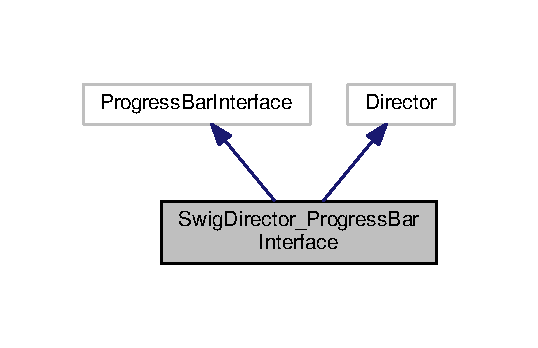
\includegraphics[width=258pt]{classSwigDirector__ProgressBarInterface__inherit__graph}
\end{center}
\end{figure}


Collaboration diagram for Swig\+Director\+\_\+\+Progress\+Bar\+Interface\+:
\nopagebreak
\begin{figure}[H]
\begin{center}
\leavevmode
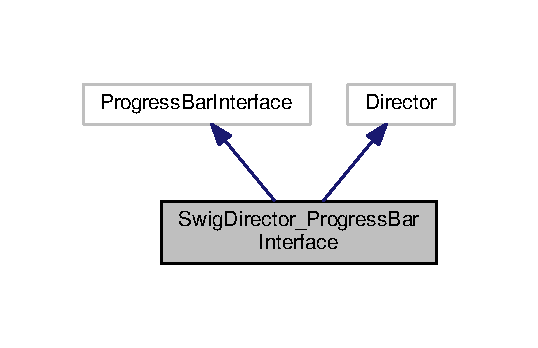
\includegraphics[width=258pt]{classSwigDirector__ProgressBarInterface__coll__graph}
\end{center}
\end{figure}
\subsection*{Public Member Functions}
\begin{DoxyCompactItemize}
\item 
\hyperlink{classSwigDirector__ProgressBarInterface_a24add52bac381bb2d0b2a01b09bd2a4f}{Swig\+Director\+\_\+\+Progress\+Bar\+Interface} (Py\+Object $\ast$self)
\item 
virtual void \hyperlink{classSwigDirector__ProgressBarInterface_a50f5d7778022e27d2f9dfa0b79e84dce}{show} (float percent)
\item 
virtual \hyperlink{classSwigDirector__ProgressBarInterface_a98e8dbc1e4b81ad2c0b8ea1ac2006dc3}{$\sim$\+Swig\+Director\+\_\+\+Progress\+Bar\+Interface} ()
\item 
bool \hyperlink{classSwigDirector__ProgressBarInterface_aca008c5d9c4dafd39fd494c6e060a5e4}{swig\+\_\+get\+\_\+inner} (const char $\ast$swig\+\_\+protected\+\_\+method\+\_\+name) const 
\item 
void \hyperlink{classSwigDirector__ProgressBarInterface_a9efd6adb1d3e2286ea9e4ac6487b5e79}{swig\+\_\+set\+\_\+inner} (const char $\ast$swig\+\_\+protected\+\_\+method\+\_\+name, bool val) const 
\end{DoxyCompactItemize}


\subsection{Constructor \& Destructor Documentation}
\hypertarget{classSwigDirector__ProgressBarInterface_a24add52bac381bb2d0b2a01b09bd2a4f}{\index{Swig\+Director\+\_\+\+Progress\+Bar\+Interface@{Swig\+Director\+\_\+\+Progress\+Bar\+Interface}!Swig\+Director\+\_\+\+Progress\+Bar\+Interface@{Swig\+Director\+\_\+\+Progress\+Bar\+Interface}}
\index{Swig\+Director\+\_\+\+Progress\+Bar\+Interface@{Swig\+Director\+\_\+\+Progress\+Bar\+Interface}!Swig\+Director\+\_\+\+Progress\+Bar\+Interface@{Swig\+Director\+\_\+\+Progress\+Bar\+Interface}}
\subsubsection[{Swig\+Director\+\_\+\+Progress\+Bar\+Interface}]{\setlength{\rightskip}{0pt plus 5cm}{\bf Swig\+Director\+\_\+\+Progress\+Bar\+Interface} (
\begin{DoxyParamCaption}
\item[{Py\+Object $\ast$}]{self}
\end{DoxyParamCaption}
)}}\label{classSwigDirector__ProgressBarInterface_a24add52bac381bb2d0b2a01b09bd2a4f}
\hypertarget{classSwigDirector__ProgressBarInterface_a98e8dbc1e4b81ad2c0b8ea1ac2006dc3}{\index{Swig\+Director\+\_\+\+Progress\+Bar\+Interface@{Swig\+Director\+\_\+\+Progress\+Bar\+Interface}!````~Swig\+Director\+\_\+\+Progress\+Bar\+Interface@{$\sim$\+Swig\+Director\+\_\+\+Progress\+Bar\+Interface}}
\index{````~Swig\+Director\+\_\+\+Progress\+Bar\+Interface@{$\sim$\+Swig\+Director\+\_\+\+Progress\+Bar\+Interface}!Swig\+Director\+\_\+\+Progress\+Bar\+Interface@{Swig\+Director\+\_\+\+Progress\+Bar\+Interface}}
\subsubsection[{$\sim$\+Swig\+Director\+\_\+\+Progress\+Bar\+Interface}]{\setlength{\rightskip}{0pt plus 5cm}virtual $\sim${\bf Swig\+Director\+\_\+\+Progress\+Bar\+Interface} (
\begin{DoxyParamCaption}
{}
\end{DoxyParamCaption}
)\hspace{0.3cm}{\ttfamily [virtual]}}}\label{classSwigDirector__ProgressBarInterface_a98e8dbc1e4b81ad2c0b8ea1ac2006dc3}


\subsection{Member Function Documentation}
\hypertarget{classSwigDirector__ProgressBarInterface_a50f5d7778022e27d2f9dfa0b79e84dce}{\index{Swig\+Director\+\_\+\+Progress\+Bar\+Interface@{Swig\+Director\+\_\+\+Progress\+Bar\+Interface}!show@{show}}
\index{show@{show}!Swig\+Director\+\_\+\+Progress\+Bar\+Interface@{Swig\+Director\+\_\+\+Progress\+Bar\+Interface}}
\subsubsection[{show}]{\setlength{\rightskip}{0pt plus 5cm}virtual void show (
\begin{DoxyParamCaption}
\item[{float}]{percent}
\end{DoxyParamCaption}
)\hspace{0.3cm}{\ttfamily [virtual]}}}\label{classSwigDirector__ProgressBarInterface_a50f5d7778022e27d2f9dfa0b79e84dce}
\hypertarget{classSwigDirector__ProgressBarInterface_aca008c5d9c4dafd39fd494c6e060a5e4}{\index{Swig\+Director\+\_\+\+Progress\+Bar\+Interface@{Swig\+Director\+\_\+\+Progress\+Bar\+Interface}!swig\+\_\+get\+\_\+inner@{swig\+\_\+get\+\_\+inner}}
\index{swig\+\_\+get\+\_\+inner@{swig\+\_\+get\+\_\+inner}!Swig\+Director\+\_\+\+Progress\+Bar\+Interface@{Swig\+Director\+\_\+\+Progress\+Bar\+Interface}}
\subsubsection[{swig\+\_\+get\+\_\+inner}]{\setlength{\rightskip}{0pt plus 5cm}bool swig\+\_\+get\+\_\+inner (
\begin{DoxyParamCaption}
\item[{const char $\ast$}]{swig\+\_\+protected\+\_\+method\+\_\+name}
\end{DoxyParamCaption}
) const\hspace{0.3cm}{\ttfamily [inline]}}}\label{classSwigDirector__ProgressBarInterface_aca008c5d9c4dafd39fd494c6e060a5e4}
\hypertarget{classSwigDirector__ProgressBarInterface_a9efd6adb1d3e2286ea9e4ac6487b5e79}{\index{Swig\+Director\+\_\+\+Progress\+Bar\+Interface@{Swig\+Director\+\_\+\+Progress\+Bar\+Interface}!swig\+\_\+set\+\_\+inner@{swig\+\_\+set\+\_\+inner}}
\index{swig\+\_\+set\+\_\+inner@{swig\+\_\+set\+\_\+inner}!Swig\+Director\+\_\+\+Progress\+Bar\+Interface@{Swig\+Director\+\_\+\+Progress\+Bar\+Interface}}
\subsubsection[{swig\+\_\+set\+\_\+inner}]{\setlength{\rightskip}{0pt plus 5cm}void swig\+\_\+set\+\_\+inner (
\begin{DoxyParamCaption}
\item[{const char $\ast$}]{swig\+\_\+protected\+\_\+method\+\_\+name, }
\item[{bool}]{val}
\end{DoxyParamCaption}
) const\hspace{0.3cm}{\ttfamily [inline]}}}\label{classSwigDirector__ProgressBarInterface_a9efd6adb1d3e2286ea9e4ac6487b5e79}


The documentation for this class was generated from the following file\+:\begin{DoxyCompactItemize}
\item 
\hyperlink{swig__fnmPYTHON__wrap_8h}{swig\+\_\+fnm\+P\+Y\+T\+H\+O\+N\+\_\+wrap.\+h}\end{DoxyCompactItemize}

\hypertarget{structfnm_1_1sysparm__t}{\section{sysparm\+\_\+t$<$ T $>$ Struct Template Reference}
\label{structfnm_1_1sysparm__t}\index{sysparm\+\_\+t$<$ T $>$@{sysparm\+\_\+t$<$ T $>$}}
}


Sysparm structure.  




{\ttfamily \#include $<$fnm\+\_\+types.\+hpp$>$}

\subsection*{Public Attributes}
\begin{DoxyCompactItemize}
\item 
T \hyperlink{structfnm_1_1sysparm__t_a169228264adc1071b8585ae0c7f390cd}{c}
\begin{DoxyCompactList}\small\item\em Speed of sound. \end{DoxyCompactList}\item 
size\+\_\+t \hyperlink{structfnm_1_1sysparm__t_a676de84ecc719ad3223182fb136690af}{n\+Div\+W}
\begin{DoxyCompactList}\small\item\em Number of width abcissas. \end{DoxyCompactList}\item 
size\+\_\+t \hyperlink{structfnm_1_1sysparm__t_a26cce015a626b46108d07cdbab336011}{n\+Div\+H}
\begin{DoxyCompactList}\small\item\em Number of height abcissas. \end{DoxyCompactList}\end{DoxyCompactItemize}


\subsection{Detailed Description}
\subsubsection*{template$<$class T$>$struct fnm\+::sysparm\+\_\+t$<$ T $>$}

Sysparm structure. 

A structure containing global simulation parameters 

\subsection{Member Data Documentation}
\hypertarget{structfnm_1_1sysparm__t_a169228264adc1071b8585ae0c7f390cd}{\index{fnm\+::sysparm\+\_\+t@{fnm\+::sysparm\+\_\+t}!c@{c}}
\index{c@{c}!fnm\+::sysparm\+\_\+t@{fnm\+::sysparm\+\_\+t}}
\subsubsection[{c}]{\setlength{\rightskip}{0pt plus 5cm}T c}}\label{structfnm_1_1sysparm__t_a169228264adc1071b8585ae0c7f390cd}


Speed of sound. 

\hypertarget{structfnm_1_1sysparm__t_a26cce015a626b46108d07cdbab336011}{\index{fnm\+::sysparm\+\_\+t@{fnm\+::sysparm\+\_\+t}!n\+Div\+H@{n\+Div\+H}}
\index{n\+Div\+H@{n\+Div\+H}!fnm\+::sysparm\+\_\+t@{fnm\+::sysparm\+\_\+t}}
\subsubsection[{n\+Div\+H}]{\setlength{\rightskip}{0pt plus 5cm}size\+\_\+t n\+Div\+H}}\label{structfnm_1_1sysparm__t_a26cce015a626b46108d07cdbab336011}


Number of height abcissas. 

\hypertarget{structfnm_1_1sysparm__t_a676de84ecc719ad3223182fb136690af}{\index{fnm\+::sysparm\+\_\+t@{fnm\+::sysparm\+\_\+t}!n\+Div\+W@{n\+Div\+W}}
\index{n\+Div\+W@{n\+Div\+W}!fnm\+::sysparm\+\_\+t@{fnm\+::sysparm\+\_\+t}}
\subsubsection[{n\+Div\+W}]{\setlength{\rightskip}{0pt plus 5cm}size\+\_\+t n\+Div\+W}}\label{structfnm_1_1sysparm__t_a676de84ecc719ad3223182fb136690af}


Number of width abcissas. 



The documentation for this struct was generated from the following file\+:\begin{DoxyCompactItemize}
\item 
fnm/\hyperlink{fnm__types_8hpp}{fnm\+\_\+types.\+hpp}\end{DoxyCompactItemize}

\chapter{File Documentation}
\hypertarget{config_8h}{\section{config.\+h File Reference}
\label{config_8h}\index{config.\+h@{config.\+h}}
}


Auto-\/generated configuration file.  


This graph shows which files directly or indirectly include this file\+:\nopagebreak
\begin{figure}[H]
\begin{center}
\leavevmode
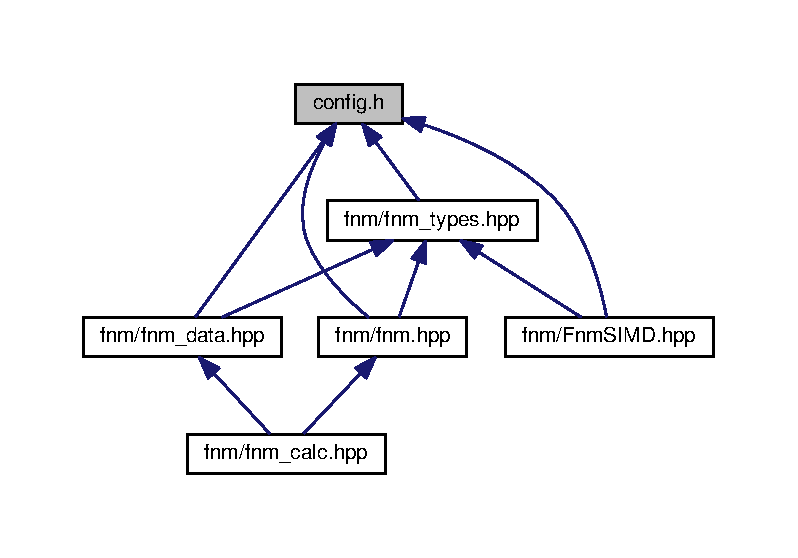
\includegraphics[width=350pt]{config_8h__dep__incl}
\end{center}
\end{figure}
\subsection*{Macros}
\begin{DoxyCompactItemize}
\item 
\#define \hyperlink{config_8h_acf71b36fdd29bd9ef6709cecac0536d2}{H\+A\+V\+E\+\_\+\+P\+T\+H\+R\+E\+A\+D\+\_\+\+H}~1
\item 
\#define \hyperlink{config_8h_aeab812b8a5539800d906e8c66fdeff07}{H\+A\+V\+E\+\_\+\+T\+H\+R\+E\+A\+D}~1
\item 
\#define \hyperlink{config_8h_aa2b4ec58d136b55d98135c44a4420bad}{N\+\_\+\+M\+A\+X\+\_\+\+T\+H\+R\+E\+A\+D\+S}~8
\end{DoxyCompactItemize}


\subsection{Detailed Description}
Auto-\/generated configuration file. 

\begin{DoxyAuthor}{Author}
Jens Munk Hansen \href{mailto:jens.munk.hansen@gmai.com}{\tt jens.\+munk.\+hansen@gmai.\+com} 
\end{DoxyAuthor}
\begin{DoxyDate}{Date}
Tue Apr 29 19\+:46\+:27 2014 
\end{DoxyDate}


\subsection{Macro Definition Documentation}
\hypertarget{config_8h_acf71b36fdd29bd9ef6709cecac0536d2}{\index{config.\+h@{config.\+h}!H\+A\+V\+E\+\_\+\+P\+T\+H\+R\+E\+A\+D\+\_\+\+H@{H\+A\+V\+E\+\_\+\+P\+T\+H\+R\+E\+A\+D\+\_\+\+H}}
\index{H\+A\+V\+E\+\_\+\+P\+T\+H\+R\+E\+A\+D\+\_\+\+H@{H\+A\+V\+E\+\_\+\+P\+T\+H\+R\+E\+A\+D\+\_\+\+H}!config.\+h@{config.\+h}}
\subsubsection[{H\+A\+V\+E\+\_\+\+P\+T\+H\+R\+E\+A\+D\+\_\+\+H}]{\setlength{\rightskip}{0pt plus 5cm}\#define H\+A\+V\+E\+\_\+\+P\+T\+H\+R\+E\+A\+D\+\_\+\+H~1}}\label{config_8h_acf71b36fdd29bd9ef6709cecac0536d2}
\hypertarget{config_8h_aeab812b8a5539800d906e8c66fdeff07}{\index{config.\+h@{config.\+h}!H\+A\+V\+E\+\_\+\+T\+H\+R\+E\+A\+D@{H\+A\+V\+E\+\_\+\+T\+H\+R\+E\+A\+D}}
\index{H\+A\+V\+E\+\_\+\+T\+H\+R\+E\+A\+D@{H\+A\+V\+E\+\_\+\+T\+H\+R\+E\+A\+D}!config.\+h@{config.\+h}}
\subsubsection[{H\+A\+V\+E\+\_\+\+T\+H\+R\+E\+A\+D}]{\setlength{\rightskip}{0pt plus 5cm}\#define H\+A\+V\+E\+\_\+\+T\+H\+R\+E\+A\+D~1}}\label{config_8h_aeab812b8a5539800d906e8c66fdeff07}
\hypertarget{config_8h_aa2b4ec58d136b55d98135c44a4420bad}{\index{config.\+h@{config.\+h}!N\+\_\+\+M\+A\+X\+\_\+\+T\+H\+R\+E\+A\+D\+S@{N\+\_\+\+M\+A\+X\+\_\+\+T\+H\+R\+E\+A\+D\+S}}
\index{N\+\_\+\+M\+A\+X\+\_\+\+T\+H\+R\+E\+A\+D\+S@{N\+\_\+\+M\+A\+X\+\_\+\+T\+H\+R\+E\+A\+D\+S}!config.\+h@{config.\+h}}
\subsubsection[{N\+\_\+\+M\+A\+X\+\_\+\+T\+H\+R\+E\+A\+D\+S}]{\setlength{\rightskip}{0pt plus 5cm}\#define N\+\_\+\+M\+A\+X\+\_\+\+T\+H\+R\+E\+A\+D\+S~8}}\label{config_8h_aa2b4ec58d136b55d98135c44a4420bad}

\hypertarget{fnm__export_8h}{\section{fnm\+\_\+export.\+h File Reference}
\label{fnm__export_8h}\index{fnm\+\_\+export.\+h@{fnm\+\_\+export.\+h}}
}
This graph shows which files directly or indirectly include this file\+:\nopagebreak
\begin{figure}[H]
\begin{center}
\leavevmode
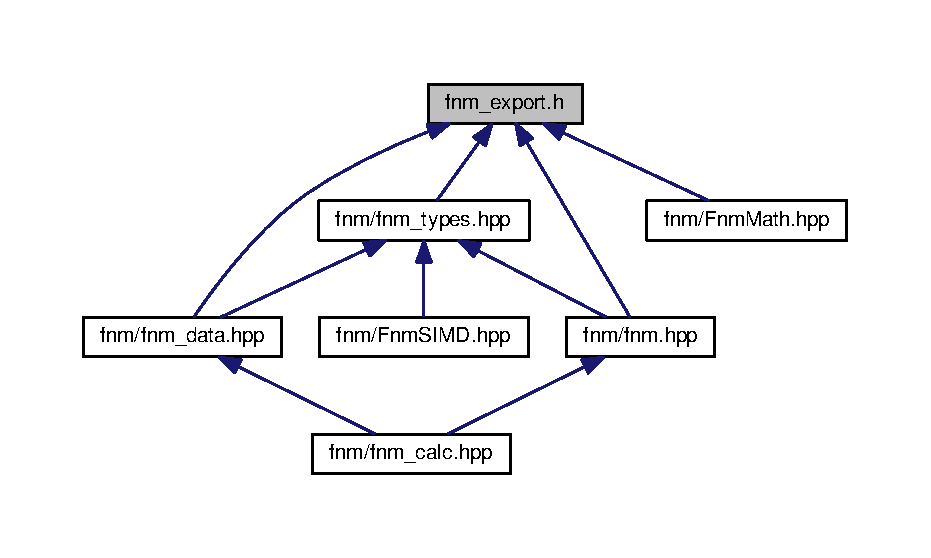
\includegraphics[width=350pt]{fnm__export_8h__dep__incl}
\end{center}
\end{figure}
\subsection*{Macros}
\begin{DoxyCompactItemize}
\item 
\#define \hyperlink{fnm__export_8h_a3ff7f8e85834af476dd033ada79d8790}{F\+N\+M\+\_\+\+E\+X\+P\+O\+R\+T}
\item 
\#define \hyperlink{fnm__export_8h_affaa1420e4dc887bc24274ff1c58ef82}{F\+N\+M\+\_\+\+N\+O\+\_\+\+E\+X\+P\+O\+R\+T}
\item 
\#define \hyperlink{fnm__export_8h_a36319a0b3f1bc150fc609be352d27341}{F\+N\+M\+\_\+\+D\+E\+P\+R\+E\+C\+A\+T\+E\+D}~\+\_\+\+\_\+attribute\+\_\+\+\_\+ ((\+\_\+\+\_\+deprecated\+\_\+\+\_\+))
\item 
\#define \hyperlink{fnm__export_8h_a562b6bb35ffd4e3d7bacb2a38df7bf90}{F\+N\+M\+\_\+\+D\+E\+P\+R\+E\+C\+A\+T\+E\+D\+\_\+\+E\+X\+P\+O\+R\+T}~\hyperlink{fnm__export_8h_a3ff7f8e85834af476dd033ada79d8790}{F\+N\+M\+\_\+\+E\+X\+P\+O\+R\+T} \hyperlink{fnm__export_8h_a36319a0b3f1bc150fc609be352d27341}{F\+N\+M\+\_\+\+D\+E\+P\+R\+E\+C\+A\+T\+E\+D}
\item 
\#define \hyperlink{fnm__export_8h_a8d0febf1f1658885b17af62a4bd4bc1c}{F\+N\+M\+\_\+\+D\+E\+P\+R\+E\+C\+A\+T\+E\+D\+\_\+\+N\+O\+\_\+\+E\+X\+P\+O\+R\+T}~\hyperlink{fnm__export_8h_affaa1420e4dc887bc24274ff1c58ef82}{F\+N\+M\+\_\+\+N\+O\+\_\+\+E\+X\+P\+O\+R\+T} \hyperlink{fnm__export_8h_a36319a0b3f1bc150fc609be352d27341}{F\+N\+M\+\_\+\+D\+E\+P\+R\+E\+C\+A\+T\+E\+D}
\item 
\#define \hyperlink{fnm__export_8h_ad1bbfc048f115ce6acd8245fa2466eb3}{D\+E\+F\+I\+N\+E\+\_\+\+N\+O\+\_\+\+D\+E\+P\+R\+E\+C\+A\+T\+E\+D}~0
\end{DoxyCompactItemize}


\subsection{Macro Definition Documentation}
\hypertarget{fnm__export_8h_ad1bbfc048f115ce6acd8245fa2466eb3}{\index{fnm\+\_\+export.\+h@{fnm\+\_\+export.\+h}!D\+E\+F\+I\+N\+E\+\_\+\+N\+O\+\_\+\+D\+E\+P\+R\+E\+C\+A\+T\+E\+D@{D\+E\+F\+I\+N\+E\+\_\+\+N\+O\+\_\+\+D\+E\+P\+R\+E\+C\+A\+T\+E\+D}}
\index{D\+E\+F\+I\+N\+E\+\_\+\+N\+O\+\_\+\+D\+E\+P\+R\+E\+C\+A\+T\+E\+D@{D\+E\+F\+I\+N\+E\+\_\+\+N\+O\+\_\+\+D\+E\+P\+R\+E\+C\+A\+T\+E\+D}!fnm\+\_\+export.\+h@{fnm\+\_\+export.\+h}}
\subsubsection[{D\+E\+F\+I\+N\+E\+\_\+\+N\+O\+\_\+\+D\+E\+P\+R\+E\+C\+A\+T\+E\+D}]{\setlength{\rightskip}{0pt plus 5cm}\#define D\+E\+F\+I\+N\+E\+\_\+\+N\+O\+\_\+\+D\+E\+P\+R\+E\+C\+A\+T\+E\+D~0}}\label{fnm__export_8h_ad1bbfc048f115ce6acd8245fa2466eb3}
\hypertarget{fnm__export_8h_a36319a0b3f1bc150fc609be352d27341}{\index{fnm\+\_\+export.\+h@{fnm\+\_\+export.\+h}!F\+N\+M\+\_\+\+D\+E\+P\+R\+E\+C\+A\+T\+E\+D@{F\+N\+M\+\_\+\+D\+E\+P\+R\+E\+C\+A\+T\+E\+D}}
\index{F\+N\+M\+\_\+\+D\+E\+P\+R\+E\+C\+A\+T\+E\+D@{F\+N\+M\+\_\+\+D\+E\+P\+R\+E\+C\+A\+T\+E\+D}!fnm\+\_\+export.\+h@{fnm\+\_\+export.\+h}}
\subsubsection[{F\+N\+M\+\_\+\+D\+E\+P\+R\+E\+C\+A\+T\+E\+D}]{\setlength{\rightskip}{0pt plus 5cm}\#define F\+N\+M\+\_\+\+D\+E\+P\+R\+E\+C\+A\+T\+E\+D~\+\_\+\+\_\+attribute\+\_\+\+\_\+ ((\+\_\+\+\_\+deprecated\+\_\+\+\_\+))}}\label{fnm__export_8h_a36319a0b3f1bc150fc609be352d27341}
\hypertarget{fnm__export_8h_a562b6bb35ffd4e3d7bacb2a38df7bf90}{\index{fnm\+\_\+export.\+h@{fnm\+\_\+export.\+h}!F\+N\+M\+\_\+\+D\+E\+P\+R\+E\+C\+A\+T\+E\+D\+\_\+\+E\+X\+P\+O\+R\+T@{F\+N\+M\+\_\+\+D\+E\+P\+R\+E\+C\+A\+T\+E\+D\+\_\+\+E\+X\+P\+O\+R\+T}}
\index{F\+N\+M\+\_\+\+D\+E\+P\+R\+E\+C\+A\+T\+E\+D\+\_\+\+E\+X\+P\+O\+R\+T@{F\+N\+M\+\_\+\+D\+E\+P\+R\+E\+C\+A\+T\+E\+D\+\_\+\+E\+X\+P\+O\+R\+T}!fnm\+\_\+export.\+h@{fnm\+\_\+export.\+h}}
\subsubsection[{F\+N\+M\+\_\+\+D\+E\+P\+R\+E\+C\+A\+T\+E\+D\+\_\+\+E\+X\+P\+O\+R\+T}]{\setlength{\rightskip}{0pt plus 5cm}\#define F\+N\+M\+\_\+\+D\+E\+P\+R\+E\+C\+A\+T\+E\+D\+\_\+\+E\+X\+P\+O\+R\+T~{\bf F\+N\+M\+\_\+\+E\+X\+P\+O\+R\+T} {\bf F\+N\+M\+\_\+\+D\+E\+P\+R\+E\+C\+A\+T\+E\+D}}}\label{fnm__export_8h_a562b6bb35ffd4e3d7bacb2a38df7bf90}
\hypertarget{fnm__export_8h_a8d0febf1f1658885b17af62a4bd4bc1c}{\index{fnm\+\_\+export.\+h@{fnm\+\_\+export.\+h}!F\+N\+M\+\_\+\+D\+E\+P\+R\+E\+C\+A\+T\+E\+D\+\_\+\+N\+O\+\_\+\+E\+X\+P\+O\+R\+T@{F\+N\+M\+\_\+\+D\+E\+P\+R\+E\+C\+A\+T\+E\+D\+\_\+\+N\+O\+\_\+\+E\+X\+P\+O\+R\+T}}
\index{F\+N\+M\+\_\+\+D\+E\+P\+R\+E\+C\+A\+T\+E\+D\+\_\+\+N\+O\+\_\+\+E\+X\+P\+O\+R\+T@{F\+N\+M\+\_\+\+D\+E\+P\+R\+E\+C\+A\+T\+E\+D\+\_\+\+N\+O\+\_\+\+E\+X\+P\+O\+R\+T}!fnm\+\_\+export.\+h@{fnm\+\_\+export.\+h}}
\subsubsection[{F\+N\+M\+\_\+\+D\+E\+P\+R\+E\+C\+A\+T\+E\+D\+\_\+\+N\+O\+\_\+\+E\+X\+P\+O\+R\+T}]{\setlength{\rightskip}{0pt plus 5cm}\#define F\+N\+M\+\_\+\+D\+E\+P\+R\+E\+C\+A\+T\+E\+D\+\_\+\+N\+O\+\_\+\+E\+X\+P\+O\+R\+T~{\bf F\+N\+M\+\_\+\+N\+O\+\_\+\+E\+X\+P\+O\+R\+T} {\bf F\+N\+M\+\_\+\+D\+E\+P\+R\+E\+C\+A\+T\+E\+D}}}\label{fnm__export_8h_a8d0febf1f1658885b17af62a4bd4bc1c}
\hypertarget{fnm__export_8h_a3ff7f8e85834af476dd033ada79d8790}{\index{fnm\+\_\+export.\+h@{fnm\+\_\+export.\+h}!F\+N\+M\+\_\+\+E\+X\+P\+O\+R\+T@{F\+N\+M\+\_\+\+E\+X\+P\+O\+R\+T}}
\index{F\+N\+M\+\_\+\+E\+X\+P\+O\+R\+T@{F\+N\+M\+\_\+\+E\+X\+P\+O\+R\+T}!fnm\+\_\+export.\+h@{fnm\+\_\+export.\+h}}
\subsubsection[{F\+N\+M\+\_\+\+E\+X\+P\+O\+R\+T}]{\setlength{\rightskip}{0pt plus 5cm}\#define F\+N\+M\+\_\+\+E\+X\+P\+O\+R\+T}}\label{fnm__export_8h_a3ff7f8e85834af476dd033ada79d8790}
\hypertarget{fnm__export_8h_affaa1420e4dc887bc24274ff1c58ef82}{\index{fnm\+\_\+export.\+h@{fnm\+\_\+export.\+h}!F\+N\+M\+\_\+\+N\+O\+\_\+\+E\+X\+P\+O\+R\+T@{F\+N\+M\+\_\+\+N\+O\+\_\+\+E\+X\+P\+O\+R\+T}}
\index{F\+N\+M\+\_\+\+N\+O\+\_\+\+E\+X\+P\+O\+R\+T@{F\+N\+M\+\_\+\+N\+O\+\_\+\+E\+X\+P\+O\+R\+T}!fnm\+\_\+export.\+h@{fnm\+\_\+export.\+h}}
\subsubsection[{F\+N\+M\+\_\+\+N\+O\+\_\+\+E\+X\+P\+O\+R\+T}]{\setlength{\rightskip}{0pt plus 5cm}\#define F\+N\+M\+\_\+\+N\+O\+\_\+\+E\+X\+P\+O\+R\+T}}\label{fnm__export_8h_affaa1420e4dc887bc24274ff1c58ef82}

\hypertarget{swig__fnmPYTHON__wrap_8h}{\section{swig\+\_\+fnm\+P\+Y\+T\+H\+O\+N\+\_\+wrap.\+h File Reference}
\label{swig__fnmPYTHON__wrap_8h}\index{swig\+\_\+fnm\+P\+Y\+T\+H\+O\+N\+\_\+wrap.\+h@{swig\+\_\+fnm\+P\+Y\+T\+H\+O\+N\+\_\+wrap.\+h}}
}
{\ttfamily \#include $<$map$>$}\\*
{\ttfamily \#include $<$string$>$}\\*
Include dependency graph for swig\+\_\+fnm\+P\+Y\+T\+H\+O\+N\+\_\+wrap.\+h\+:
\nopagebreak
\begin{figure}[H]
\begin{center}
\leavevmode
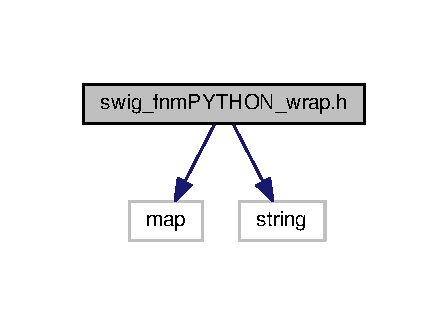
\includegraphics[width=215pt]{swig__fnmPYTHON__wrap_8h__incl}
\end{center}
\end{figure}
\subsection*{Classes}
\begin{DoxyCompactItemize}
\item 
class \hyperlink{classSwigDirector__ProgressBarInterface}{Swig\+Director\+\_\+\+Progress\+Bar\+Interface}
\end{DoxyCompactItemize}

\hypertarget{VersionInfo__Fnm_8h}{\section{Version\+Info\+\_\+\+Fnm.\+h File Reference}
\label{VersionInfo__Fnm_8h}\index{Version\+Info\+\_\+\+Fnm.\+h@{Version\+Info\+\_\+\+Fnm.\+h}}
}
\subsection*{Macros}
\begin{DoxyCompactItemize}
\item 
\#define \hyperlink{VersionInfo__Fnm_8h_a7dddbf944927a0b568923b796544b741}{P\+R\+O\+D\+U\+C\+T\+\_\+\+V\+E\+R\+S\+I\+O\+N\+\_\+\+M\+A\+J\+O\+R}~1
\item 
\#define \hyperlink{VersionInfo__Fnm_8h_a8b5c6dbae27886f06160455309d6783e}{P\+R\+O\+D\+U\+C\+T\+\_\+\+V\+E\+R\+S\+I\+O\+N\+\_\+\+M\+I\+N\+O\+R}~7
\item 
\#define \hyperlink{VersionInfo__Fnm_8h_acf6ca1bf587683c06f7e8d8bca654165}{P\+R\+O\+D\+U\+C\+T\+\_\+\+V\+E\+R\+S\+I\+O\+N\+\_\+\+P\+A\+T\+C\+H}~0
\item 
\#define \hyperlink{VersionInfo__Fnm_8h_a966f8186761e4df19d4c448b48334f66}{P\+R\+O\+D\+U\+C\+T\+\_\+\+V\+E\+R\+S\+I\+O\+N\+\_\+\+B\+U\+I\+L\+D}~20161203103309
\item 
\#define \hyperlink{VersionInfo__Fnm_8h_ada233e5218c8390ac9aabdfe5c4ace6c}{F\+I\+L\+E\+\_\+\+V\+E\+R\+S\+I\+O\+N\+\_\+\+M\+A\+J\+O\+R}~1
\item 
\#define \hyperlink{VersionInfo__Fnm_8h_a4154d27e45371f29e70856f8e964b3a8}{F\+I\+L\+E\+\_\+\+V\+E\+R\+S\+I\+O\+N\+\_\+\+M\+I\+N\+O\+R}~7
\item 
\#define \hyperlink{VersionInfo__Fnm_8h_a21e59bc19f3a5135d3c2695d80310c49}{F\+I\+L\+E\+\_\+\+V\+E\+R\+S\+I\+O\+N\+\_\+\+P\+A\+T\+C\+H}~0
\item 
\#define \hyperlink{VersionInfo__Fnm_8h_a6e7becbd875795024785a0488b44c039}{F\+I\+L\+E\+\_\+\+V\+E\+R\+S\+I\+O\+N\+\_\+\+B\+U\+I\+L\+D}~20161203103309
\item 
\#define \hyperlink{VersionInfo__Fnm_8h_a5f9559eb94e5c47578772d064fe473aa}{\+\_\+\+\_\+\+T\+O\+\_\+\+S\+T\+R\+I\+N\+G\+\_\+\+I\+M\+P\+L}(x)~\#x
\item 
\#define \hyperlink{VersionInfo__Fnm_8h_a10ed390ab06d6472da1d49adfaa9d4ee}{\+\_\+\+\_\+\+T\+O\+\_\+\+S\+T\+R\+I\+N\+G}(x)~\hyperlink{VersionInfo__Fnm_8h_a5f9559eb94e5c47578772d064fe473aa}{\+\_\+\+\_\+\+T\+O\+\_\+\+S\+T\+R\+I\+N\+G\+\_\+\+I\+M\+P\+L}(x)
\item 
\#define \hyperlink{VersionInfo__Fnm_8h_a5244bf34593e1efc482243c06194eb5b}{P\+R\+O\+D\+U\+C\+T\+\_\+\+V\+E\+R\+S\+I\+O\+N\+\_\+\+M\+A\+J\+O\+R\+\_\+\+M\+I\+N\+O\+R\+\_\+\+S\+T\+R}~\hyperlink{VersionInfo__Fnm_8h_a10ed390ab06d6472da1d49adfaa9d4ee}{\+\_\+\+\_\+\+T\+O\+\_\+\+S\+T\+R\+I\+N\+G}(\hyperlink{VersionInfo__Fnm_8h_a7dddbf944927a0b568923b796544b741}{P\+R\+O\+D\+U\+C\+T\+\_\+\+V\+E\+R\+S\+I\+O\+N\+\_\+\+M\+A\+J\+O\+R}) \char`\"{}.\char`\"{} \hyperlink{VersionInfo__Fnm_8h_a10ed390ab06d6472da1d49adfaa9d4ee}{\+\_\+\+\_\+\+T\+O\+\_\+\+S\+T\+R\+I\+N\+G}(\hyperlink{VersionInfo__Fnm_8h_a8b5c6dbae27886f06160455309d6783e}{P\+R\+O\+D\+U\+C\+T\+\_\+\+V\+E\+R\+S\+I\+O\+N\+\_\+\+M\+I\+N\+O\+R})
\item 
\#define \hyperlink{VersionInfo__Fnm_8h_aed4f512b403d4365493d28abae5c26fe}{P\+R\+O\+D\+U\+C\+T\+\_\+\+V\+E\+R\+S\+I\+O\+N\+\_\+\+M\+A\+J\+O\+R\+\_\+\+M\+I\+N\+O\+R\+\_\+\+P\+A\+T\+C\+H\+\_\+\+S\+T\+R}~\hyperlink{VersionInfo__Fnm_8h_a5244bf34593e1efc482243c06194eb5b}{P\+R\+O\+D\+U\+C\+T\+\_\+\+V\+E\+R\+S\+I\+O\+N\+\_\+\+M\+A\+J\+O\+R\+\_\+\+M\+I\+N\+O\+R\+\_\+\+S\+T\+R} \char`\"{}.\char`\"{} \hyperlink{VersionInfo__Fnm_8h_a10ed390ab06d6472da1d49adfaa9d4ee}{\+\_\+\+\_\+\+T\+O\+\_\+\+S\+T\+R\+I\+N\+G}(\hyperlink{VersionInfo__Fnm_8h_acf6ca1bf587683c06f7e8d8bca654165}{P\+R\+O\+D\+U\+C\+T\+\_\+\+V\+E\+R\+S\+I\+O\+N\+\_\+\+P\+A\+T\+C\+H})
\item 
\#define \hyperlink{VersionInfo__Fnm_8h_a5e8203c1ca2075773af587228a6eb77a}{P\+R\+O\+D\+U\+C\+T\+\_\+\+V\+E\+R\+S\+I\+O\+N\+\_\+\+F\+U\+L\+L\+\_\+\+S\+T\+R}~\hyperlink{VersionInfo__Fnm_8h_aed4f512b403d4365493d28abae5c26fe}{P\+R\+O\+D\+U\+C\+T\+\_\+\+V\+E\+R\+S\+I\+O\+N\+\_\+\+M\+A\+J\+O\+R\+\_\+\+M\+I\+N\+O\+R\+\_\+\+P\+A\+T\+C\+H\+\_\+\+S\+T\+R} \char`\"{}.\char`\"{} \hyperlink{VersionInfo__Fnm_8h_a10ed390ab06d6472da1d49adfaa9d4ee}{\+\_\+\+\_\+\+T\+O\+\_\+\+S\+T\+R\+I\+N\+G}(\hyperlink{VersionInfo__Fnm_8h_a966f8186761e4df19d4c448b48334f66}{P\+R\+O\+D\+U\+C\+T\+\_\+\+V\+E\+R\+S\+I\+O\+N\+\_\+\+B\+U\+I\+L\+D})
\item 
\#define \hyperlink{VersionInfo__Fnm_8h_a7b62d663a09c73a380a6dc82a713d828}{P\+R\+O\+D\+U\+C\+T\+\_\+\+V\+E\+R\+S\+I\+O\+N\+\_\+\+R\+E\+S\+O\+U\+R\+C\+E}~\hyperlink{VersionInfo__Fnm_8h_a7dddbf944927a0b568923b796544b741}{P\+R\+O\+D\+U\+C\+T\+\_\+\+V\+E\+R\+S\+I\+O\+N\+\_\+\+M\+A\+J\+O\+R},\hyperlink{VersionInfo__Fnm_8h_a8b5c6dbae27886f06160455309d6783e}{P\+R\+O\+D\+U\+C\+T\+\_\+\+V\+E\+R\+S\+I\+O\+N\+\_\+\+M\+I\+N\+O\+R},\hyperlink{VersionInfo__Fnm_8h_acf6ca1bf587683c06f7e8d8bca654165}{P\+R\+O\+D\+U\+C\+T\+\_\+\+V\+E\+R\+S\+I\+O\+N\+\_\+\+P\+A\+T\+C\+H},\hyperlink{VersionInfo__Fnm_8h_a966f8186761e4df19d4c448b48334f66}{P\+R\+O\+D\+U\+C\+T\+\_\+\+V\+E\+R\+S\+I\+O\+N\+\_\+\+B\+U\+I\+L\+D}
\item 
\#define \hyperlink{VersionInfo__Fnm_8h_a57959092117790b22a118b662fbf72a8}{P\+R\+O\+D\+U\+C\+T\+\_\+\+V\+E\+R\+S\+I\+O\+N\+\_\+\+R\+E\+S\+O\+U\+R\+C\+E\+\_\+\+S\+T\+R}~\hyperlink{VersionInfo__Fnm_8h_a5e8203c1ca2075773af587228a6eb77a}{P\+R\+O\+D\+U\+C\+T\+\_\+\+V\+E\+R\+S\+I\+O\+N\+\_\+\+F\+U\+L\+L\+\_\+\+S\+T\+R} \char`\"{}\textbackslash{}0\char`\"{}
\item 
\#define \hyperlink{VersionInfo__Fnm_8h_a0d2250d51ca862cae226e45d7101f2b4}{F\+I\+L\+E\+\_\+\+V\+E\+R\+S\+I\+O\+N\+\_\+\+M\+A\+J\+O\+R\+\_\+\+M\+I\+N\+O\+R\+\_\+\+S\+T\+R}~\hyperlink{VersionInfo__Fnm_8h_a10ed390ab06d6472da1d49adfaa9d4ee}{\+\_\+\+\_\+\+T\+O\+\_\+\+S\+T\+R\+I\+N\+G}(\hyperlink{VersionInfo__Fnm_8h_ada233e5218c8390ac9aabdfe5c4ace6c}{F\+I\+L\+E\+\_\+\+V\+E\+R\+S\+I\+O\+N\+\_\+\+M\+A\+J\+O\+R}) \char`\"{}.\char`\"{} \hyperlink{VersionInfo__Fnm_8h_a10ed390ab06d6472da1d49adfaa9d4ee}{\+\_\+\+\_\+\+T\+O\+\_\+\+S\+T\+R\+I\+N\+G}(\hyperlink{VersionInfo__Fnm_8h_a4154d27e45371f29e70856f8e964b3a8}{F\+I\+L\+E\+\_\+\+V\+E\+R\+S\+I\+O\+N\+\_\+\+M\+I\+N\+O\+R})
\item 
\#define \hyperlink{VersionInfo__Fnm_8h_a6de204d2a6754b3a0205d9fbc0370170}{F\+I\+L\+E\+\_\+\+V\+E\+R\+S\+I\+O\+N\+\_\+\+M\+A\+J\+O\+R\+\_\+\+M\+I\+N\+O\+R\+\_\+\+P\+A\+T\+C\+H\+\_\+\+S\+T\+R}~\hyperlink{VersionInfo__Fnm_8h_a0d2250d51ca862cae226e45d7101f2b4}{F\+I\+L\+E\+\_\+\+V\+E\+R\+S\+I\+O\+N\+\_\+\+M\+A\+J\+O\+R\+\_\+\+M\+I\+N\+O\+R\+\_\+\+S\+T\+R} \char`\"{}.\char`\"{} \hyperlink{VersionInfo__Fnm_8h_a10ed390ab06d6472da1d49adfaa9d4ee}{\+\_\+\+\_\+\+T\+O\+\_\+\+S\+T\+R\+I\+N\+G}(\hyperlink{VersionInfo__Fnm_8h_a21e59bc19f3a5135d3c2695d80310c49}{F\+I\+L\+E\+\_\+\+V\+E\+R\+S\+I\+O\+N\+\_\+\+P\+A\+T\+C\+H})
\item 
\#define \hyperlink{VersionInfo__Fnm_8h_a84db7867f2aafba92def27b60c094f56}{F\+I\+L\+E\+\_\+\+V\+E\+R\+S\+I\+O\+N\+\_\+\+F\+U\+L\+L\+\_\+\+S\+T\+R}~\hyperlink{VersionInfo__Fnm_8h_a6de204d2a6754b3a0205d9fbc0370170}{F\+I\+L\+E\+\_\+\+V\+E\+R\+S\+I\+O\+N\+\_\+\+M\+A\+J\+O\+R\+\_\+\+M\+I\+N\+O\+R\+\_\+\+P\+A\+T\+C\+H\+\_\+\+S\+T\+R} \char`\"{}.\char`\"{} \hyperlink{VersionInfo__Fnm_8h_a10ed390ab06d6472da1d49adfaa9d4ee}{\+\_\+\+\_\+\+T\+O\+\_\+\+S\+T\+R\+I\+N\+G}(\hyperlink{VersionInfo__Fnm_8h_a6e7becbd875795024785a0488b44c039}{F\+I\+L\+E\+\_\+\+V\+E\+R\+S\+I\+O\+N\+\_\+\+B\+U\+I\+L\+D})
\item 
\#define \hyperlink{VersionInfo__Fnm_8h_ae56cfce950d59353f8e67f0a869efb72}{F\+I\+L\+E\+\_\+\+V\+E\+R\+S\+I\+O\+N\+\_\+\+R\+E\+S\+O\+U\+R\+C\+E}~\hyperlink{VersionInfo__Fnm_8h_ada233e5218c8390ac9aabdfe5c4ace6c}{F\+I\+L\+E\+\_\+\+V\+E\+R\+S\+I\+O\+N\+\_\+\+M\+A\+J\+O\+R},\hyperlink{VersionInfo__Fnm_8h_a4154d27e45371f29e70856f8e964b3a8}{F\+I\+L\+E\+\_\+\+V\+E\+R\+S\+I\+O\+N\+\_\+\+M\+I\+N\+O\+R},\hyperlink{VersionInfo__Fnm_8h_a21e59bc19f3a5135d3c2695d80310c49}{F\+I\+L\+E\+\_\+\+V\+E\+R\+S\+I\+O\+N\+\_\+\+P\+A\+T\+C\+H},\hyperlink{VersionInfo__Fnm_8h_a6e7becbd875795024785a0488b44c039}{F\+I\+L\+E\+\_\+\+V\+E\+R\+S\+I\+O\+N\+\_\+\+B\+U\+I\+L\+D}
\item 
\#define \hyperlink{VersionInfo__Fnm_8h_a93e5f89011381f51471951bb4ab75b61}{F\+I\+L\+E\+\_\+\+V\+E\+R\+S\+I\+O\+N\+\_\+\+R\+E\+S\+O\+U\+R\+C\+E\+\_\+\+S\+T\+R}~\hyperlink{VersionInfo__Fnm_8h_a84db7867f2aafba92def27b60c094f56}{F\+I\+L\+E\+\_\+\+V\+E\+R\+S\+I\+O\+N\+\_\+\+F\+U\+L\+L\+\_\+\+S\+T\+R} \char`\"{}\textbackslash{}0\char`\"{}
\item 
\#define \hyperlink{VersionInfo__Fnm_8h_aea1c4c3fd221563d7c147d69f0aa4b7e}{P\+R\+O\+D\+U\+C\+T\+\_\+\+I\+C\+O\+N}~\char`\"{}/home/jmh/github/sofus/product.\+ico\char`\"{}
\item 
\#define \hyperlink{VersionInfo__Fnm_8h_a2e4f1ae08b2ac2308b22060428c98365}{P\+R\+O\+D\+U\+C\+T\+\_\+\+C\+O\+M\+M\+E\+N\+T\+S}~\char`\"{}Fnm v1.\+7\textbackslash{}0\char`\"{}
\item 
\#define \hyperlink{VersionInfo__Fnm_8h_a000a2fee862fab28140b6face0c12f8a}{P\+R\+O\+D\+U\+C\+T\+\_\+\+C\+O\+M\+P\+A\+N\+Y\+\_\+\+N\+A\+M\+E}~\char`\"{}\textbackslash{}0\char`\"{}
\item 
\#define \hyperlink{VersionInfo__Fnm_8h_a605560dc4b96a63a8ad22c7e87abc3be}{P\+R\+O\+D\+U\+C\+T\+\_\+\+C\+O\+M\+P\+A\+N\+Y\+\_\+\+C\+O\+P\+Y\+R\+I\+G\+H\+T}~\char`\"{} (C) Copyright 2016\textbackslash{}0\char`\"{}
\item 
\#define \hyperlink{VersionInfo__Fnm_8h_a337015d4c3f0a26d70924bc14743f683}{P\+R\+O\+D\+U\+C\+T\+\_\+\+F\+I\+L\+E\+\_\+\+D\+E\+S\+C\+R\+I\+P\+T\+I\+O\+N}~\char`\"{}Fnm\textbackslash{}0\char`\"{}
\item 
\#define \hyperlink{VersionInfo__Fnm_8h_a6b70c088a3a41ee19acc34a285ac2940}{P\+R\+O\+D\+U\+C\+T\+\_\+\+I\+N\+T\+E\+R\+N\+A\+L\+\_\+\+N\+A\+M\+E}~\char`\"{}Fnm\textbackslash{}0\char`\"{}
\item 
\#define \hyperlink{VersionInfo__Fnm_8h_ac04eff0a6312fcf0f9d8f317f3c5382b}{P\+R\+O\+D\+U\+C\+T\+\_\+\+O\+R\+I\+G\+I\+N\+A\+L\+\_\+\+F\+I\+L\+E\+N\+A\+M\+E}~\char`\"{}Fnm\textbackslash{}0\char`\"{}
\item 
\#define \hyperlink{VersionInfo__Fnm_8h_a62b539974094d0751b680791b74bdbf0}{P\+R\+O\+D\+U\+C\+T\+\_\+\+B\+U\+N\+D\+L\+E}~\char`\"{}Fnm\textbackslash{}0\char`\"{}
\end{DoxyCompactItemize}


\subsection{Macro Definition Documentation}
\hypertarget{VersionInfo__Fnm_8h_a10ed390ab06d6472da1d49adfaa9d4ee}{\index{Version\+Info\+\_\+\+Fnm.\+h@{Version\+Info\+\_\+\+Fnm.\+h}!\+\_\+\+\_\+\+T\+O\+\_\+\+S\+T\+R\+I\+N\+G@{\+\_\+\+\_\+\+T\+O\+\_\+\+S\+T\+R\+I\+N\+G}}
\index{\+\_\+\+\_\+\+T\+O\+\_\+\+S\+T\+R\+I\+N\+G@{\+\_\+\+\_\+\+T\+O\+\_\+\+S\+T\+R\+I\+N\+G}!Version\+Info\+\_\+\+Fnm.\+h@{Version\+Info\+\_\+\+Fnm.\+h}}
\subsubsection[{\+\_\+\+\_\+\+T\+O\+\_\+\+S\+T\+R\+I\+N\+G}]{\setlength{\rightskip}{0pt plus 5cm}\#define \+\_\+\+\_\+\+T\+O\+\_\+\+S\+T\+R\+I\+N\+G(
\begin{DoxyParamCaption}
\item[{}]{x}
\end{DoxyParamCaption}
)~{\bf \+\_\+\+\_\+\+T\+O\+\_\+\+S\+T\+R\+I\+N\+G\+\_\+\+I\+M\+P\+L}(x)}}\label{VersionInfo__Fnm_8h_a10ed390ab06d6472da1d49adfaa9d4ee}
\hypertarget{VersionInfo__Fnm_8h_a5f9559eb94e5c47578772d064fe473aa}{\index{Version\+Info\+\_\+\+Fnm.\+h@{Version\+Info\+\_\+\+Fnm.\+h}!\+\_\+\+\_\+\+T\+O\+\_\+\+S\+T\+R\+I\+N\+G\+\_\+\+I\+M\+P\+L@{\+\_\+\+\_\+\+T\+O\+\_\+\+S\+T\+R\+I\+N\+G\+\_\+\+I\+M\+P\+L}}
\index{\+\_\+\+\_\+\+T\+O\+\_\+\+S\+T\+R\+I\+N\+G\+\_\+\+I\+M\+P\+L@{\+\_\+\+\_\+\+T\+O\+\_\+\+S\+T\+R\+I\+N\+G\+\_\+\+I\+M\+P\+L}!Version\+Info\+\_\+\+Fnm.\+h@{Version\+Info\+\_\+\+Fnm.\+h}}
\subsubsection[{\+\_\+\+\_\+\+T\+O\+\_\+\+S\+T\+R\+I\+N\+G\+\_\+\+I\+M\+P\+L}]{\setlength{\rightskip}{0pt plus 5cm}\#define \+\_\+\+\_\+\+T\+O\+\_\+\+S\+T\+R\+I\+N\+G\+\_\+\+I\+M\+P\+L(
\begin{DoxyParamCaption}
\item[{}]{x}
\end{DoxyParamCaption}
)~\#x}}\label{VersionInfo__Fnm_8h_a5f9559eb94e5c47578772d064fe473aa}
\hypertarget{VersionInfo__Fnm_8h_a6e7becbd875795024785a0488b44c039}{\index{Version\+Info\+\_\+\+Fnm.\+h@{Version\+Info\+\_\+\+Fnm.\+h}!F\+I\+L\+E\+\_\+\+V\+E\+R\+S\+I\+O\+N\+\_\+\+B\+U\+I\+L\+D@{F\+I\+L\+E\+\_\+\+V\+E\+R\+S\+I\+O\+N\+\_\+\+B\+U\+I\+L\+D}}
\index{F\+I\+L\+E\+\_\+\+V\+E\+R\+S\+I\+O\+N\+\_\+\+B\+U\+I\+L\+D@{F\+I\+L\+E\+\_\+\+V\+E\+R\+S\+I\+O\+N\+\_\+\+B\+U\+I\+L\+D}!Version\+Info\+\_\+\+Fnm.\+h@{Version\+Info\+\_\+\+Fnm.\+h}}
\subsubsection[{F\+I\+L\+E\+\_\+\+V\+E\+R\+S\+I\+O\+N\+\_\+\+B\+U\+I\+L\+D}]{\setlength{\rightskip}{0pt plus 5cm}\#define F\+I\+L\+E\+\_\+\+V\+E\+R\+S\+I\+O\+N\+\_\+\+B\+U\+I\+L\+D~20161203103309}}\label{VersionInfo__Fnm_8h_a6e7becbd875795024785a0488b44c039}
\hypertarget{VersionInfo__Fnm_8h_a84db7867f2aafba92def27b60c094f56}{\index{Version\+Info\+\_\+\+Fnm.\+h@{Version\+Info\+\_\+\+Fnm.\+h}!F\+I\+L\+E\+\_\+\+V\+E\+R\+S\+I\+O\+N\+\_\+\+F\+U\+L\+L\+\_\+\+S\+T\+R@{F\+I\+L\+E\+\_\+\+V\+E\+R\+S\+I\+O\+N\+\_\+\+F\+U\+L\+L\+\_\+\+S\+T\+R}}
\index{F\+I\+L\+E\+\_\+\+V\+E\+R\+S\+I\+O\+N\+\_\+\+F\+U\+L\+L\+\_\+\+S\+T\+R@{F\+I\+L\+E\+\_\+\+V\+E\+R\+S\+I\+O\+N\+\_\+\+F\+U\+L\+L\+\_\+\+S\+T\+R}!Version\+Info\+\_\+\+Fnm.\+h@{Version\+Info\+\_\+\+Fnm.\+h}}
\subsubsection[{F\+I\+L\+E\+\_\+\+V\+E\+R\+S\+I\+O\+N\+\_\+\+F\+U\+L\+L\+\_\+\+S\+T\+R}]{\setlength{\rightskip}{0pt plus 5cm}\#define F\+I\+L\+E\+\_\+\+V\+E\+R\+S\+I\+O\+N\+\_\+\+F\+U\+L\+L\+\_\+\+S\+T\+R~{\bf F\+I\+L\+E\+\_\+\+V\+E\+R\+S\+I\+O\+N\+\_\+\+M\+A\+J\+O\+R\+\_\+\+M\+I\+N\+O\+R\+\_\+\+P\+A\+T\+C\+H\+\_\+\+S\+T\+R} \char`\"{}.\char`\"{} {\bf \+\_\+\+\_\+\+T\+O\+\_\+\+S\+T\+R\+I\+N\+G}({\bf F\+I\+L\+E\+\_\+\+V\+E\+R\+S\+I\+O\+N\+\_\+\+B\+U\+I\+L\+D})}}\label{VersionInfo__Fnm_8h_a84db7867f2aafba92def27b60c094f56}
\hypertarget{VersionInfo__Fnm_8h_ada233e5218c8390ac9aabdfe5c4ace6c}{\index{Version\+Info\+\_\+\+Fnm.\+h@{Version\+Info\+\_\+\+Fnm.\+h}!F\+I\+L\+E\+\_\+\+V\+E\+R\+S\+I\+O\+N\+\_\+\+M\+A\+J\+O\+R@{F\+I\+L\+E\+\_\+\+V\+E\+R\+S\+I\+O\+N\+\_\+\+M\+A\+J\+O\+R}}
\index{F\+I\+L\+E\+\_\+\+V\+E\+R\+S\+I\+O\+N\+\_\+\+M\+A\+J\+O\+R@{F\+I\+L\+E\+\_\+\+V\+E\+R\+S\+I\+O\+N\+\_\+\+M\+A\+J\+O\+R}!Version\+Info\+\_\+\+Fnm.\+h@{Version\+Info\+\_\+\+Fnm.\+h}}
\subsubsection[{F\+I\+L\+E\+\_\+\+V\+E\+R\+S\+I\+O\+N\+\_\+\+M\+A\+J\+O\+R}]{\setlength{\rightskip}{0pt plus 5cm}\#define F\+I\+L\+E\+\_\+\+V\+E\+R\+S\+I\+O\+N\+\_\+\+M\+A\+J\+O\+R~1}}\label{VersionInfo__Fnm_8h_ada233e5218c8390ac9aabdfe5c4ace6c}
\hypertarget{VersionInfo__Fnm_8h_a6de204d2a6754b3a0205d9fbc0370170}{\index{Version\+Info\+\_\+\+Fnm.\+h@{Version\+Info\+\_\+\+Fnm.\+h}!F\+I\+L\+E\+\_\+\+V\+E\+R\+S\+I\+O\+N\+\_\+\+M\+A\+J\+O\+R\+\_\+\+M\+I\+N\+O\+R\+\_\+\+P\+A\+T\+C\+H\+\_\+\+S\+T\+R@{F\+I\+L\+E\+\_\+\+V\+E\+R\+S\+I\+O\+N\+\_\+\+M\+A\+J\+O\+R\+\_\+\+M\+I\+N\+O\+R\+\_\+\+P\+A\+T\+C\+H\+\_\+\+S\+T\+R}}
\index{F\+I\+L\+E\+\_\+\+V\+E\+R\+S\+I\+O\+N\+\_\+\+M\+A\+J\+O\+R\+\_\+\+M\+I\+N\+O\+R\+\_\+\+P\+A\+T\+C\+H\+\_\+\+S\+T\+R@{F\+I\+L\+E\+\_\+\+V\+E\+R\+S\+I\+O\+N\+\_\+\+M\+A\+J\+O\+R\+\_\+\+M\+I\+N\+O\+R\+\_\+\+P\+A\+T\+C\+H\+\_\+\+S\+T\+R}!Version\+Info\+\_\+\+Fnm.\+h@{Version\+Info\+\_\+\+Fnm.\+h}}
\subsubsection[{F\+I\+L\+E\+\_\+\+V\+E\+R\+S\+I\+O\+N\+\_\+\+M\+A\+J\+O\+R\+\_\+\+M\+I\+N\+O\+R\+\_\+\+P\+A\+T\+C\+H\+\_\+\+S\+T\+R}]{\setlength{\rightskip}{0pt plus 5cm}\#define F\+I\+L\+E\+\_\+\+V\+E\+R\+S\+I\+O\+N\+\_\+\+M\+A\+J\+O\+R\+\_\+\+M\+I\+N\+O\+R\+\_\+\+P\+A\+T\+C\+H\+\_\+\+S\+T\+R~{\bf F\+I\+L\+E\+\_\+\+V\+E\+R\+S\+I\+O\+N\+\_\+\+M\+A\+J\+O\+R\+\_\+\+M\+I\+N\+O\+R\+\_\+\+S\+T\+R} \char`\"{}.\char`\"{} {\bf \+\_\+\+\_\+\+T\+O\+\_\+\+S\+T\+R\+I\+N\+G}({\bf F\+I\+L\+E\+\_\+\+V\+E\+R\+S\+I\+O\+N\+\_\+\+P\+A\+T\+C\+H})}}\label{VersionInfo__Fnm_8h_a6de204d2a6754b3a0205d9fbc0370170}
\hypertarget{VersionInfo__Fnm_8h_a0d2250d51ca862cae226e45d7101f2b4}{\index{Version\+Info\+\_\+\+Fnm.\+h@{Version\+Info\+\_\+\+Fnm.\+h}!F\+I\+L\+E\+\_\+\+V\+E\+R\+S\+I\+O\+N\+\_\+\+M\+A\+J\+O\+R\+\_\+\+M\+I\+N\+O\+R\+\_\+\+S\+T\+R@{F\+I\+L\+E\+\_\+\+V\+E\+R\+S\+I\+O\+N\+\_\+\+M\+A\+J\+O\+R\+\_\+\+M\+I\+N\+O\+R\+\_\+\+S\+T\+R}}
\index{F\+I\+L\+E\+\_\+\+V\+E\+R\+S\+I\+O\+N\+\_\+\+M\+A\+J\+O\+R\+\_\+\+M\+I\+N\+O\+R\+\_\+\+S\+T\+R@{F\+I\+L\+E\+\_\+\+V\+E\+R\+S\+I\+O\+N\+\_\+\+M\+A\+J\+O\+R\+\_\+\+M\+I\+N\+O\+R\+\_\+\+S\+T\+R}!Version\+Info\+\_\+\+Fnm.\+h@{Version\+Info\+\_\+\+Fnm.\+h}}
\subsubsection[{F\+I\+L\+E\+\_\+\+V\+E\+R\+S\+I\+O\+N\+\_\+\+M\+A\+J\+O\+R\+\_\+\+M\+I\+N\+O\+R\+\_\+\+S\+T\+R}]{\setlength{\rightskip}{0pt plus 5cm}\#define F\+I\+L\+E\+\_\+\+V\+E\+R\+S\+I\+O\+N\+\_\+\+M\+A\+J\+O\+R\+\_\+\+M\+I\+N\+O\+R\+\_\+\+S\+T\+R~{\bf \+\_\+\+\_\+\+T\+O\+\_\+\+S\+T\+R\+I\+N\+G}({\bf F\+I\+L\+E\+\_\+\+V\+E\+R\+S\+I\+O\+N\+\_\+\+M\+A\+J\+O\+R}) \char`\"{}.\char`\"{} {\bf \+\_\+\+\_\+\+T\+O\+\_\+\+S\+T\+R\+I\+N\+G}({\bf F\+I\+L\+E\+\_\+\+V\+E\+R\+S\+I\+O\+N\+\_\+\+M\+I\+N\+O\+R})}}\label{VersionInfo__Fnm_8h_a0d2250d51ca862cae226e45d7101f2b4}
\hypertarget{VersionInfo__Fnm_8h_a4154d27e45371f29e70856f8e964b3a8}{\index{Version\+Info\+\_\+\+Fnm.\+h@{Version\+Info\+\_\+\+Fnm.\+h}!F\+I\+L\+E\+\_\+\+V\+E\+R\+S\+I\+O\+N\+\_\+\+M\+I\+N\+O\+R@{F\+I\+L\+E\+\_\+\+V\+E\+R\+S\+I\+O\+N\+\_\+\+M\+I\+N\+O\+R}}
\index{F\+I\+L\+E\+\_\+\+V\+E\+R\+S\+I\+O\+N\+\_\+\+M\+I\+N\+O\+R@{F\+I\+L\+E\+\_\+\+V\+E\+R\+S\+I\+O\+N\+\_\+\+M\+I\+N\+O\+R}!Version\+Info\+\_\+\+Fnm.\+h@{Version\+Info\+\_\+\+Fnm.\+h}}
\subsubsection[{F\+I\+L\+E\+\_\+\+V\+E\+R\+S\+I\+O\+N\+\_\+\+M\+I\+N\+O\+R}]{\setlength{\rightskip}{0pt plus 5cm}\#define F\+I\+L\+E\+\_\+\+V\+E\+R\+S\+I\+O\+N\+\_\+\+M\+I\+N\+O\+R~7}}\label{VersionInfo__Fnm_8h_a4154d27e45371f29e70856f8e964b3a8}
\hypertarget{VersionInfo__Fnm_8h_a21e59bc19f3a5135d3c2695d80310c49}{\index{Version\+Info\+\_\+\+Fnm.\+h@{Version\+Info\+\_\+\+Fnm.\+h}!F\+I\+L\+E\+\_\+\+V\+E\+R\+S\+I\+O\+N\+\_\+\+P\+A\+T\+C\+H@{F\+I\+L\+E\+\_\+\+V\+E\+R\+S\+I\+O\+N\+\_\+\+P\+A\+T\+C\+H}}
\index{F\+I\+L\+E\+\_\+\+V\+E\+R\+S\+I\+O\+N\+\_\+\+P\+A\+T\+C\+H@{F\+I\+L\+E\+\_\+\+V\+E\+R\+S\+I\+O\+N\+\_\+\+P\+A\+T\+C\+H}!Version\+Info\+\_\+\+Fnm.\+h@{Version\+Info\+\_\+\+Fnm.\+h}}
\subsubsection[{F\+I\+L\+E\+\_\+\+V\+E\+R\+S\+I\+O\+N\+\_\+\+P\+A\+T\+C\+H}]{\setlength{\rightskip}{0pt plus 5cm}\#define F\+I\+L\+E\+\_\+\+V\+E\+R\+S\+I\+O\+N\+\_\+\+P\+A\+T\+C\+H~0}}\label{VersionInfo__Fnm_8h_a21e59bc19f3a5135d3c2695d80310c49}
\hypertarget{VersionInfo__Fnm_8h_ae56cfce950d59353f8e67f0a869efb72}{\index{Version\+Info\+\_\+\+Fnm.\+h@{Version\+Info\+\_\+\+Fnm.\+h}!F\+I\+L\+E\+\_\+\+V\+E\+R\+S\+I\+O\+N\+\_\+\+R\+E\+S\+O\+U\+R\+C\+E@{F\+I\+L\+E\+\_\+\+V\+E\+R\+S\+I\+O\+N\+\_\+\+R\+E\+S\+O\+U\+R\+C\+E}}
\index{F\+I\+L\+E\+\_\+\+V\+E\+R\+S\+I\+O\+N\+\_\+\+R\+E\+S\+O\+U\+R\+C\+E@{F\+I\+L\+E\+\_\+\+V\+E\+R\+S\+I\+O\+N\+\_\+\+R\+E\+S\+O\+U\+R\+C\+E}!Version\+Info\+\_\+\+Fnm.\+h@{Version\+Info\+\_\+\+Fnm.\+h}}
\subsubsection[{F\+I\+L\+E\+\_\+\+V\+E\+R\+S\+I\+O\+N\+\_\+\+R\+E\+S\+O\+U\+R\+C\+E}]{\setlength{\rightskip}{0pt plus 5cm}\#define F\+I\+L\+E\+\_\+\+V\+E\+R\+S\+I\+O\+N\+\_\+\+R\+E\+S\+O\+U\+R\+C\+E~{\bf F\+I\+L\+E\+\_\+\+V\+E\+R\+S\+I\+O\+N\+\_\+\+M\+A\+J\+O\+R},{\bf F\+I\+L\+E\+\_\+\+V\+E\+R\+S\+I\+O\+N\+\_\+\+M\+I\+N\+O\+R},{\bf F\+I\+L\+E\+\_\+\+V\+E\+R\+S\+I\+O\+N\+\_\+\+P\+A\+T\+C\+H},{\bf F\+I\+L\+E\+\_\+\+V\+E\+R\+S\+I\+O\+N\+\_\+\+B\+U\+I\+L\+D}}}\label{VersionInfo__Fnm_8h_ae56cfce950d59353f8e67f0a869efb72}
\hypertarget{VersionInfo__Fnm_8h_a93e5f89011381f51471951bb4ab75b61}{\index{Version\+Info\+\_\+\+Fnm.\+h@{Version\+Info\+\_\+\+Fnm.\+h}!F\+I\+L\+E\+\_\+\+V\+E\+R\+S\+I\+O\+N\+\_\+\+R\+E\+S\+O\+U\+R\+C\+E\+\_\+\+S\+T\+R@{F\+I\+L\+E\+\_\+\+V\+E\+R\+S\+I\+O\+N\+\_\+\+R\+E\+S\+O\+U\+R\+C\+E\+\_\+\+S\+T\+R}}
\index{F\+I\+L\+E\+\_\+\+V\+E\+R\+S\+I\+O\+N\+\_\+\+R\+E\+S\+O\+U\+R\+C\+E\+\_\+\+S\+T\+R@{F\+I\+L\+E\+\_\+\+V\+E\+R\+S\+I\+O\+N\+\_\+\+R\+E\+S\+O\+U\+R\+C\+E\+\_\+\+S\+T\+R}!Version\+Info\+\_\+\+Fnm.\+h@{Version\+Info\+\_\+\+Fnm.\+h}}
\subsubsection[{F\+I\+L\+E\+\_\+\+V\+E\+R\+S\+I\+O\+N\+\_\+\+R\+E\+S\+O\+U\+R\+C\+E\+\_\+\+S\+T\+R}]{\setlength{\rightskip}{0pt plus 5cm}\#define F\+I\+L\+E\+\_\+\+V\+E\+R\+S\+I\+O\+N\+\_\+\+R\+E\+S\+O\+U\+R\+C\+E\+\_\+\+S\+T\+R~{\bf F\+I\+L\+E\+\_\+\+V\+E\+R\+S\+I\+O\+N\+\_\+\+F\+U\+L\+L\+\_\+\+S\+T\+R} \char`\"{}\textbackslash{}0\char`\"{}}}\label{VersionInfo__Fnm_8h_a93e5f89011381f51471951bb4ab75b61}
\hypertarget{VersionInfo__Fnm_8h_a62b539974094d0751b680791b74bdbf0}{\index{Version\+Info\+\_\+\+Fnm.\+h@{Version\+Info\+\_\+\+Fnm.\+h}!P\+R\+O\+D\+U\+C\+T\+\_\+\+B\+U\+N\+D\+L\+E@{P\+R\+O\+D\+U\+C\+T\+\_\+\+B\+U\+N\+D\+L\+E}}
\index{P\+R\+O\+D\+U\+C\+T\+\_\+\+B\+U\+N\+D\+L\+E@{P\+R\+O\+D\+U\+C\+T\+\_\+\+B\+U\+N\+D\+L\+E}!Version\+Info\+\_\+\+Fnm.\+h@{Version\+Info\+\_\+\+Fnm.\+h}}
\subsubsection[{P\+R\+O\+D\+U\+C\+T\+\_\+\+B\+U\+N\+D\+L\+E}]{\setlength{\rightskip}{0pt plus 5cm}\#define P\+R\+O\+D\+U\+C\+T\+\_\+\+B\+U\+N\+D\+L\+E~\char`\"{}Fnm\textbackslash{}0\char`\"{}}}\label{VersionInfo__Fnm_8h_a62b539974094d0751b680791b74bdbf0}
\hypertarget{VersionInfo__Fnm_8h_a2e4f1ae08b2ac2308b22060428c98365}{\index{Version\+Info\+\_\+\+Fnm.\+h@{Version\+Info\+\_\+\+Fnm.\+h}!P\+R\+O\+D\+U\+C\+T\+\_\+\+C\+O\+M\+M\+E\+N\+T\+S@{P\+R\+O\+D\+U\+C\+T\+\_\+\+C\+O\+M\+M\+E\+N\+T\+S}}
\index{P\+R\+O\+D\+U\+C\+T\+\_\+\+C\+O\+M\+M\+E\+N\+T\+S@{P\+R\+O\+D\+U\+C\+T\+\_\+\+C\+O\+M\+M\+E\+N\+T\+S}!Version\+Info\+\_\+\+Fnm.\+h@{Version\+Info\+\_\+\+Fnm.\+h}}
\subsubsection[{P\+R\+O\+D\+U\+C\+T\+\_\+\+C\+O\+M\+M\+E\+N\+T\+S}]{\setlength{\rightskip}{0pt plus 5cm}\#define P\+R\+O\+D\+U\+C\+T\+\_\+\+C\+O\+M\+M\+E\+N\+T\+S~\char`\"{}Fnm v1.\+7\textbackslash{}0\char`\"{}}}\label{VersionInfo__Fnm_8h_a2e4f1ae08b2ac2308b22060428c98365}
\hypertarget{VersionInfo__Fnm_8h_a605560dc4b96a63a8ad22c7e87abc3be}{\index{Version\+Info\+\_\+\+Fnm.\+h@{Version\+Info\+\_\+\+Fnm.\+h}!P\+R\+O\+D\+U\+C\+T\+\_\+\+C\+O\+M\+P\+A\+N\+Y\+\_\+\+C\+O\+P\+Y\+R\+I\+G\+H\+T@{P\+R\+O\+D\+U\+C\+T\+\_\+\+C\+O\+M\+P\+A\+N\+Y\+\_\+\+C\+O\+P\+Y\+R\+I\+G\+H\+T}}
\index{P\+R\+O\+D\+U\+C\+T\+\_\+\+C\+O\+M\+P\+A\+N\+Y\+\_\+\+C\+O\+P\+Y\+R\+I\+G\+H\+T@{P\+R\+O\+D\+U\+C\+T\+\_\+\+C\+O\+M\+P\+A\+N\+Y\+\_\+\+C\+O\+P\+Y\+R\+I\+G\+H\+T}!Version\+Info\+\_\+\+Fnm.\+h@{Version\+Info\+\_\+\+Fnm.\+h}}
\subsubsection[{P\+R\+O\+D\+U\+C\+T\+\_\+\+C\+O\+M\+P\+A\+N\+Y\+\_\+\+C\+O\+P\+Y\+R\+I\+G\+H\+T}]{\setlength{\rightskip}{0pt plus 5cm}\#define P\+R\+O\+D\+U\+C\+T\+\_\+\+C\+O\+M\+P\+A\+N\+Y\+\_\+\+C\+O\+P\+Y\+R\+I\+G\+H\+T~\char`\"{} (C) Copyright 2016\textbackslash{}0\char`\"{}}}\label{VersionInfo__Fnm_8h_a605560dc4b96a63a8ad22c7e87abc3be}
\hypertarget{VersionInfo__Fnm_8h_a000a2fee862fab28140b6face0c12f8a}{\index{Version\+Info\+\_\+\+Fnm.\+h@{Version\+Info\+\_\+\+Fnm.\+h}!P\+R\+O\+D\+U\+C\+T\+\_\+\+C\+O\+M\+P\+A\+N\+Y\+\_\+\+N\+A\+M\+E@{P\+R\+O\+D\+U\+C\+T\+\_\+\+C\+O\+M\+P\+A\+N\+Y\+\_\+\+N\+A\+M\+E}}
\index{P\+R\+O\+D\+U\+C\+T\+\_\+\+C\+O\+M\+P\+A\+N\+Y\+\_\+\+N\+A\+M\+E@{P\+R\+O\+D\+U\+C\+T\+\_\+\+C\+O\+M\+P\+A\+N\+Y\+\_\+\+N\+A\+M\+E}!Version\+Info\+\_\+\+Fnm.\+h@{Version\+Info\+\_\+\+Fnm.\+h}}
\subsubsection[{P\+R\+O\+D\+U\+C\+T\+\_\+\+C\+O\+M\+P\+A\+N\+Y\+\_\+\+N\+A\+M\+E}]{\setlength{\rightskip}{0pt plus 5cm}\#define P\+R\+O\+D\+U\+C\+T\+\_\+\+C\+O\+M\+P\+A\+N\+Y\+\_\+\+N\+A\+M\+E~\char`\"{}\textbackslash{}0\char`\"{}}}\label{VersionInfo__Fnm_8h_a000a2fee862fab28140b6face0c12f8a}
\hypertarget{VersionInfo__Fnm_8h_a337015d4c3f0a26d70924bc14743f683}{\index{Version\+Info\+\_\+\+Fnm.\+h@{Version\+Info\+\_\+\+Fnm.\+h}!P\+R\+O\+D\+U\+C\+T\+\_\+\+F\+I\+L\+E\+\_\+\+D\+E\+S\+C\+R\+I\+P\+T\+I\+O\+N@{P\+R\+O\+D\+U\+C\+T\+\_\+\+F\+I\+L\+E\+\_\+\+D\+E\+S\+C\+R\+I\+P\+T\+I\+O\+N}}
\index{P\+R\+O\+D\+U\+C\+T\+\_\+\+F\+I\+L\+E\+\_\+\+D\+E\+S\+C\+R\+I\+P\+T\+I\+O\+N@{P\+R\+O\+D\+U\+C\+T\+\_\+\+F\+I\+L\+E\+\_\+\+D\+E\+S\+C\+R\+I\+P\+T\+I\+O\+N}!Version\+Info\+\_\+\+Fnm.\+h@{Version\+Info\+\_\+\+Fnm.\+h}}
\subsubsection[{P\+R\+O\+D\+U\+C\+T\+\_\+\+F\+I\+L\+E\+\_\+\+D\+E\+S\+C\+R\+I\+P\+T\+I\+O\+N}]{\setlength{\rightskip}{0pt plus 5cm}\#define P\+R\+O\+D\+U\+C\+T\+\_\+\+F\+I\+L\+E\+\_\+\+D\+E\+S\+C\+R\+I\+P\+T\+I\+O\+N~\char`\"{}Fnm\textbackslash{}0\char`\"{}}}\label{VersionInfo__Fnm_8h_a337015d4c3f0a26d70924bc14743f683}
\hypertarget{VersionInfo__Fnm_8h_aea1c4c3fd221563d7c147d69f0aa4b7e}{\index{Version\+Info\+\_\+\+Fnm.\+h@{Version\+Info\+\_\+\+Fnm.\+h}!P\+R\+O\+D\+U\+C\+T\+\_\+\+I\+C\+O\+N@{P\+R\+O\+D\+U\+C\+T\+\_\+\+I\+C\+O\+N}}
\index{P\+R\+O\+D\+U\+C\+T\+\_\+\+I\+C\+O\+N@{P\+R\+O\+D\+U\+C\+T\+\_\+\+I\+C\+O\+N}!Version\+Info\+\_\+\+Fnm.\+h@{Version\+Info\+\_\+\+Fnm.\+h}}
\subsubsection[{P\+R\+O\+D\+U\+C\+T\+\_\+\+I\+C\+O\+N}]{\setlength{\rightskip}{0pt plus 5cm}\#define P\+R\+O\+D\+U\+C\+T\+\_\+\+I\+C\+O\+N~\char`\"{}/home/jmh/github/sofus/product.\+ico\char`\"{}}}\label{VersionInfo__Fnm_8h_aea1c4c3fd221563d7c147d69f0aa4b7e}
\hypertarget{VersionInfo__Fnm_8h_a6b70c088a3a41ee19acc34a285ac2940}{\index{Version\+Info\+\_\+\+Fnm.\+h@{Version\+Info\+\_\+\+Fnm.\+h}!P\+R\+O\+D\+U\+C\+T\+\_\+\+I\+N\+T\+E\+R\+N\+A\+L\+\_\+\+N\+A\+M\+E@{P\+R\+O\+D\+U\+C\+T\+\_\+\+I\+N\+T\+E\+R\+N\+A\+L\+\_\+\+N\+A\+M\+E}}
\index{P\+R\+O\+D\+U\+C\+T\+\_\+\+I\+N\+T\+E\+R\+N\+A\+L\+\_\+\+N\+A\+M\+E@{P\+R\+O\+D\+U\+C\+T\+\_\+\+I\+N\+T\+E\+R\+N\+A\+L\+\_\+\+N\+A\+M\+E}!Version\+Info\+\_\+\+Fnm.\+h@{Version\+Info\+\_\+\+Fnm.\+h}}
\subsubsection[{P\+R\+O\+D\+U\+C\+T\+\_\+\+I\+N\+T\+E\+R\+N\+A\+L\+\_\+\+N\+A\+M\+E}]{\setlength{\rightskip}{0pt plus 5cm}\#define P\+R\+O\+D\+U\+C\+T\+\_\+\+I\+N\+T\+E\+R\+N\+A\+L\+\_\+\+N\+A\+M\+E~\char`\"{}Fnm\textbackslash{}0\char`\"{}}}\label{VersionInfo__Fnm_8h_a6b70c088a3a41ee19acc34a285ac2940}
\hypertarget{VersionInfo__Fnm_8h_ac04eff0a6312fcf0f9d8f317f3c5382b}{\index{Version\+Info\+\_\+\+Fnm.\+h@{Version\+Info\+\_\+\+Fnm.\+h}!P\+R\+O\+D\+U\+C\+T\+\_\+\+O\+R\+I\+G\+I\+N\+A\+L\+\_\+\+F\+I\+L\+E\+N\+A\+M\+E@{P\+R\+O\+D\+U\+C\+T\+\_\+\+O\+R\+I\+G\+I\+N\+A\+L\+\_\+\+F\+I\+L\+E\+N\+A\+M\+E}}
\index{P\+R\+O\+D\+U\+C\+T\+\_\+\+O\+R\+I\+G\+I\+N\+A\+L\+\_\+\+F\+I\+L\+E\+N\+A\+M\+E@{P\+R\+O\+D\+U\+C\+T\+\_\+\+O\+R\+I\+G\+I\+N\+A\+L\+\_\+\+F\+I\+L\+E\+N\+A\+M\+E}!Version\+Info\+\_\+\+Fnm.\+h@{Version\+Info\+\_\+\+Fnm.\+h}}
\subsubsection[{P\+R\+O\+D\+U\+C\+T\+\_\+\+O\+R\+I\+G\+I\+N\+A\+L\+\_\+\+F\+I\+L\+E\+N\+A\+M\+E}]{\setlength{\rightskip}{0pt plus 5cm}\#define P\+R\+O\+D\+U\+C\+T\+\_\+\+O\+R\+I\+G\+I\+N\+A\+L\+\_\+\+F\+I\+L\+E\+N\+A\+M\+E~\char`\"{}Fnm\textbackslash{}0\char`\"{}}}\label{VersionInfo__Fnm_8h_ac04eff0a6312fcf0f9d8f317f3c5382b}
\hypertarget{VersionInfo__Fnm_8h_a966f8186761e4df19d4c448b48334f66}{\index{Version\+Info\+\_\+\+Fnm.\+h@{Version\+Info\+\_\+\+Fnm.\+h}!P\+R\+O\+D\+U\+C\+T\+\_\+\+V\+E\+R\+S\+I\+O\+N\+\_\+\+B\+U\+I\+L\+D@{P\+R\+O\+D\+U\+C\+T\+\_\+\+V\+E\+R\+S\+I\+O\+N\+\_\+\+B\+U\+I\+L\+D}}
\index{P\+R\+O\+D\+U\+C\+T\+\_\+\+V\+E\+R\+S\+I\+O\+N\+\_\+\+B\+U\+I\+L\+D@{P\+R\+O\+D\+U\+C\+T\+\_\+\+V\+E\+R\+S\+I\+O\+N\+\_\+\+B\+U\+I\+L\+D}!Version\+Info\+\_\+\+Fnm.\+h@{Version\+Info\+\_\+\+Fnm.\+h}}
\subsubsection[{P\+R\+O\+D\+U\+C\+T\+\_\+\+V\+E\+R\+S\+I\+O\+N\+\_\+\+B\+U\+I\+L\+D}]{\setlength{\rightskip}{0pt plus 5cm}\#define P\+R\+O\+D\+U\+C\+T\+\_\+\+V\+E\+R\+S\+I\+O\+N\+\_\+\+B\+U\+I\+L\+D~20161203103309}}\label{VersionInfo__Fnm_8h_a966f8186761e4df19d4c448b48334f66}
\hypertarget{VersionInfo__Fnm_8h_a5e8203c1ca2075773af587228a6eb77a}{\index{Version\+Info\+\_\+\+Fnm.\+h@{Version\+Info\+\_\+\+Fnm.\+h}!P\+R\+O\+D\+U\+C\+T\+\_\+\+V\+E\+R\+S\+I\+O\+N\+\_\+\+F\+U\+L\+L\+\_\+\+S\+T\+R@{P\+R\+O\+D\+U\+C\+T\+\_\+\+V\+E\+R\+S\+I\+O\+N\+\_\+\+F\+U\+L\+L\+\_\+\+S\+T\+R}}
\index{P\+R\+O\+D\+U\+C\+T\+\_\+\+V\+E\+R\+S\+I\+O\+N\+\_\+\+F\+U\+L\+L\+\_\+\+S\+T\+R@{P\+R\+O\+D\+U\+C\+T\+\_\+\+V\+E\+R\+S\+I\+O\+N\+\_\+\+F\+U\+L\+L\+\_\+\+S\+T\+R}!Version\+Info\+\_\+\+Fnm.\+h@{Version\+Info\+\_\+\+Fnm.\+h}}
\subsubsection[{P\+R\+O\+D\+U\+C\+T\+\_\+\+V\+E\+R\+S\+I\+O\+N\+\_\+\+F\+U\+L\+L\+\_\+\+S\+T\+R}]{\setlength{\rightskip}{0pt plus 5cm}\#define P\+R\+O\+D\+U\+C\+T\+\_\+\+V\+E\+R\+S\+I\+O\+N\+\_\+\+F\+U\+L\+L\+\_\+\+S\+T\+R~{\bf P\+R\+O\+D\+U\+C\+T\+\_\+\+V\+E\+R\+S\+I\+O\+N\+\_\+\+M\+A\+J\+O\+R\+\_\+\+M\+I\+N\+O\+R\+\_\+\+P\+A\+T\+C\+H\+\_\+\+S\+T\+R} \char`\"{}.\char`\"{} {\bf \+\_\+\+\_\+\+T\+O\+\_\+\+S\+T\+R\+I\+N\+G}({\bf P\+R\+O\+D\+U\+C\+T\+\_\+\+V\+E\+R\+S\+I\+O\+N\+\_\+\+B\+U\+I\+L\+D})}}\label{VersionInfo__Fnm_8h_a5e8203c1ca2075773af587228a6eb77a}
\hypertarget{VersionInfo__Fnm_8h_a7dddbf944927a0b568923b796544b741}{\index{Version\+Info\+\_\+\+Fnm.\+h@{Version\+Info\+\_\+\+Fnm.\+h}!P\+R\+O\+D\+U\+C\+T\+\_\+\+V\+E\+R\+S\+I\+O\+N\+\_\+\+M\+A\+J\+O\+R@{P\+R\+O\+D\+U\+C\+T\+\_\+\+V\+E\+R\+S\+I\+O\+N\+\_\+\+M\+A\+J\+O\+R}}
\index{P\+R\+O\+D\+U\+C\+T\+\_\+\+V\+E\+R\+S\+I\+O\+N\+\_\+\+M\+A\+J\+O\+R@{P\+R\+O\+D\+U\+C\+T\+\_\+\+V\+E\+R\+S\+I\+O\+N\+\_\+\+M\+A\+J\+O\+R}!Version\+Info\+\_\+\+Fnm.\+h@{Version\+Info\+\_\+\+Fnm.\+h}}
\subsubsection[{P\+R\+O\+D\+U\+C\+T\+\_\+\+V\+E\+R\+S\+I\+O\+N\+\_\+\+M\+A\+J\+O\+R}]{\setlength{\rightskip}{0pt plus 5cm}\#define P\+R\+O\+D\+U\+C\+T\+\_\+\+V\+E\+R\+S\+I\+O\+N\+\_\+\+M\+A\+J\+O\+R~1}}\label{VersionInfo__Fnm_8h_a7dddbf944927a0b568923b796544b741}
\hypertarget{VersionInfo__Fnm_8h_aed4f512b403d4365493d28abae5c26fe}{\index{Version\+Info\+\_\+\+Fnm.\+h@{Version\+Info\+\_\+\+Fnm.\+h}!P\+R\+O\+D\+U\+C\+T\+\_\+\+V\+E\+R\+S\+I\+O\+N\+\_\+\+M\+A\+J\+O\+R\+\_\+\+M\+I\+N\+O\+R\+\_\+\+P\+A\+T\+C\+H\+\_\+\+S\+T\+R@{P\+R\+O\+D\+U\+C\+T\+\_\+\+V\+E\+R\+S\+I\+O\+N\+\_\+\+M\+A\+J\+O\+R\+\_\+\+M\+I\+N\+O\+R\+\_\+\+P\+A\+T\+C\+H\+\_\+\+S\+T\+R}}
\index{P\+R\+O\+D\+U\+C\+T\+\_\+\+V\+E\+R\+S\+I\+O\+N\+\_\+\+M\+A\+J\+O\+R\+\_\+\+M\+I\+N\+O\+R\+\_\+\+P\+A\+T\+C\+H\+\_\+\+S\+T\+R@{P\+R\+O\+D\+U\+C\+T\+\_\+\+V\+E\+R\+S\+I\+O\+N\+\_\+\+M\+A\+J\+O\+R\+\_\+\+M\+I\+N\+O\+R\+\_\+\+P\+A\+T\+C\+H\+\_\+\+S\+T\+R}!Version\+Info\+\_\+\+Fnm.\+h@{Version\+Info\+\_\+\+Fnm.\+h}}
\subsubsection[{P\+R\+O\+D\+U\+C\+T\+\_\+\+V\+E\+R\+S\+I\+O\+N\+\_\+\+M\+A\+J\+O\+R\+\_\+\+M\+I\+N\+O\+R\+\_\+\+P\+A\+T\+C\+H\+\_\+\+S\+T\+R}]{\setlength{\rightskip}{0pt plus 5cm}\#define P\+R\+O\+D\+U\+C\+T\+\_\+\+V\+E\+R\+S\+I\+O\+N\+\_\+\+M\+A\+J\+O\+R\+\_\+\+M\+I\+N\+O\+R\+\_\+\+P\+A\+T\+C\+H\+\_\+\+S\+T\+R~{\bf P\+R\+O\+D\+U\+C\+T\+\_\+\+V\+E\+R\+S\+I\+O\+N\+\_\+\+M\+A\+J\+O\+R\+\_\+\+M\+I\+N\+O\+R\+\_\+\+S\+T\+R} \char`\"{}.\char`\"{} {\bf \+\_\+\+\_\+\+T\+O\+\_\+\+S\+T\+R\+I\+N\+G}({\bf P\+R\+O\+D\+U\+C\+T\+\_\+\+V\+E\+R\+S\+I\+O\+N\+\_\+\+P\+A\+T\+C\+H})}}\label{VersionInfo__Fnm_8h_aed4f512b403d4365493d28abae5c26fe}
\hypertarget{VersionInfo__Fnm_8h_a5244bf34593e1efc482243c06194eb5b}{\index{Version\+Info\+\_\+\+Fnm.\+h@{Version\+Info\+\_\+\+Fnm.\+h}!P\+R\+O\+D\+U\+C\+T\+\_\+\+V\+E\+R\+S\+I\+O\+N\+\_\+\+M\+A\+J\+O\+R\+\_\+\+M\+I\+N\+O\+R\+\_\+\+S\+T\+R@{P\+R\+O\+D\+U\+C\+T\+\_\+\+V\+E\+R\+S\+I\+O\+N\+\_\+\+M\+A\+J\+O\+R\+\_\+\+M\+I\+N\+O\+R\+\_\+\+S\+T\+R}}
\index{P\+R\+O\+D\+U\+C\+T\+\_\+\+V\+E\+R\+S\+I\+O\+N\+\_\+\+M\+A\+J\+O\+R\+\_\+\+M\+I\+N\+O\+R\+\_\+\+S\+T\+R@{P\+R\+O\+D\+U\+C\+T\+\_\+\+V\+E\+R\+S\+I\+O\+N\+\_\+\+M\+A\+J\+O\+R\+\_\+\+M\+I\+N\+O\+R\+\_\+\+S\+T\+R}!Version\+Info\+\_\+\+Fnm.\+h@{Version\+Info\+\_\+\+Fnm.\+h}}
\subsubsection[{P\+R\+O\+D\+U\+C\+T\+\_\+\+V\+E\+R\+S\+I\+O\+N\+\_\+\+M\+A\+J\+O\+R\+\_\+\+M\+I\+N\+O\+R\+\_\+\+S\+T\+R}]{\setlength{\rightskip}{0pt plus 5cm}\#define P\+R\+O\+D\+U\+C\+T\+\_\+\+V\+E\+R\+S\+I\+O\+N\+\_\+\+M\+A\+J\+O\+R\+\_\+\+M\+I\+N\+O\+R\+\_\+\+S\+T\+R~{\bf \+\_\+\+\_\+\+T\+O\+\_\+\+S\+T\+R\+I\+N\+G}({\bf P\+R\+O\+D\+U\+C\+T\+\_\+\+V\+E\+R\+S\+I\+O\+N\+\_\+\+M\+A\+J\+O\+R}) \char`\"{}.\char`\"{} {\bf \+\_\+\+\_\+\+T\+O\+\_\+\+S\+T\+R\+I\+N\+G}({\bf P\+R\+O\+D\+U\+C\+T\+\_\+\+V\+E\+R\+S\+I\+O\+N\+\_\+\+M\+I\+N\+O\+R})}}\label{VersionInfo__Fnm_8h_a5244bf34593e1efc482243c06194eb5b}
\hypertarget{VersionInfo__Fnm_8h_a8b5c6dbae27886f06160455309d6783e}{\index{Version\+Info\+\_\+\+Fnm.\+h@{Version\+Info\+\_\+\+Fnm.\+h}!P\+R\+O\+D\+U\+C\+T\+\_\+\+V\+E\+R\+S\+I\+O\+N\+\_\+\+M\+I\+N\+O\+R@{P\+R\+O\+D\+U\+C\+T\+\_\+\+V\+E\+R\+S\+I\+O\+N\+\_\+\+M\+I\+N\+O\+R}}
\index{P\+R\+O\+D\+U\+C\+T\+\_\+\+V\+E\+R\+S\+I\+O\+N\+\_\+\+M\+I\+N\+O\+R@{P\+R\+O\+D\+U\+C\+T\+\_\+\+V\+E\+R\+S\+I\+O\+N\+\_\+\+M\+I\+N\+O\+R}!Version\+Info\+\_\+\+Fnm.\+h@{Version\+Info\+\_\+\+Fnm.\+h}}
\subsubsection[{P\+R\+O\+D\+U\+C\+T\+\_\+\+V\+E\+R\+S\+I\+O\+N\+\_\+\+M\+I\+N\+O\+R}]{\setlength{\rightskip}{0pt plus 5cm}\#define P\+R\+O\+D\+U\+C\+T\+\_\+\+V\+E\+R\+S\+I\+O\+N\+\_\+\+M\+I\+N\+O\+R~7}}\label{VersionInfo__Fnm_8h_a8b5c6dbae27886f06160455309d6783e}
\hypertarget{VersionInfo__Fnm_8h_acf6ca1bf587683c06f7e8d8bca654165}{\index{Version\+Info\+\_\+\+Fnm.\+h@{Version\+Info\+\_\+\+Fnm.\+h}!P\+R\+O\+D\+U\+C\+T\+\_\+\+V\+E\+R\+S\+I\+O\+N\+\_\+\+P\+A\+T\+C\+H@{P\+R\+O\+D\+U\+C\+T\+\_\+\+V\+E\+R\+S\+I\+O\+N\+\_\+\+P\+A\+T\+C\+H}}
\index{P\+R\+O\+D\+U\+C\+T\+\_\+\+V\+E\+R\+S\+I\+O\+N\+\_\+\+P\+A\+T\+C\+H@{P\+R\+O\+D\+U\+C\+T\+\_\+\+V\+E\+R\+S\+I\+O\+N\+\_\+\+P\+A\+T\+C\+H}!Version\+Info\+\_\+\+Fnm.\+h@{Version\+Info\+\_\+\+Fnm.\+h}}
\subsubsection[{P\+R\+O\+D\+U\+C\+T\+\_\+\+V\+E\+R\+S\+I\+O\+N\+\_\+\+P\+A\+T\+C\+H}]{\setlength{\rightskip}{0pt plus 5cm}\#define P\+R\+O\+D\+U\+C\+T\+\_\+\+V\+E\+R\+S\+I\+O\+N\+\_\+\+P\+A\+T\+C\+H~0}}\label{VersionInfo__Fnm_8h_acf6ca1bf587683c06f7e8d8bca654165}
\hypertarget{VersionInfo__Fnm_8h_a7b62d663a09c73a380a6dc82a713d828}{\index{Version\+Info\+\_\+\+Fnm.\+h@{Version\+Info\+\_\+\+Fnm.\+h}!P\+R\+O\+D\+U\+C\+T\+\_\+\+V\+E\+R\+S\+I\+O\+N\+\_\+\+R\+E\+S\+O\+U\+R\+C\+E@{P\+R\+O\+D\+U\+C\+T\+\_\+\+V\+E\+R\+S\+I\+O\+N\+\_\+\+R\+E\+S\+O\+U\+R\+C\+E}}
\index{P\+R\+O\+D\+U\+C\+T\+\_\+\+V\+E\+R\+S\+I\+O\+N\+\_\+\+R\+E\+S\+O\+U\+R\+C\+E@{P\+R\+O\+D\+U\+C\+T\+\_\+\+V\+E\+R\+S\+I\+O\+N\+\_\+\+R\+E\+S\+O\+U\+R\+C\+E}!Version\+Info\+\_\+\+Fnm.\+h@{Version\+Info\+\_\+\+Fnm.\+h}}
\subsubsection[{P\+R\+O\+D\+U\+C\+T\+\_\+\+V\+E\+R\+S\+I\+O\+N\+\_\+\+R\+E\+S\+O\+U\+R\+C\+E}]{\setlength{\rightskip}{0pt plus 5cm}\#define P\+R\+O\+D\+U\+C\+T\+\_\+\+V\+E\+R\+S\+I\+O\+N\+\_\+\+R\+E\+S\+O\+U\+R\+C\+E~{\bf P\+R\+O\+D\+U\+C\+T\+\_\+\+V\+E\+R\+S\+I\+O\+N\+\_\+\+M\+A\+J\+O\+R},{\bf P\+R\+O\+D\+U\+C\+T\+\_\+\+V\+E\+R\+S\+I\+O\+N\+\_\+\+M\+I\+N\+O\+R},{\bf P\+R\+O\+D\+U\+C\+T\+\_\+\+V\+E\+R\+S\+I\+O\+N\+\_\+\+P\+A\+T\+C\+H},{\bf P\+R\+O\+D\+U\+C\+T\+\_\+\+V\+E\+R\+S\+I\+O\+N\+\_\+\+B\+U\+I\+L\+D}}}\label{VersionInfo__Fnm_8h_a7b62d663a09c73a380a6dc82a713d828}
\hypertarget{VersionInfo__Fnm_8h_a57959092117790b22a118b662fbf72a8}{\index{Version\+Info\+\_\+\+Fnm.\+h@{Version\+Info\+\_\+\+Fnm.\+h}!P\+R\+O\+D\+U\+C\+T\+\_\+\+V\+E\+R\+S\+I\+O\+N\+\_\+\+R\+E\+S\+O\+U\+R\+C\+E\+\_\+\+S\+T\+R@{P\+R\+O\+D\+U\+C\+T\+\_\+\+V\+E\+R\+S\+I\+O\+N\+\_\+\+R\+E\+S\+O\+U\+R\+C\+E\+\_\+\+S\+T\+R}}
\index{P\+R\+O\+D\+U\+C\+T\+\_\+\+V\+E\+R\+S\+I\+O\+N\+\_\+\+R\+E\+S\+O\+U\+R\+C\+E\+\_\+\+S\+T\+R@{P\+R\+O\+D\+U\+C\+T\+\_\+\+V\+E\+R\+S\+I\+O\+N\+\_\+\+R\+E\+S\+O\+U\+R\+C\+E\+\_\+\+S\+T\+R}!Version\+Info\+\_\+\+Fnm.\+h@{Version\+Info\+\_\+\+Fnm.\+h}}
\subsubsection[{P\+R\+O\+D\+U\+C\+T\+\_\+\+V\+E\+R\+S\+I\+O\+N\+\_\+\+R\+E\+S\+O\+U\+R\+C\+E\+\_\+\+S\+T\+R}]{\setlength{\rightskip}{0pt plus 5cm}\#define P\+R\+O\+D\+U\+C\+T\+\_\+\+V\+E\+R\+S\+I\+O\+N\+\_\+\+R\+E\+S\+O\+U\+R\+C\+E\+\_\+\+S\+T\+R~{\bf P\+R\+O\+D\+U\+C\+T\+\_\+\+V\+E\+R\+S\+I\+O\+N\+\_\+\+F\+U\+L\+L\+\_\+\+S\+T\+R} \char`\"{}\textbackslash{}0\char`\"{}}}\label{VersionInfo__Fnm_8h_a57959092117790b22a118b662fbf72a8}

\hypertarget{fnm_8hpp}{\section{fnm/fnm.hpp File Reference}
\label{fnm_8hpp}\index{fnm/fnm.\+hpp@{fnm/fnm.\+hpp}}
}


Contains Aperture class with methods using the fast nearfield method (F\+N\+M)  


{\ttfamily \#include $<$fnm/fnm\+\_\+export.\+h$>$}\\*
{\ttfamily \#include $<$fnm/config.\+h$>$}\\*
{\ttfamily \#include $<$fnm/fnm\+\_\+types.\+hpp$>$}\\*
{\ttfamily \#include $<$complex$>$}\\*
Include dependency graph for fnm.\+hpp\+:\nopagebreak
\begin{figure}[H]
\begin{center}
\leavevmode
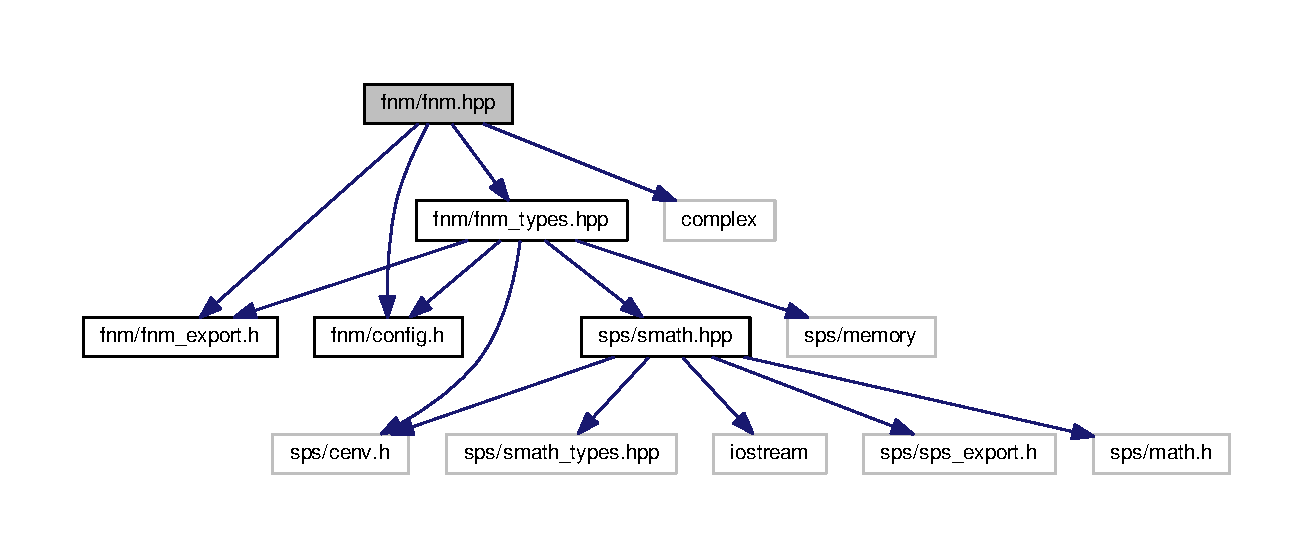
\includegraphics[width=350pt]{fnm_8hpp__incl}
\end{center}
\end{figure}
This graph shows which files directly or indirectly include this file\+:\nopagebreak
\begin{figure}[H]
\begin{center}
\leavevmode
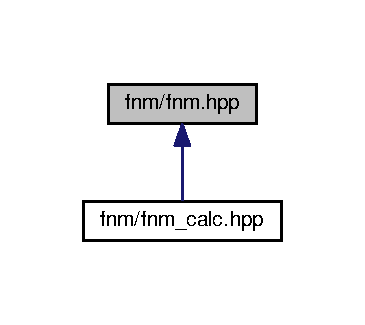
\includegraphics[width=175pt]{fnm_8hpp__dep__incl}
\end{center}
\end{figure}
\subsection*{Classes}
\begin{DoxyCompactItemize}
\item 
struct \hyperlink{singletonfnm_1_1ApertureData}{Aperture\+Data$<$ T $>$}
\begin{DoxyCompactList}\small\item\em Forward-\/declare \hyperlink{singletonfnm_1_1ApertureData}{Aperture\+Data}. \end{DoxyCompactList}\item 
class \hyperlink{classfnm_1_1Aperture}{Aperture$<$ T $>$}
\begin{DoxyCompactList}\small\item\em \hyperlink{classfnm_1_1Aperture}{Aperture} class. \end{DoxyCompactList}\end{DoxyCompactItemize}
\subsection*{Namespaces}
\begin{DoxyCompactItemize}
\item 
 \hyperlink{namespacefnm}{fnm}
\begin{DoxyCompactList}\small\item\em Fast Nearfield Method interfaces and implementations. \end{DoxyCompactList}\item 
 \hyperlink{namespacesps}{sps}
\end{DoxyCompactItemize}


\subsection{Detailed Description}
Contains Aperture class with methods using the fast nearfield method (F\+N\+M) 

\begin{DoxyAuthor}{Author}
Jens Munk Hansen \href{mailto:jens.munk.hansen@gmail.com}{\tt jens.\+munk.\+hansen@gmail.\+com} 
\end{DoxyAuthor}
\begin{DoxyDate}{Date}
Tue Jun 7 23\+:52\+:37 2016 
\end{DoxyDate}

\hypertarget{fnm__calc_8hpp}{\section{fnm/fnm\+\_\+calc.hpp File Reference}
\label{fnm__calc_8hpp}\index{fnm/fnm\+\_\+calc.\+hpp@{fnm/fnm\+\_\+calc.\+hpp}}
}


Function used for Fast-\/\+Nearfield-\/\+Method.  


{\ttfamily \#include $<$fnm/fnm.\+hpp$>$}\\*
{\ttfamily \#include $<$fnm\+\_\+data.\+hpp$>$}\\*
{\ttfamily \#include $<$sps/stdlib.\+h$>$}\\*
{\ttfamily \#include $<$complex$>$}\\*
Include dependency graph for fnm\+\_\+calc.\+hpp\+:\nopagebreak
\begin{figure}[H]
\begin{center}
\leavevmode
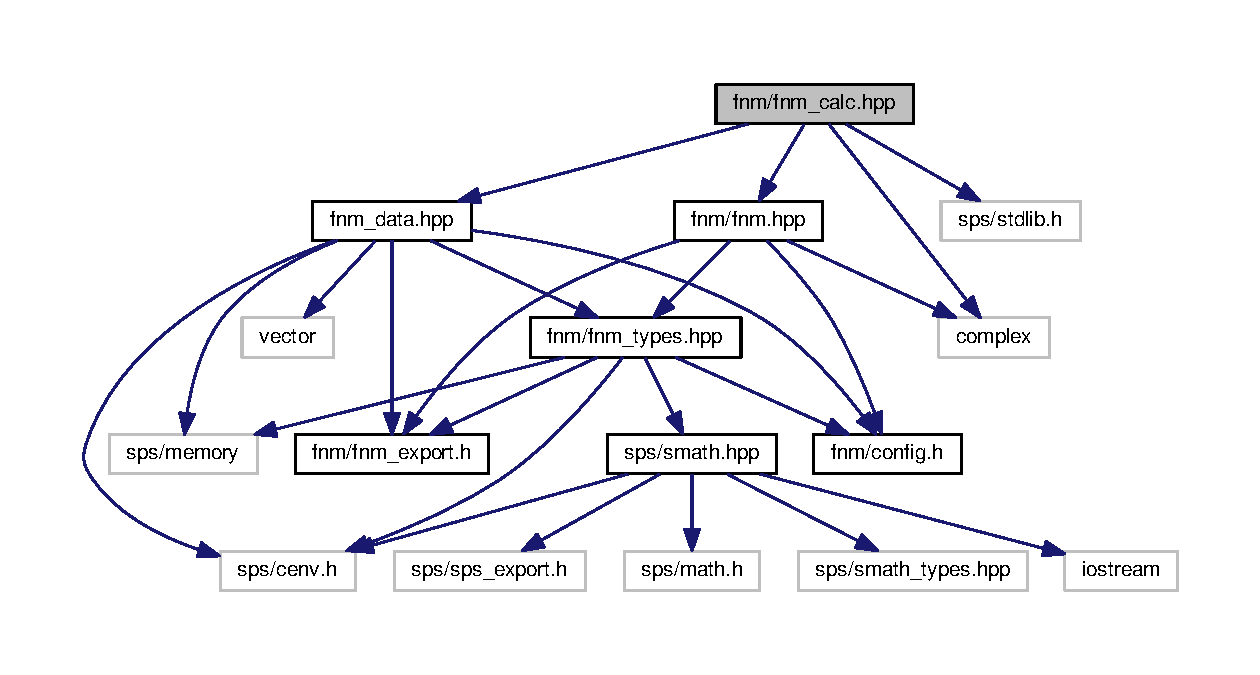
\includegraphics[width=350pt]{fnm__calc_8hpp__incl}
\end{center}
\end{figure}
\subsection*{Namespaces}
\begin{DoxyCompactItemize}
\item 
 \hyperlink{namespacefnm}{fnm}
\begin{DoxyCompactList}\small\item\em Fast Nearfield Method interfaces and implementations. \end{DoxyCompactList}\end{DoxyCompactItemize}
\subsection*{Functions}
\begin{DoxyCompactItemize}
\item 
{\footnotesize template$<$class T $>$ }\\std\+::complex$<$ T $>$ \hyperlink{namespacefnm_a1486ec1da93598ab2d37b17cf9f62252}{Calc\+Hz} (const T \&s, const T \&l, const T \&z, const T \&k, const T $\ast$uxs, const T $\ast$uweights, const size\+\_\+t n\+Us, const T $\ast$vxs, const T $\ast$vweights, const size\+\_\+t n\+Vs)
\item 
{\footnotesize template$<$class T $>$ }\\int \hyperlink{namespacefnm_a563d8aee788257300131ed9a7af75f64}{Calc\+Cw\+Field\+Ref} (const Aperture\+Data$<$ T $>$ \&data, const T $\ast$pos, const size\+\_\+t n\+Positions, std\+::complex$<$ T $>$ $\ast$$\ast$odata)
\item 
{\footnotesize template$<$class T $>$ }\\void \hyperlink{namespacefnm_a262768119606bb7e361e68564ba88829}{Calc\+Cw\+Field} (const Aperture\+Data$<$ T $>$ \&data, const T $\ast$pos, const size\+\_\+t n\+Positions, std\+::complex$<$ T $>$ $\ast$$\ast$odata)
\end{DoxyCompactItemize}


\subsection{Detailed Description}
Function used for Fast-\/\+Nearfield-\/\+Method. 

\begin{DoxyAuthor}{Author}
Jens Munk Hansen \href{mailto:jens.munk.hansen@gmail.com}{\tt jens.\+munk.\+hansen@gmail.\+com} 
\end{DoxyAuthor}
\begin{DoxyDate}{Date}
Mon Jun 13 08\+:33\+:33 2016 
\end{DoxyDate}

\hypertarget{fnm__data_8hpp}{\section{fnm/fnm\+\_\+data.hpp File Reference}
\label{fnm__data_8hpp}\index{fnm/fnm\+\_\+data.\+hpp@{fnm/fnm\+\_\+data.\+hpp}}
}
{\ttfamily \#include $<$fnm/fnm\+\_\+export.\+h$>$}\\*
{\ttfamily \#include $<$fnm/config.\+h$>$}\\*
{\ttfamily \#include $<$sps/cenv.\+h$>$}\\*
{\ttfamily \#include $<$sps/memory$>$}\\*
{\ttfamily \#include $<$fnm/fnm\+\_\+types.\+hpp$>$}\\*
{\ttfamily \#include $<$vector$>$}\\*
Include dependency graph for fnm\+\_\+data.\+hpp\+:\nopagebreak
\begin{figure}[H]
\begin{center}
\leavevmode
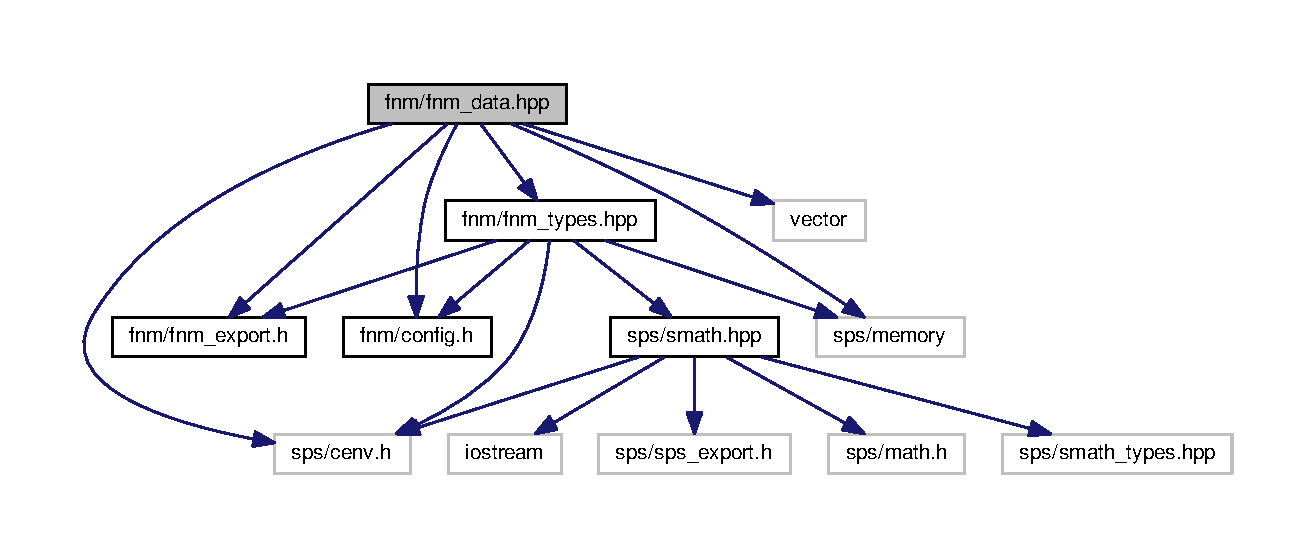
\includegraphics[width=350pt]{fnm__data_8hpp__incl}
\end{center}
\end{figure}
This graph shows which files directly or indirectly include this file\+:\nopagebreak
\begin{figure}[H]
\begin{center}
\leavevmode
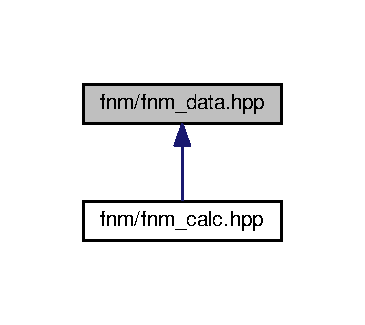
\includegraphics[width=175pt]{fnm__data_8hpp__dep__incl}
\end{center}
\end{figure}
\subsection*{Classes}
\begin{DoxyCompactItemize}
\item 
struct \hyperlink{singletonfnm_1_1ApertureData}{Aperture\+Data$<$ T $>$}
\begin{DoxyCompactList}\small\item\em Forward-\/declare \hyperlink{singletonfnm_1_1ApertureData}{Aperture\+Data}. \end{DoxyCompactList}\end{DoxyCompactItemize}
\subsection*{Namespaces}
\begin{DoxyCompactItemize}
\item 
 \hyperlink{namespacefnm}{fnm}
\begin{DoxyCompactList}\small\item\em Fast Nearfield Method interfaces and implementations. \end{DoxyCompactList}\end{DoxyCompactItemize}


\subsection{Detailed Description}
\begin{DoxyAuthor}{Author}
Jens Munk Hansen \href{mailto:jens.munk.hansen@gmail.com}{\tt jens.\+munk.\+hansen@gmail.\+com} 
\end{DoxyAuthor}
\begin{DoxyDate}{Date}
Thu Jun 9 06\+:12\+:31 2016 
\end{DoxyDate}

\hypertarget{fnm__types_8hpp}{\section{fnm/fnm\+\_\+types.hpp File Reference}
\label{fnm__types_8hpp}\index{fnm/fnm\+\_\+types.\+hpp@{fnm/fnm\+\_\+types.\+hpp}}
}
{\ttfamily \#include $<$fnm/config.\+h$>$}\\*
{\ttfamily \#include $<$fnm/fnm\+\_\+export.\+h$>$}\\*
{\ttfamily \#include $<$sps/cenv.\+h$>$}\\*
{\ttfamily \#include $<$sps/memory$>$}\\*
{\ttfamily \#include $<$sps/smath.\+hpp$>$}\\*
Include dependency graph for fnm\+\_\+types.\+hpp\+:\nopagebreak
\begin{figure}[H]
\begin{center}
\leavevmode
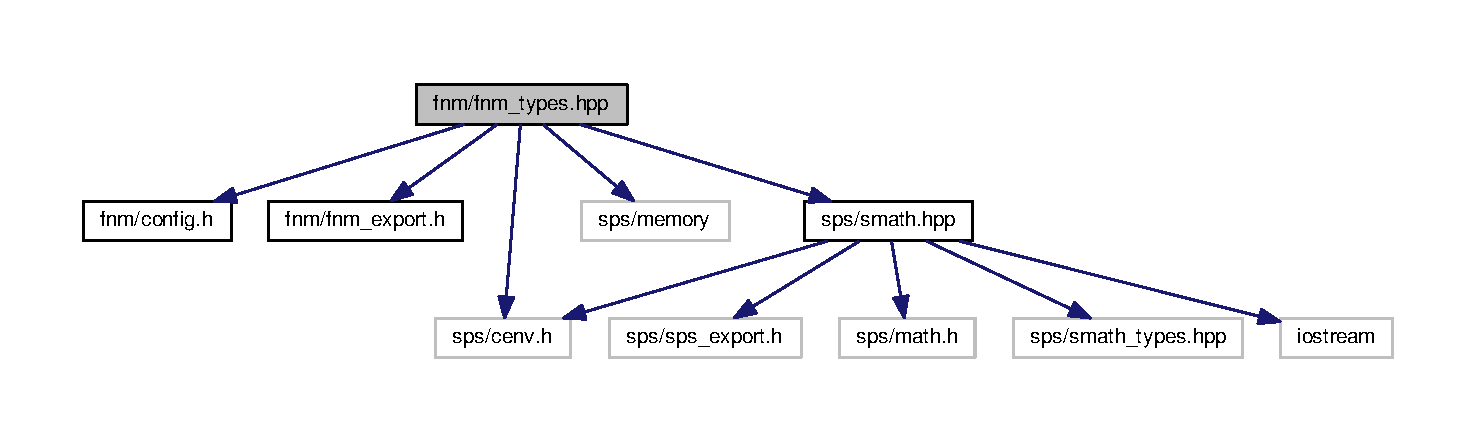
\includegraphics[width=350pt]{fnm__types_8hpp__incl}
\end{center}
\end{figure}
This graph shows which files directly or indirectly include this file\+:\nopagebreak
\begin{figure}[H]
\begin{center}
\leavevmode
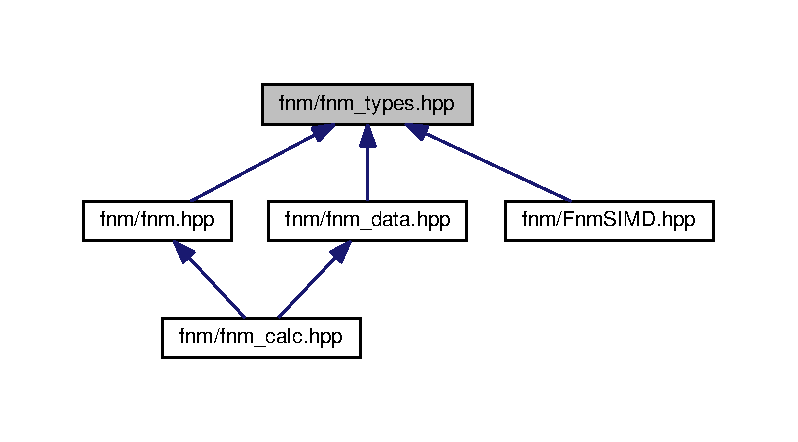
\includegraphics[width=350pt]{fnm__types_8hpp__dep__incl}
\end{center}
\end{figure}
\subsection*{Classes}
\begin{DoxyCompactItemize}
\item 
struct \hyperlink{structfnm_1_1sysparm__t}{sysparm\+\_\+t$<$ T $>$}
\begin{DoxyCompactList}\small\item\em Sysparm structure. \end{DoxyCompactList}\item 
struct \hyperlink{structfnm_1_1FocusingTypeNS}{Focusing\+Type\+N\+S}
\end{DoxyCompactItemize}
\subsection*{Namespaces}
\begin{DoxyCompactItemize}
\item 
 \hyperlink{namespacefnm}{fnm}
\begin{DoxyCompactList}\small\item\em Fast Nearfield Method interfaces and implementations. \end{DoxyCompactList}\end{DoxyCompactItemize}
\subsection*{Typedefs}
\begin{DoxyCompactItemize}
\item 
typedef Focusing\+Type\+N\+S\+::\+Value \hyperlink{namespacefnm_ac5c8ed1b3501db991ccb6065c89c3b54}{Focusing\+Type}
\end{DoxyCompactItemize}


\subsection{Detailed Description}
\begin{DoxyAuthor}{Author}
Jens Munk Hansen $<$jmh$>$ 
\end{DoxyAuthor}
\begin{DoxyDate}{Date}
Tue Oct 18 20\+:17\+:24 2016 
\end{DoxyDate}

\hypertarget{FnmMath_8hpp}{\section{fnm/\+Fnm\+Math.hpp File Reference}
\label{FnmMath_8hpp}\index{fnm/\+Fnm\+Math.\+hpp@{fnm/\+Fnm\+Math.\+hpp}}
}
{\ttfamily \#include $<$sps/smath.\+hpp$>$}\\*
{\ttfamily \#include $<$fnm/fnm\+\_\+export.\+h$>$}\\*
Include dependency graph for Fnm\+Math.\+hpp\+:\nopagebreak
\begin{figure}[H]
\begin{center}
\leavevmode
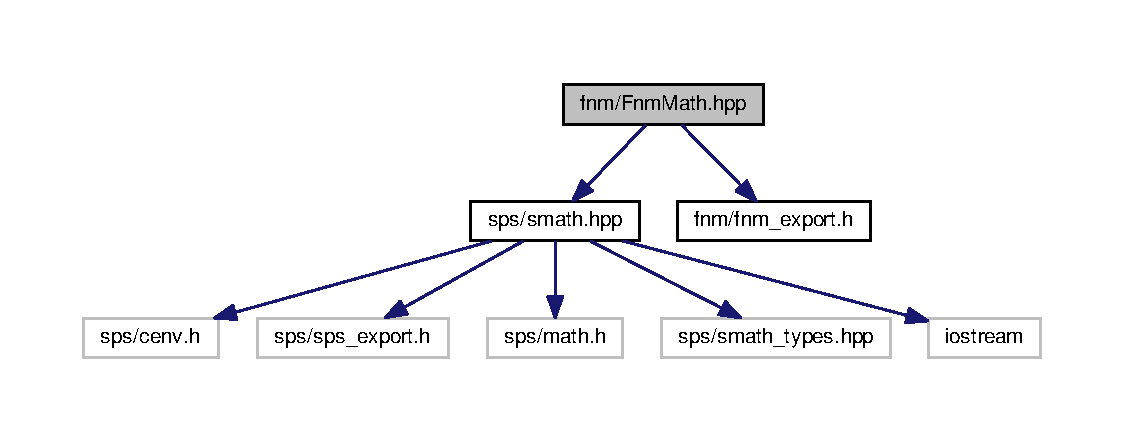
\includegraphics[width=350pt]{FnmMath_8hpp__incl}
\end{center}
\end{figure}
\subsection*{Classes}
\begin{DoxyCompactItemize}
\item 
struct \hyperlink{structfnm_1_1element__t}{element\+\_\+t$<$ T $>$}
\begin{DoxyCompactList}\small\item\em Element representation. \end{DoxyCompactList}\end{DoxyCompactItemize}
\subsection*{Namespaces}
\begin{DoxyCompactItemize}
\item 
 \hyperlink{namespacefnm}{fnm}
\begin{DoxyCompactList}\small\item\em Fast Nearfield Method interfaces and implementations. \end{DoxyCompactList}\end{DoxyCompactItemize}


\subsection{Detailed Description}
\begin{DoxyAuthor}{Author}
Jens Munk Hansen \href{mailto:jens.munk.hansen@gmail.com}{\tt jens.\+munk.\+hansen@gmail.\+com} 
\end{DoxyAuthor}
\begin{DoxyDate}{Date}
Thu Jun 9 06\+:00\+:01 2016 
\end{DoxyDate}

\hypertarget{FnmSIMD_8hpp}{\section{fnm/\+Fnm\+S\+I\+M\+D.hpp File Reference}
\label{FnmSIMD_8hpp}\index{fnm/\+Fnm\+S\+I\+M\+D.\+hpp@{fnm/\+Fnm\+S\+I\+M\+D.\+hpp}}
}
{\ttfamily \#include $<$fnm/config.\+h$>$}\\*
{\ttfamily \#include $<$sps/cenv.\+h$>$}\\*
{\ttfamily \#include $<$sps/smath.\+hpp$>$}\\*
{\ttfamily \#include $<$fnm/fnm\+\_\+types.\+hpp$>$}\\*
{\ttfamily \#include $<$sps/trigintrin.\+h$>$}\\*
{\ttfamily \#include $<$complex$>$}\\*
Include dependency graph for Fnm\+S\+I\+M\+D.\+hpp\+:\nopagebreak
\begin{figure}[H]
\begin{center}
\leavevmode
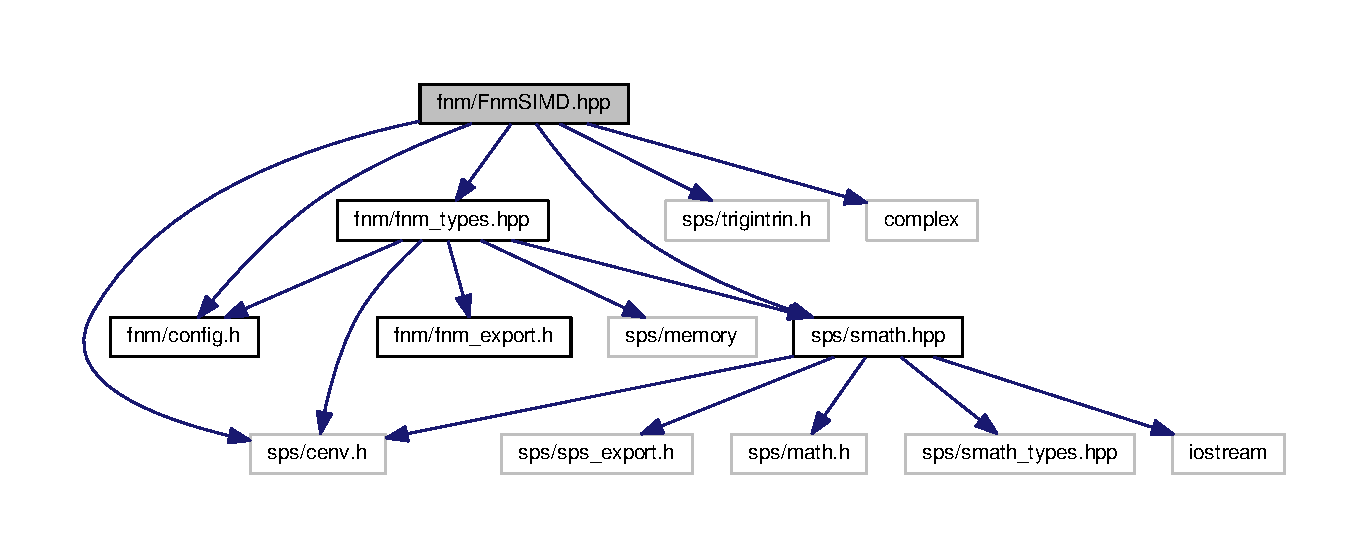
\includegraphics[width=350pt]{FnmSIMD_8hpp__incl}
\end{center}
\end{figure}
\subsection*{Functions}
\begin{DoxyCompactItemize}
\item 
{\footnotesize template$<$class T $>$ }\\S\+T\+A\+T\+I\+C\+\_\+\+I\+N\+L\+I\+N\+E\+\_\+\+B\+E\+G\+I\+N \\*
std\+::complex$<$ T $>$ \hyperlink{FnmSIMD_8hpp_aaf68820097524bc6a39eb9b5c95836e4}{Calc\+Hz\+Vec\+G\+L} (const T \&s, const T \&l, const T \&z, const T \&k, const T $\ast$us, const T $\ast$uweights, const size\+\_\+t n\+Us, const T $\ast$vs, const T $\ast$vweights, const size\+\_\+t n\+Vs) S\+T\+A\+T\+I\+C\+\_\+\+I\+N\+L\+I\+N\+E\+\_\+\+E\+N\+D
\item 
{\footnotesize template$<$class T $>$ }\\S\+T\+A\+T\+I\+C\+\_\+\+I\+N\+L\+I\+N\+E\+\_\+\+B\+E\+G\+I\+N \\*
std\+::complex$<$ T $>$ \hyperlink{FnmSIMD_8hpp_a15656136d30b6df89250c4d3ed1c3914}{Calc\+Hz\+All} (const sps\+::element\+\_\+t$<$ T $>$ \&element, const sps\+::point\+\_\+t$<$ T $>$ \&projection, const T \&k, const T $\ast$us, const T $\ast$uweights, const size\+\_\+t n\+Us, const T $\ast$vs, const T $\ast$vweights, const size\+\_\+t n\+Vs) S\+T\+A\+T\+I\+C\+\_\+\+I\+N\+L\+I\+N\+E\+\_\+\+E\+N\+D
\item 
{\footnotesize template$<$class T $>$ }\\S\+T\+A\+T\+I\+C\+\_\+\+I\+N\+L\+I\+N\+E\+\_\+\+B\+E\+G\+I\+N \\*
std\+::complex$<$ T $>$ \hyperlink{FnmSIMD_8hpp_a8c2f4b3432e306eb19be78d6e8636199}{Calc\+Hz\+Fast} (const sps\+::element\+\_\+t$<$ T $>$ \&element, const sps\+::point\+\_\+t$<$ T $>$ \&projection, const T \&k, const T $\ast$us, const T $\ast$uweights, const size\+\_\+t n\+Us, const T $\ast$vs, const T $\ast$vweights, const size\+\_\+t n\+Vs) S\+T\+A\+T\+I\+C\+\_\+\+I\+N\+L\+I\+N\+E\+\_\+\+E\+N\+D
\item 
{\footnotesize template$<$$>$ }\\std\+::complex$<$ float $>$ \hyperlink{FnmSIMD_8hpp_ada7ae13154936fbf393215429b6a8e67}{Calc\+Hz\+Vec\+G\+L} (const float \&s, const float \&l, const float \&z, const float \&k, const float $\ast$us, const float $\ast$uweights, const size\+\_\+t n\+Us, const float $\ast$vs, const float $\ast$vweights, const size\+\_\+t n\+Vs)
\item 
{\footnotesize template$<$$>$ }\\std\+::complex$<$ float $>$ \hyperlink{FnmSIMD_8hpp_a2afa33d436256506e69d6afd35552e58}{Calc\+Hz\+All} (const sps\+::element\+\_\+t$<$ float $>$ \&element, const sps\+::point\+\_\+t$<$ float $>$ \&projection, const float \&k, const float $\ast$us, const float $\ast$uweights, const size\+\_\+t n\+Us, const float $\ast$vs, const float $\ast$vweights, const size\+\_\+t n\+Vs)
\item 
{\footnotesize template$<$$>$ }\\std\+::complex$<$ float $>$ \hyperlink{FnmSIMD_8hpp_af714277fdda0c36cc35b950fc5178bc6}{Calc\+Hz\+Fast} (const sps\+::element\+\_\+t$<$ float $>$ \&element, const sps\+::point\+\_\+t$<$ float $>$ \&projection, const float \&k, const float $\ast$us, const float $\ast$uweights, const size\+\_\+t n\+Us, const float $\ast$vs, const float $\ast$vweights, const size\+\_\+t n\+Vs)
\item 
{\footnotesize template$<$$>$ }\\std\+::complex$<$ double $>$ \hyperlink{FnmSIMD_8hpp_ad78992ef7c633408569afdc5bf9c1959}{Calc\+Hz\+Fast} (const sps\+::element\+\_\+t$<$ double $>$ \&element, const sps\+::point\+\_\+t$<$ double $>$ \&projection, const double \&k, const double $\ast$us, const double $\ast$uweights, const size\+\_\+t n\+Us, const double $\ast$vs, const double $\ast$vweights, const size\+\_\+t n\+Vs)
\item 
{\footnotesize template$<$$>$ }\\std\+::complex$<$ double $>$ \hyperlink{FnmSIMD_8hpp_a483b42c4d0c798ba9bde31c0be682edd}{Calc\+Hz\+Vec\+G\+L} (const double \&s, const double \&l, const double \&z, const double \&k, const double $\ast$us, const double $\ast$uweights, const size\+\_\+t n\+Us, const double $\ast$vs, const double $\ast$vweights, const size\+\_\+t n\+Vs)
\item 
{\footnotesize template$<$$>$ }\\std\+::complex$<$ double $>$ \hyperlink{FnmSIMD_8hpp_a703837733eadf893395370bc38b77060}{Calc\+Hz\+All} (const sps\+::element\+\_\+t$<$ double $>$ \&element, const sps\+::point\+\_\+t$<$ double $>$ \&projection, const double \&k, const double $\ast$us, const double $\ast$uweights, const size\+\_\+t n\+Us, const double $\ast$vs, const double $\ast$vweights, const size\+\_\+t n\+Vs)
\end{DoxyCompactItemize}


\subsection{Detailed Description}
\begin{DoxyAuthor}{Author}
Jens Munk Hansen \href{mailto:jens.munk.hansen@gmail.com}{\tt jens.\+munk.\+hansen@gmail.\+com} 
\end{DoxyAuthor}
\begin{DoxyDate}{Date}
Thu Jun 9 06\+:01\+:12 2016 
\end{DoxyDate}


\subsection{Function Documentation}
\hypertarget{FnmSIMD_8hpp_a15656136d30b6df89250c4d3ed1c3914}{\index{Fnm\+S\+I\+M\+D.\+hpp@{Fnm\+S\+I\+M\+D.\+hpp}!Calc\+Hz\+All@{Calc\+Hz\+All}}
\index{Calc\+Hz\+All@{Calc\+Hz\+All}!Fnm\+S\+I\+M\+D.\+hpp@{Fnm\+S\+I\+M\+D.\+hpp}}
\subsubsection[{Calc\+Hz\+All}]{\setlength{\rightskip}{0pt plus 5cm}S\+T\+A\+T\+I\+C\+\_\+\+I\+N\+L\+I\+N\+E\+\_\+\+B\+E\+G\+I\+N std\+::complex$<$T$>$ Calc\+Hz\+All (
\begin{DoxyParamCaption}
\item[{const sps\+::element\+\_\+t$<$ T $>$ \&}]{element, }
\item[{const sps\+::point\+\_\+t$<$ T $>$ \&}]{projection, }
\item[{const T \&}]{k, }
\item[{const T $\ast$}]{us, }
\item[{const T $\ast$}]{uweights, }
\item[{const size\+\_\+t}]{n\+Us, }
\item[{const T $\ast$}]{vs, }
\item[{const T $\ast$}]{vweights, }
\item[{const size\+\_\+t}]{n\+Vs}
\end{DoxyParamCaption}
)}}\label{FnmSIMD_8hpp_a15656136d30b6df89250c4d3ed1c3914}
\hypertarget{FnmSIMD_8hpp_a2afa33d436256506e69d6afd35552e58}{\index{Fnm\+S\+I\+M\+D.\+hpp@{Fnm\+S\+I\+M\+D.\+hpp}!Calc\+Hz\+All@{Calc\+Hz\+All}}
\index{Calc\+Hz\+All@{Calc\+Hz\+All}!Fnm\+S\+I\+M\+D.\+hpp@{Fnm\+S\+I\+M\+D.\+hpp}}
\subsubsection[{Calc\+Hz\+All}]{\setlength{\rightskip}{0pt plus 5cm}std\+::complex$<$float$>$ Calc\+Hz\+All (
\begin{DoxyParamCaption}
\item[{const sps\+::element\+\_\+t$<$ float $>$ \&}]{element, }
\item[{const sps\+::point\+\_\+t$<$ float $>$ \&}]{projection, }
\item[{const float \&}]{k, }
\item[{const float $\ast$}]{us, }
\item[{const float $\ast$}]{uweights, }
\item[{const size\+\_\+t}]{n\+Us, }
\item[{const float $\ast$}]{vs, }
\item[{const float $\ast$}]{vweights, }
\item[{const size\+\_\+t}]{n\+Vs}
\end{DoxyParamCaption}
)\hspace{0.3cm}{\ttfamily [inline]}}}\label{FnmSIMD_8hpp_a2afa33d436256506e69d6afd35552e58}
\hypertarget{FnmSIMD_8hpp_a703837733eadf893395370bc38b77060}{\index{Fnm\+S\+I\+M\+D.\+hpp@{Fnm\+S\+I\+M\+D.\+hpp}!Calc\+Hz\+All@{Calc\+Hz\+All}}
\index{Calc\+Hz\+All@{Calc\+Hz\+All}!Fnm\+S\+I\+M\+D.\+hpp@{Fnm\+S\+I\+M\+D.\+hpp}}
\subsubsection[{Calc\+Hz\+All}]{\setlength{\rightskip}{0pt plus 5cm}std\+::complex$<$double$>$ Calc\+Hz\+All (
\begin{DoxyParamCaption}
\item[{const sps\+::element\+\_\+t$<$ double $>$ \&}]{element, }
\item[{const sps\+::point\+\_\+t$<$ double $>$ \&}]{projection, }
\item[{const double \&}]{k, }
\item[{const double $\ast$}]{us, }
\item[{const double $\ast$}]{uweights, }
\item[{const size\+\_\+t}]{n\+Us, }
\item[{const double $\ast$}]{vs, }
\item[{const double $\ast$}]{vweights, }
\item[{const size\+\_\+t}]{n\+Vs}
\end{DoxyParamCaption}
)\hspace{0.3cm}{\ttfamily [inline]}}}\label{FnmSIMD_8hpp_a703837733eadf893395370bc38b77060}
\hypertarget{FnmSIMD_8hpp_a8c2f4b3432e306eb19be78d6e8636199}{\index{Fnm\+S\+I\+M\+D.\+hpp@{Fnm\+S\+I\+M\+D.\+hpp}!Calc\+Hz\+Fast@{Calc\+Hz\+Fast}}
\index{Calc\+Hz\+Fast@{Calc\+Hz\+Fast}!Fnm\+S\+I\+M\+D.\+hpp@{Fnm\+S\+I\+M\+D.\+hpp}}
\subsubsection[{Calc\+Hz\+Fast}]{\setlength{\rightskip}{0pt plus 5cm}S\+T\+A\+T\+I\+C\+\_\+\+I\+N\+L\+I\+N\+E\+\_\+\+B\+E\+G\+I\+N std\+::complex$<$T$>$ Calc\+Hz\+Fast (
\begin{DoxyParamCaption}
\item[{const sps\+::element\+\_\+t$<$ T $>$ \&}]{element, }
\item[{const sps\+::point\+\_\+t$<$ T $>$ \&}]{projection, }
\item[{const T \&}]{k, }
\item[{const T $\ast$}]{us, }
\item[{const T $\ast$}]{uweights, }
\item[{const size\+\_\+t}]{n\+Us, }
\item[{const T $\ast$}]{vs, }
\item[{const T $\ast$}]{vweights, }
\item[{const size\+\_\+t}]{n\+Vs}
\end{DoxyParamCaption}
)}}\label{FnmSIMD_8hpp_a8c2f4b3432e306eb19be78d6e8636199}
Integral with (n\+Us x n\+Vs) points inside the region of integration


\begin{DoxyParams}{Parameters}
{\em element} & \\
\hline
{\em projection} & \\
\hline
{\em k} & \\
\hline
{\em us} & \\
\hline
{\em uweights} & \\
\hline
{\em n\+Us} & \\
\hline
{\em vs} & \\
\hline
{\em vweights} & \\
\hline
{\em n\+Vs} & \\
\hline
\end{DoxyParams}
\begin{DoxyReturn}{Returns}

\end{DoxyReturn}
\hypertarget{FnmSIMD_8hpp_af714277fdda0c36cc35b950fc5178bc6}{\index{Fnm\+S\+I\+M\+D.\+hpp@{Fnm\+S\+I\+M\+D.\+hpp}!Calc\+Hz\+Fast@{Calc\+Hz\+Fast}}
\index{Calc\+Hz\+Fast@{Calc\+Hz\+Fast}!Fnm\+S\+I\+M\+D.\+hpp@{Fnm\+S\+I\+M\+D.\+hpp}}
\subsubsection[{Calc\+Hz\+Fast}]{\setlength{\rightskip}{0pt plus 5cm}std\+::complex$<$float$>$ Calc\+Hz\+Fast (
\begin{DoxyParamCaption}
\item[{const sps\+::element\+\_\+t$<$ float $>$ \&}]{element, }
\item[{const sps\+::point\+\_\+t$<$ float $>$ \&}]{projection, }
\item[{const float \&}]{k, }
\item[{const float $\ast$}]{us, }
\item[{const float $\ast$}]{uweights, }
\item[{const size\+\_\+t}]{n\+Us, }
\item[{const float $\ast$}]{vs, }
\item[{const float $\ast$}]{vweights, }
\item[{const size\+\_\+t}]{n\+Vs}
\end{DoxyParamCaption}
)\hspace{0.3cm}{\ttfamily [inline]}}}\label{FnmSIMD_8hpp_af714277fdda0c36cc35b950fc5178bc6}
\hypertarget{FnmSIMD_8hpp_ad78992ef7c633408569afdc5bf9c1959}{\index{Fnm\+S\+I\+M\+D.\+hpp@{Fnm\+S\+I\+M\+D.\+hpp}!Calc\+Hz\+Fast@{Calc\+Hz\+Fast}}
\index{Calc\+Hz\+Fast@{Calc\+Hz\+Fast}!Fnm\+S\+I\+M\+D.\+hpp@{Fnm\+S\+I\+M\+D.\+hpp}}
\subsubsection[{Calc\+Hz\+Fast}]{\setlength{\rightskip}{0pt plus 5cm}std\+::complex$<$double$>$ Calc\+Hz\+Fast (
\begin{DoxyParamCaption}
\item[{const sps\+::element\+\_\+t$<$ double $>$ \&}]{element, }
\item[{const sps\+::point\+\_\+t$<$ double $>$ \&}]{projection, }
\item[{const double \&}]{k, }
\item[{const double $\ast$}]{us, }
\item[{const double $\ast$}]{uweights, }
\item[{const size\+\_\+t}]{n\+Us, }
\item[{const double $\ast$}]{vs, }
\item[{const double $\ast$}]{vweights, }
\item[{const size\+\_\+t}]{n\+Vs}
\end{DoxyParamCaption}
)\hspace{0.3cm}{\ttfamily [inline]}}}\label{FnmSIMD_8hpp_ad78992ef7c633408569afdc5bf9c1959}
\hypertarget{FnmSIMD_8hpp_aaf68820097524bc6a39eb9b5c95836e4}{\index{Fnm\+S\+I\+M\+D.\+hpp@{Fnm\+S\+I\+M\+D.\+hpp}!Calc\+Hz\+Vec\+G\+L@{Calc\+Hz\+Vec\+G\+L}}
\index{Calc\+Hz\+Vec\+G\+L@{Calc\+Hz\+Vec\+G\+L}!Fnm\+S\+I\+M\+D.\+hpp@{Fnm\+S\+I\+M\+D.\+hpp}}
\subsubsection[{Calc\+Hz\+Vec\+G\+L}]{\setlength{\rightskip}{0pt plus 5cm}S\+T\+A\+T\+I\+C\+\_\+\+I\+N\+L\+I\+N\+E\+\_\+\+B\+E\+G\+I\+N std\+::complex$<$T$>$ Calc\+Hz\+Vec\+G\+L (
\begin{DoxyParamCaption}
\item[{const T \&}]{s, }
\item[{const T \&}]{l, }
\item[{const T \&}]{z, }
\item[{const T \&}]{k, }
\item[{const T $\ast$}]{us, }
\item[{const T $\ast$}]{uweights, }
\item[{const size\+\_\+t}]{n\+Us, }
\item[{const T $\ast$}]{vs, }
\item[{const T $\ast$}]{vweights, }
\item[{const size\+\_\+t}]{n\+Vs}
\end{DoxyParamCaption}
)}}\label{FnmSIMD_8hpp_aaf68820097524bc6a39eb9b5c95836e4}
\hypertarget{FnmSIMD_8hpp_ada7ae13154936fbf393215429b6a8e67}{\index{Fnm\+S\+I\+M\+D.\+hpp@{Fnm\+S\+I\+M\+D.\+hpp}!Calc\+Hz\+Vec\+G\+L@{Calc\+Hz\+Vec\+G\+L}}
\index{Calc\+Hz\+Vec\+G\+L@{Calc\+Hz\+Vec\+G\+L}!Fnm\+S\+I\+M\+D.\+hpp@{Fnm\+S\+I\+M\+D.\+hpp}}
\subsubsection[{Calc\+Hz\+Vec\+G\+L}]{\setlength{\rightskip}{0pt plus 5cm}std\+::complex$<$float$>$ Calc\+Hz\+Vec\+G\+L (
\begin{DoxyParamCaption}
\item[{const float \&}]{s, }
\item[{const float \&}]{l, }
\item[{const float \&}]{z, }
\item[{const float \&}]{k, }
\item[{const float $\ast$}]{us, }
\item[{const float $\ast$}]{uweights, }
\item[{const size\+\_\+t}]{n\+Us, }
\item[{const float $\ast$}]{vs, }
\item[{const float $\ast$}]{vweights, }
\item[{const size\+\_\+t}]{n\+Vs}
\end{DoxyParamCaption}
)\hspace{0.3cm}{\ttfamily [inline]}}}\label{FnmSIMD_8hpp_ada7ae13154936fbf393215429b6a8e67}
\hypertarget{FnmSIMD_8hpp_a483b42c4d0c798ba9bde31c0be682edd}{\index{Fnm\+S\+I\+M\+D.\+hpp@{Fnm\+S\+I\+M\+D.\+hpp}!Calc\+Hz\+Vec\+G\+L@{Calc\+Hz\+Vec\+G\+L}}
\index{Calc\+Hz\+Vec\+G\+L@{Calc\+Hz\+Vec\+G\+L}!Fnm\+S\+I\+M\+D.\+hpp@{Fnm\+S\+I\+M\+D.\+hpp}}
\subsubsection[{Calc\+Hz\+Vec\+G\+L}]{\setlength{\rightskip}{0pt plus 5cm}std\+::complex$<$double$>$ Calc\+Hz\+Vec\+G\+L (
\begin{DoxyParamCaption}
\item[{const double \&}]{s, }
\item[{const double \&}]{l, }
\item[{const double \&}]{z, }
\item[{const double \&}]{k, }
\item[{const double $\ast$}]{us, }
\item[{const double $\ast$}]{uweights, }
\item[{const size\+\_\+t}]{n\+Us, }
\item[{const double $\ast$}]{vs, }
\item[{const double $\ast$}]{vweights, }
\item[{const size\+\_\+t}]{n\+Vs}
\end{DoxyParamCaption}
)\hspace{0.3cm}{\ttfamily [inline]}}}\label{FnmSIMD_8hpp_a483b42c4d0c798ba9bde31c0be682edd}

\hypertarget{swig__system_8h}{\section{fnm/swig\+\_\+system.h File Reference}
\label{swig__system_8h}\index{fnm/swig\+\_\+system.\+h@{fnm/swig\+\_\+system.\+h}}
}

\hypertarget{bessel__lut_8hpp}{\section{gl/bessel\+\_\+lut.hpp File Reference}
\label{bessel__lut_8hpp}\index{gl/bessel\+\_\+lut.\+hpp@{gl/bessel\+\_\+lut.\+hpp}}
}


Look up tables L\+U\+Ts for Bessel functions.  


{\ttfamily \#include $<$gl/config.\+h$>$}\\*
{\ttfamily \#include $<$gl/gl\+\_\+export.\+h$>$}\\*
Include dependency graph for bessel\+\_\+lut.\+hpp\+:\nopagebreak
\begin{figure}[H]
\begin{center}
\leavevmode
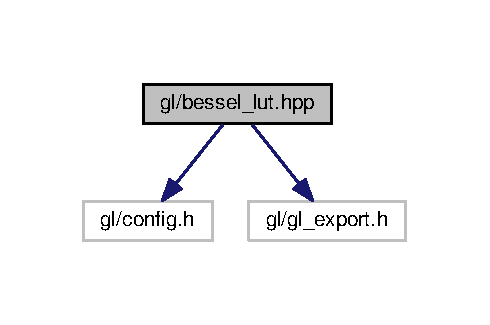
\includegraphics[width=235pt]{bessel__lut_8hpp__incl}
\end{center}
\end{figure}
\subsection*{Namespaces}
\begin{DoxyCompactItemize}
\item 
 \hyperlink{namespacegl}{gl}
\begin{DoxyCompactList}\small\item\em Gauss-\/\+Legendre interfaces and implementations. \end{DoxyCompactList}\end{DoxyCompactItemize}
\subsection*{Variables}
\begin{DoxyCompactItemize}
\item 
double \hyperlink{namespacegl_af3f8ce6ef90f2939af71d4dcd7f7300b}{J\+Z} \mbox{[}\+\_\+\+B\+E\+S\+S\+E\+L\+J\+Z\+E\+R\+O\+\_\+\+L\+U\+T\+\_\+\+T\+A\+B\+L\+E\+\_\+\+S\+I\+Z\+E\mbox{]}
\item 
double \hyperlink{namespacegl_a3f45d860f72d97fe1d1fb1e5fa4749ff}{J1} \mbox{[}\+\_\+\+B\+E\+S\+S\+E\+L\+J\+\_\+1\+\_\+\+S\+Q\+U\+A\+R\+E\+D\+\_\+\+L\+U\+T\+\_\+\+T\+A\+B\+L\+E\+\_\+\+S\+I\+Z\+E\mbox{]}
\end{DoxyCompactItemize}


\subsection{Detailed Description}
Look up tables L\+U\+Ts for Bessel functions. 

\begin{DoxyAuthor}{Author}
Jens Munk Hansen \href{mailto:jens.munk.hansen@gmail.com}{\tt jens.\+munk.\+hansen@gmail.\+com} 
\end{DoxyAuthor}
\begin{DoxyDate}{Date}
Tue Jun 21 21\+:11\+:51 2016 
\end{DoxyDate}

\hypertarget{gl_8hpp}{\section{gl/gl.hpp File Reference}
\label{gl_8hpp}\index{gl/gl.\+hpp@{gl/gl.\+hpp}}
}


Gauss-\/\+Legendre integration library.  


{\ttfamily \#include $<$gl/gl\+\_\+export.\+h$>$}\\*
{\ttfamily \#include $<$gl/config.\+h$>$}\\*
{\ttfamily \#include $<$stddef.\+h$>$}\\*
Include dependency graph for gl.\+hpp\+:\nopagebreak
\begin{figure}[H]
\begin{center}
\leavevmode
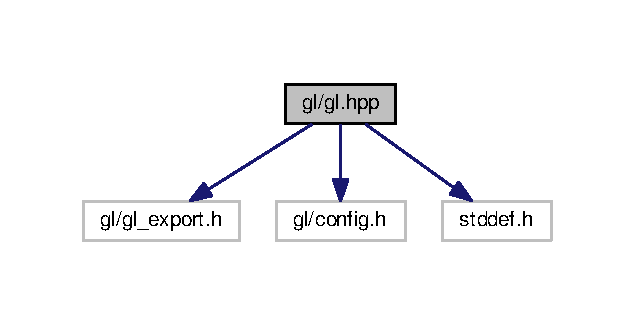
\includegraphics[width=305pt]{gl_8hpp__incl}
\end{center}
\end{figure}
\subsection*{Classes}
\begin{DoxyCompactItemize}
\item 
struct \hyperlink{structgl_1_1GLNode}{G\+L\+Node}
\begin{DoxyCompactList}\small\item\em Container for weight and nodes. \end{DoxyCompactList}\end{DoxyCompactItemize}
\subsection*{Namespaces}
\begin{DoxyCompactItemize}
\item 
 \hyperlink{namespacegl}{gl}
\begin{DoxyCompactList}\small\item\em Gauss-\/\+Legendre interfaces and implementations. \end{DoxyCompactList}\end{DoxyCompactItemize}
\subsection*{Functions}
\begin{DoxyCompactItemize}
\item 
double G\+L\+\_\+\+E\+X\+P\+O\+R\+T \hyperlink{namespacegl_a8dfc38fe28db34846c60086d6ecf508c}{G\+L\+Quad} (size\+\_\+t n, double($\ast$f)(double, void $\ast$), void $\ast$data, double a, double b)
\item 
\hyperlink{structgl_1_1GLNode}{gl\+::\+G\+L\+Node} G\+L\+\_\+\+E\+X\+P\+O\+R\+T \hyperlink{namespacegl_aa2fa29b0a69c2eeb23b4e0b9613e7fc5}{G\+L} (size\+\_\+t l, size\+\_\+t k)
\item 
\hyperlink{structgl_1_1GLNode}{gl\+::\+G\+L\+Node} G\+L\+\_\+\+E\+X\+P\+O\+R\+T \hyperlink{namespacegl_a7f251958ee6d2c65e37b0f9e61a9fe30}{G\+L\+S} (size\+\_\+t n, size\+\_\+t k)
\item 
double G\+L\+\_\+\+E\+X\+P\+O\+R\+T \hyperlink{namespacegl_a516dc08710fc7a9d7f455203bcd9a358}{besseljzero} (int k)
\item 
double G\+L\+\_\+\+E\+X\+P\+O\+R\+T \hyperlink{namespacegl_a8a87a797409c579a3658648f68de3d8a}{besselj1squared} (int k)
\end{DoxyCompactItemize}


\subsection{Detailed Description}
Gauss-\/\+Legendre integration library. 

\begin{DoxyAuthor}{Author}
Jens Munk Hansen \href{mailto:jens.munk.hansen@gmail.com}{\tt jens.\+munk.\+hansen@gmail.\+com} 
\end{DoxyAuthor}
\begin{DoxyDate}{Date}
Mon Jun 20 21\+:11\+:40 2016 
\end{DoxyDate}

\hypertarget{gl__lut_8hpp}{\section{gl/gl\+\_\+lut.hpp File Reference}
\label{gl__lut_8hpp}\index{gl/gl\+\_\+lut.\+hpp@{gl/gl\+\_\+lut.\+hpp}}
}


Look up tables L\+U\+Ts with weight and values for Gauss-\/\+Legendre knots.  


{\ttfamily \#include $<$gl/config.\+h$>$}\\*
{\ttfamily \#include $<$gl/gl\+\_\+export.\+h$>$}\\*
Include dependency graph for gl\+\_\+lut.\+hpp\+:\nopagebreak
\begin{figure}[H]
\begin{center}
\leavevmode
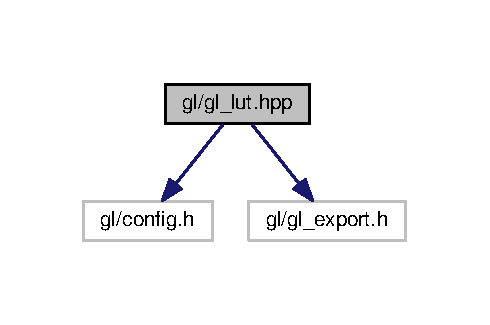
\includegraphics[width=235pt]{gl__lut_8hpp__incl}
\end{center}
\end{figure}
\subsection*{Namespaces}
\begin{DoxyCompactItemize}
\item 
 \hyperlink{namespacegl}{gl}
\begin{DoxyCompactList}\small\item\em Gauss-\/\+Legendre interfaces and implementations. \end{DoxyCompactList}\end{DoxyCompactItemize}
\subsection*{Variables}
\begin{DoxyCompactItemize}
\item 
const double $\ast$ \hyperlink{namespacegl_af4c9c0a0468b7e8a4a075d536afd6f65}{weights} \mbox{[}\+\_\+\+G\+L\+\_\+\+L\+U\+T\+\_\+\+T\+A\+B\+L\+E\+\_\+\+S\+I\+Z\+E\mbox{]}
\item 
const double $\ast$ \hyperlink{namespacegl_a8fd2242d1215dfb011d971d994f6aea5}{abcissas} \mbox{[}\+\_\+\+G\+L\+\_\+\+L\+U\+T\+\_\+\+T\+A\+B\+L\+E\+\_\+\+S\+I\+Z\+E\mbox{]}
\end{DoxyCompactItemize}


\subsection{Detailed Description}
Look up tables L\+U\+Ts with weight and values for Gauss-\/\+Legendre knots. 

\begin{DoxyAuthor}{Author}
Jens Munk Hansen \href{mailto:jens.munk.hansen@gmail.com}{\tt jens.\+munk.\+hansen@gmail.\+com} 
\end{DoxyAuthor}
\begin{DoxyDate}{Date}
Wed Jun 22 13\+:22\+:00 2016 
\end{DoxyDate}

\hypertarget{smath_8hpp}{\section{sps/smath.hpp File Reference}
\label{smath_8hpp}\index{sps/smath.\+hpp@{sps/smath.\+hpp}}
}


Simple math.  


{\ttfamily \#include $<$sps/cenv.\+h$>$}\\*
{\ttfamily \#include $<$sps/sps\+\_\+export.\+h$>$}\\*
{\ttfamily \#include $<$sps/math.\+h$>$}\\*
{\ttfamily \#include $<$sps/smath\+\_\+types.\+hpp$>$}\\*
{\ttfamily \#include $<$iostream$>$}\\*
Include dependency graph for smath.\+hpp\+:\nopagebreak
\begin{figure}[H]
\begin{center}
\leavevmode
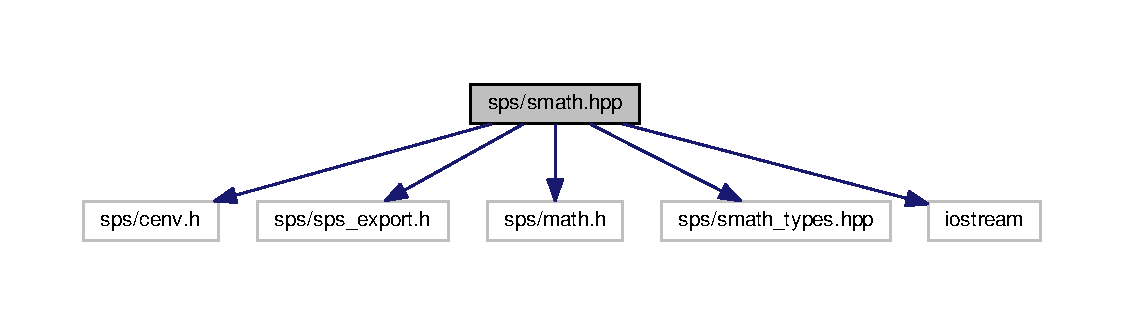
\includegraphics[width=350pt]{smath_8hpp__incl}
\end{center}
\end{figure}
This graph shows which files directly or indirectly include this file\+:\nopagebreak
\begin{figure}[H]
\begin{center}
\leavevmode
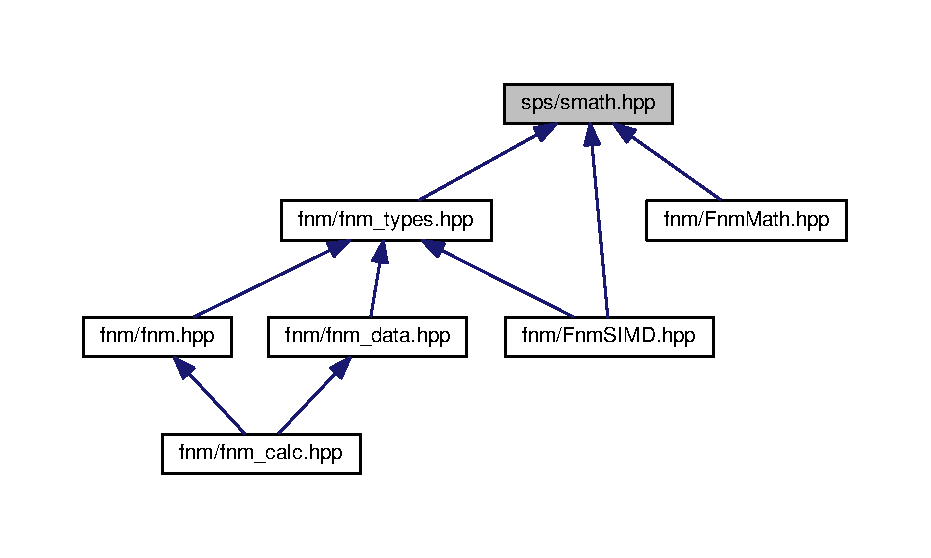
\includegraphics[width=350pt]{smath_8hpp__dep__incl}
\end{center}
\end{figure}
\subsection*{Namespaces}
\begin{DoxyCompactItemize}
\item 
 \hyperlink{namespacesps}{sps}
\end{DoxyCompactItemize}
\subsection*{Functions}
\begin{DoxyCompactItemize}
\item 
{\footnotesize template$<$typename T $>$ }\\constexpr int \hyperlink{smath_8hpp_ab50269cb12c04295c021f7ce24108750}{signum} (T x, std\+::false\+\_\+type is\+\_\+signed)
\item 
{\footnotesize template$<$typename T $>$ }\\constexpr int \hyperlink{smath_8hpp_a6ad435c3cf741e6cf8d6c2ed5c272210}{signum} (T x, std\+::true\+\_\+type is\+\_\+signed)
\item 
{\footnotesize template$<$typename T $>$ }\\constexpr int \hyperlink{smath_8hpp_a4761435ab54306df78fcba4fd156e3fd}{signum} (T x)
\item 
{\footnotesize template$<$class T $>$ }\\T \hyperlink{namespacesps_a5ec8f80252d9d984138f014c822d27d0}{dist\+\_\+point\+\_\+to\+\_\+point} (const point\+\_\+t$<$ T $>$ \&a, const point\+\_\+t$<$ T $>$ \&b)
\item 
{\footnotesize template$<$typename T $>$ }\\T \hyperlink{namespacesps_a49b7bc999932466978a16485e1c6a98b}{dot} (const point\+\_\+t$<$ T $>$ \&a, const point\+\_\+t$<$ T $>$ \&b)
\item 
{\footnotesize template$<$typename T $>$ }\\point\+\_\+t$<$ T $>$ \hyperlink{namespacesps_a634cb0a93cc6f57c45c79f7df04c8752}{operator-\/} (const point\+\_\+t$<$ T $>$ \&a, const point\+\_\+t$<$ T $>$ \&b)
\item 
{\footnotesize template$<$typename T $>$ }\\point\+\_\+t$<$ T $>$ \hyperlink{namespacesps_abcd3fabeb60a10d9ad05fc027c789e9e}{operator+} (const point\+\_\+t$<$ T $>$ \&a, const point\+\_\+t$<$ T $>$ \&b)
\item 
{\footnotesize template$<$typename T $>$ }\\point\+\_\+t$<$ T $>$ \hyperlink{namespacesps_a04c7b1f1585fda60325b43c35937ee96}{cross} (const point\+\_\+t$<$ T $>$ \&a, const point\+\_\+t$<$ T $>$ \&b)
\item 
{\footnotesize template$<$typename T $>$ }\\point\+\_\+t$<$ T $>$ \hyperlink{namespacesps_a22175b6c56edce28e060aaddb0443215}{operator$\ast$} (const T \&a, const point\+\_\+t$<$ T $>$ \&b)
\item 
{\footnotesize template$<$typename T $>$ }\\T \hyperlink{namespacesps_ac8e58e03b1ed250e4dd83774401fb670}{norm} (const point\+\_\+t$<$ T $>$ \&a)
\item 
{\footnotesize template$<$typename T $>$ }\\T \hyperlink{namespacesps_a55c6fe1c1fdf3c5a3e7b354dae205840}{dist\+\_\+to\+\_\+line} (const point\+\_\+t$<$ T $>$ \&point, const point\+\_\+t$<$ T $>$ \&point\+On\+Line, const point\+\_\+t$<$ T $>$ \&direction)
\item 
{\footnotesize template$<$typename T $>$ }\\T \hyperlink{namespacesps_a6d00662f3287276d877ae3e1e10b9c6e}{sgn\+\_\+dist\+\_\+to\+\_\+plane} (const point\+\_\+t$<$ T $>$ \&point, const point\+\_\+t$<$ T $>$ \&point\+On\+Plane, const point\+\_\+t$<$ T $>$ \&unit\+Normal)
\item 
{\footnotesize template$<$typename T $>$ }\\sps\+::point\+\_\+t$<$ T $>$ \hyperlink{namespacesps_a4cbe6332a0c07b3bb2e80bb8048d6f9e}{clamp\+\_\+vector} (const sps\+::point\+\_\+t$<$ T $>$ \&point, const sps\+::bbox\+\_\+t$<$ T $>$ \&box)
\item 
{\footnotesize template$<$typename T $>$ }\\sps\+::point\+\_\+t$<$ T $>$ \hyperlink{namespacesps_a49f2545f74f9a6cf30e04d428badaf27}{nearest\+\_\+point\+\_\+on\+\_\+bbox} (const sps\+::point\+\_\+t$<$ T $>$ \&point, const sps\+::bbox\+\_\+t$<$ T $>$ \&box)
\item 
{\footnotesize template$<$typename T $>$ }\\sps\+::point\+\_\+t$<$ T $>$ \hyperlink{namespacesps_a5ba962916e1ba5c3114e45f153d80081}{farthest\+\_\+point\+\_\+on\+\_\+bbox} (const sps\+::point\+\_\+t$<$ T $>$ \&point, const sps\+::bbox\+\_\+t$<$ T $>$ \&box)
\item 
{\footnotesize template$<$typename T $>$ }\\void \hyperlink{namespacesps_a00bcbe34e177c2a5ac0ec59f89998db2}{dists\+\_\+most\+\_\+distant\+\_\+and\+\_\+closest} (const sps\+::bbox\+\_\+t$<$ T $>$ \&box0, const sps\+::bbox\+\_\+t$<$ T $>$ \&box1, T $\ast$dist\+Near, T $\ast$dist\+Far)
\item 
{\footnotesize template$<$typename T $>$ }\\void S\+P\+S\+\_\+\+E\+X\+P\+O\+R\+T \hyperlink{namespacesps_af6fa4d5ae05cae25226c8f79d864a722}{basis\+\_\+vectors} (sps\+::point\+\_\+t$<$ T $>$ \&output, const sps\+::euler\+\_\+t$<$ T $>$ \&euler, size\+\_\+t index)
\item 
{\footnotesize template$<$typename T $>$ }\\void S\+P\+S\+\_\+\+E\+X\+P\+O\+R\+T \hyperlink{namespacesps_a1f2f198c4ef4cd43756c6d07dfcbd790}{basis\+\_\+vectors} (T $\ast$vec0, T $\ast$vec1, T $\ast$vec2, const sps\+::euler\+\_\+t$<$ T $>$ \&euler)
\item 
{\footnotesize template$<$typename T $>$ }\\std\+::ostream \& \hyperlink{namespacesps_a1f6bfb41fd1c17ffbe559cb6c9838487}{operator$<$$<$} (std\+::ostream \&out, const point\+\_\+t$<$ T $>$ \&point)
\end{DoxyCompactItemize}


\subsection{Detailed Description}
Simple math. 

\begin{DoxyAuthor}{Author}
Jens Munk Hansen \href{mailto:jens.munk.hansen@gmail.com}{\tt jens.\+munk.\+hansen@gmail.\+com} 
\end{DoxyAuthor}
\begin{DoxyDate}{Date}
Sat Oct 10 18\+:41\+:43 2015 
\end{DoxyDate}


\subsection{Function Documentation}
\hypertarget{smath_8hpp_ab50269cb12c04295c021f7ce24108750}{\index{smath.\+hpp@{smath.\+hpp}!signum@{signum}}
\index{signum@{signum}!smath.\+hpp@{smath.\+hpp}}
\subsubsection[{signum}]{\setlength{\rightskip}{0pt plus 5cm}constexpr int signum (
\begin{DoxyParamCaption}
\item[{T}]{x, }
\item[{std\+::false\+\_\+type}]{is\+\_\+signed}
\end{DoxyParamCaption}
)\hspace{0.3cm}{\ttfamily [inline]}}}\label{smath_8hpp_ab50269cb12c04295c021f7ce24108750}
Signum function


\begin{DoxyParams}{Parameters}
{\em x} & \\
\hline
{\em is\+\_\+signed} & \\
\hline
\end{DoxyParams}
\begin{DoxyReturn}{Returns}

\end{DoxyReturn}
\hypertarget{smath_8hpp_a6ad435c3cf741e6cf8d6c2ed5c272210}{\index{smath.\+hpp@{smath.\+hpp}!signum@{signum}}
\index{signum@{signum}!smath.\+hpp@{smath.\+hpp}}
\subsubsection[{signum}]{\setlength{\rightskip}{0pt plus 5cm}constexpr int signum (
\begin{DoxyParamCaption}
\item[{T}]{x, }
\item[{std\+::true\+\_\+type}]{is\+\_\+signed}
\end{DoxyParamCaption}
)\hspace{0.3cm}{\ttfamily [inline]}}}\label{smath_8hpp_a6ad435c3cf741e6cf8d6c2ed5c272210}
Signum function


\begin{DoxyParams}{Parameters}
{\em x} & \\
\hline
{\em is\+\_\+signed} & \\
\hline
\end{DoxyParams}
\begin{DoxyReturn}{Returns}

\end{DoxyReturn}
\hypertarget{smath_8hpp_a4761435ab54306df78fcba4fd156e3fd}{\index{smath.\+hpp@{smath.\+hpp}!signum@{signum}}
\index{signum@{signum}!smath.\+hpp@{smath.\+hpp}}
\subsubsection[{signum}]{\setlength{\rightskip}{0pt plus 5cm}constexpr int signum (
\begin{DoxyParamCaption}
\item[{T}]{x}
\end{DoxyParamCaption}
)\hspace{0.3cm}{\ttfamily [inline]}}}\label{smath_8hpp_a4761435ab54306df78fcba4fd156e3fd}
Signum function


\begin{DoxyParams}{Parameters}
{\em x} & \\
\hline
\end{DoxyParams}
\begin{DoxyReturn}{Returns}

\end{DoxyReturn}


Here is the call graph for this function\+:\nopagebreak
\begin{figure}[H]
\begin{center}
\leavevmode
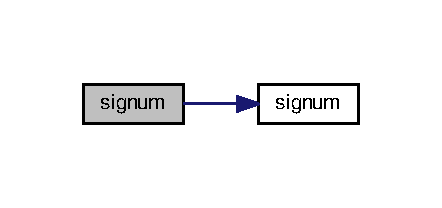
\includegraphics[width=212pt]{smath_8hpp_a4761435ab54306df78fcba4fd156e3fd_cgraph}
\end{center}
\end{figure}



%--- End generated contents ---

% Index
\newpage
\phantomsection
\addcontentsline{toc}{chapter}{Index}
\printindex

\end{document}
